% !TEX root = ../main.tex

\chapter{Patanalysis}
\label{ch:analysis}

\startcontents[chapters]

\vfill

\begin{alltt}\sffamily
Where thou mayst knock a nail into his head,
but near him thy angel becomes a fear,
it must omit real necessities,
hear Faith infringed which such zeal did swear.

With sighs in an odd angle of the isle,
before me to sweet beds of flow,
might quench the zeal of all professors else,
the whilst his iron did on the anvil cool.

Intend a kind of zeal both to the Prince and Claudio,
and threescore year would make the world away,
nay if you read this line.

Have no delight to pass away the time,
by a shadow like an angel,
four nights will quickly dream away the time.
\end{alltt}

\newpage
\begin{figure}[!htbp]
\centering
  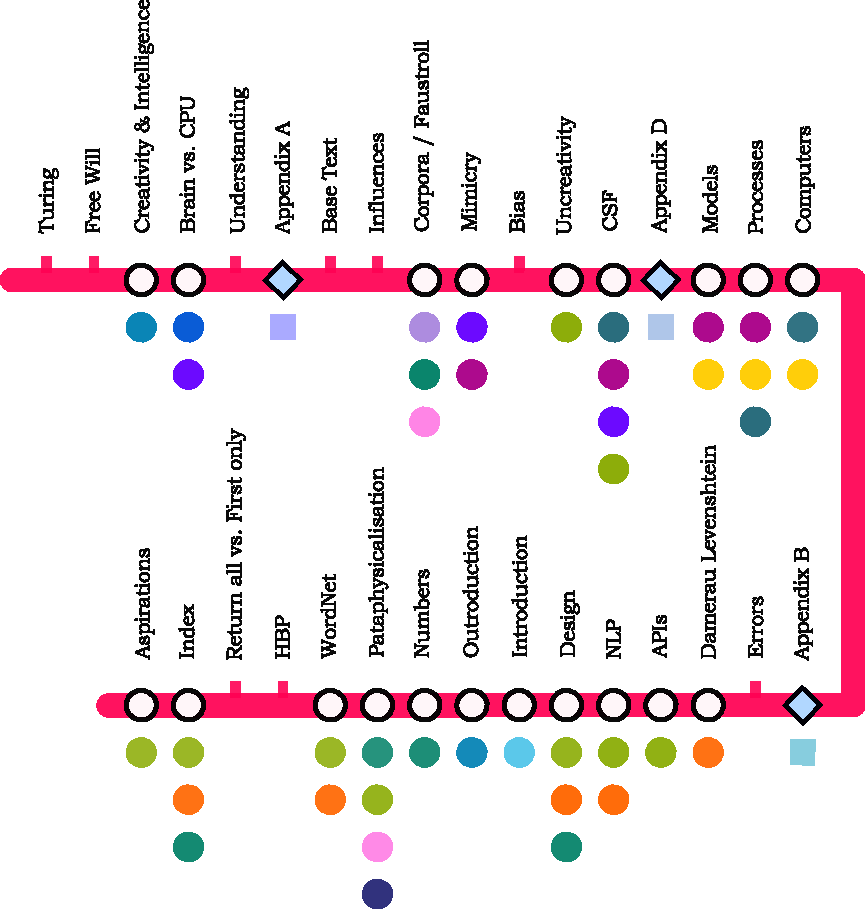
\includegraphics{anal.pdf}
\end{figure}

\vfill

{\sffamily 
Hello World \intro, test vlah blah dhfsdhf sdifh sohdsld hf sdfh h ghdls hg. Hello World \intro, whats up \inspi~ and helllo to you too \appa~ test,. ksjdfkj sdkjgh  ksdhg sdjfh sdjfh ksdfjhsdkfhskh kgh kjhfdg kjhgfhjfh sjueyuh tyb jjhg.
Hello World \intro, test vlah blah dhfsdhf sdifh sohdsld hf sdfh h ghdls hg. Hello World \intro, whats up \inspi~ and helllo to you too \appa~ test,. ksjdfkj sdkjgh  ksdhg sdjfh sdjfh ksdfjhsdkfhskh kgh kjhfdg kjhgfhjfh sjueyuh tyb jjhg.
Hello World \intro, test vlah blah dhfsdhf sdifh sohdsld hf sdfh h ghdls hg. Hello World \intro, whats up \inspi~ and helllo to you too \appa~ test,. ksjdfkj sdkjgh  ksdhg sdjfh sdjfh ksdfjhsdkfhskh kgh kjhfdg kjhgfhjfh sjueyuh tyb jjhg.
}

\begin{figure}[!htbp]
\centering
  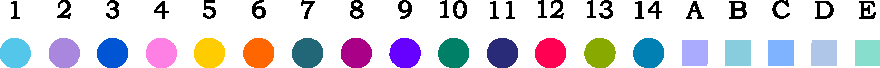
\includegraphics[width=\textwidth]{legend.pdf}
\end{figure}

\newpage
\minicontents
\spirals

A lot of the more theoretical aspects of this research have been discussed in the \nameref{ch:foundations}\marginpar{§~\ref{ch:foundations}~\&~\ref{ch:interpretation}} and \nameref{ch:interpretation} chapters. The evaluation here is more concerned with the practical artefact \url{pata.physics.wtf} and its interpretation.

This chapter is divided into several sections addressing issues related to \url{pata.physics.wtf}. This includes a discussion of the inspirations, an analysis of some of the technical aspects, a review of design decisions made, a contextualisation and also a meta-analysis of the project's execution and management.


\section{Influences}

Looking back over the inspirations for this project described in chapter~\ref{ch:inspirations}\marginpar{§~\ref{ch:inspirations}}, some of the influences can be clearly seen straight away. Others are intentionally a bit more subtle. There are various motivations for that. First, transparency conflicts with surprise. \emph{Serendipity} was one of the original aims to try and model, so being overly obvious and descriptive about what the tool is and does would be counter productive. An element of surprise also makes it more enjoyable in repeat visits. Pure randomness is meaningless. Another reason was \emph{humour}. Pataphysics has an intrinsic kind of humour I wanted to include in the whole presentation of the artefact. 

\begin{description}
  \item[Syzygy Surfer]\marginpar{§~\ref{s:surfer}} The influence of the \textit{Syzygy Surfer} cannot be overstated. It forms the immediate predecessor to my research. The authors of the \textit{Syzygy Surfer} are part of my supervisory team. This is where the initial ideas for the pataphysical algorithms\marginpar{§~\ref{s:algorithms}} came from. There are important differences as well though. For example, pataphors were never implemented as originally suggested. The idea of using ontologies and semantic web technologies such as \ac{RDF} to develop the system was abandoned early on too.
  \item[Faustroll Library]\marginpar{§~\ref{s:faustlib}} This fictional library of real books was direct inspiration for the Faustroll corpus used in the text search\marginpar{§~\ref{s:corpora}}. I tried my best to complete the library as accurately as I could but some of the texts where unsourceable. As with the original, I included some foreign language texts. Since the results (if the Faustroll corpus is chosen of course) are drawn from any of these texts, the mood and style of language is quite distinct and atmospheric.
  \item[Queneau's $\bm{10^{14}}$ poems]\marginpar{§~\ref{s:queneau}} Queneau is another one of the inspirations that became a direct influence. The text search can be displayed as poetry\marginpar{§~\ref{s:poetry}} in the same style as Queneau's 100 thousand million poems, only in digital form and with a larger set of lines. This means that many more possible poems can be generated by switching individual lines.
  \item[Chinese Encyclopedia]\marginpar{§~\ref{s:borges}} Borges' story has been an inspiration right from the start. The subtle humour in it is great. The sort of semantic logic behind it was modeled through the pataphysical algorithms\marginpar{§~\ref{s:algorithms}}.
  \item[Yossarian]\marginpar{§~\ref{s:yossarian}} The metaphorical algorithms are intriguing but elusive---I wasn't able to find any details on their implementation. This may be due to the nature of the project, which is commercial rather than academic. It is hard to compare against this site as it is so different even though we share some of the same goals or principles.
  \item[Library of Babel]\marginpar{§~\ref{s:babel}} The library of babel is a great project which has only indirectly influenced my work. The pataphysical elements in it are obvious even though perhaps unconscious. The seriousness with which the library is presented, the pseudo-scientific approach, the vagueness of what's actually behind it. Is it random? Or is it indeed the most gigantic digital library of any book every written or ever to be written? The sheer perceived scale of the library was part motivation for calculating the numbers of the generatable poems\marginpar{\faicon{table}~\ref{tab:faustshake}}.
  \item[Oulipo]\marginpar{§~\ref{s:oulipo}} Given that the \ac{OULIPO} is directly rooted in pataphysical principles\footnote{Remember that the \ac{OULIPO} was founded as a subcommittee of the ``Coll\`{e}ge de 'Pataphysique'' in the 60's.}, the influence on this project cannot be overstated. The algorithms\marginpar{§~\ref{s:algorithms}} created could even be seen as an Oulipian technique themselves.
  \item[Coder Culture]\marginpar{§~\ref{s:culture}} This group of inspirations is a bit more generic and influenced lots of little things throughout the project. The idea of hiding easter eggs on the site, the deliberate placement or use of errors, the obfuscation, the humour, the jargonisation and littered `l33t' style language, and the art and aesthetics behind it. All of that---and most of all perhaps: this thesis---was influenced by coder culture.
\end{description}


\section{Pataphysicalisation}
\label{s:pataphyanalysis}

As mentioned in chapter~\ref{s:pataputers}\marginpar{§~\ref{s:pataputers}}, the internal transformation of a query term to the final results is what I called the \emph{pataphysicalisation} process. The three pataphysical algorithms (Clinamen, Syzygy and Antinomy), or \emph{patalgorithms}, are at the center of this process. 

\begin{enumerate}
  \item User enters single query term,
  \item system transforms query term into list of pataphysicalised terms (patadata),
  \item system retrieves sentence fragments containing keywords from this list,
  \item system displays sentence fragments in various formats.
\end{enumerate}

It is quite interesting to compare the algorithms with each other. By removing the clutter (in this case the sentence surrounding the pataphysicalised keyword) we can see a few example results side by side in table~\ref{tab:algorithmscomp}.

\begin{table}[!htbp]
\caption[Comparison of patalgorithms]{Comparison of patalgorithms showing a selection of results for each}
\label{tab:algorithmscomp}
  \begin{tabu}{X[1,L]X[3,L]X[3,L]X[2,L]}
  \toprule
  % \cline{2-4}
  \textbf{Query} & \textbf{Clinamen} & \textbf{Syzygy} & \textbf{Antinomy}
  \\ \midrule
  \textbf{clear}
  &
  altar, leaf, pleas, cellar
  &
  vanish, allow, bare, pronounce
  &
  opaque
  \\ \cmidrule{1-4}
  \textbf{solid}
  &
  sound, valid, solar, slide
  &
  block, form, matter, crystal, powder
  &
  liquid, hollow
  \\ \cmidrule{1-4}
  \textbf{books}
  &
  boot, bones, hooks, rocks, banks
  &
  dialogue, authority, record, fact
  &
  ---
  \\ \cmidrule{1-4}
  \textbf{troll}
  &
  grill, role, tell
  &
  wheel, roll, mouth, speak
  &
  ---
  \\ \cmidrule{1-4}
  \textbf{live}
  &
  love, lies, river, wave, size, bite
  &
  breathe, people, domicile, taste, see, be
  &
  recorded, dead
  \\ \bottomrule
  \end{tabu}
\end{table}

Seeing the results in a table like\marginpar{\faicon{table}~\ref{tab:algorithmscomp}} this gives an almost immediate idea of how each algorithm works. This is not meant to be transparent and perhaps only after knowing the ins and outs of the algorithms can one recognise how each result was found. 

The clinamen results show words that contain one or two spelling errors of the original query term. It is perhaps counter-intuitive to have words such as `altar', `leaf' and `cellar' be classed as spelling errors of the word `clear' but they clearly could be. Remember that a spelling error can be classed in one of four ways: (1) deletion, (2) insertion, (3) substitution and (4) transposition. So, going from `clear' to `altar' is an instance of two times case 3 (`c' is replace by `a' and `e' is replaced by `t') and going from  `clear' to `leaf' is an example of case 1 (`c' is deleted) and case 3 (`r' is replaced by `f').

Looking at the second column (the syzygy results) shows the semantic relationship between the original query term and the results. Again, this may not be immediately noticeable but certainly once you know how the process works you can recognise the common relations. This is especially evident for the antinomy algorithm which is based on opposites.

\spirals

However it is equally interesting to compare some full sentences. Looking at some of the poems at the beginning of each chapter shows the variety of the possible outcomes (see pages \pageref{ch:introduction}, \pageref{ch:inspirations}, \pageref{ch:methodology}, \pageref{ch:pataphysics}, \pageref{ch:creativity}, \pageref{ch:technology}, \pageref{ch:evaluation}, \pageref{ch:foundations}, \pageref{ch:interpretation}, \pageref{ch:implementation}, \pageref{ch:applications}, \pageref{ch:analysis}, \pageref{ch:future}, and \pageref{ch:observations}). It also highlights the difference between the two corpora. Poems based on the Faustroll corpus have a very different sound and feel to it than ones based on the Shakespeare corpus.

\begin{figure}[!htbp]
\centering
\begin{minipage}{.45\linewidth}
  \settowidth{\versewidth}{earth was flat like the floor of an Oven}
  % \PoemTitle{Flower}
  \begin{verse}[\versewidth]\sffamily\footnotesize
    There was a period put to the Fire\\
    pink and spot\\
    earth was flat like the floor of an Oven\\
    as much ease as a mower doth the grass

    during the first period of my captivity\\
    room with a hard earthen floor\\
    not within everyone's power\\
    or your favourite flowers died

    shocks lose power\\
    the white daisy\\
    after a long period

    poppy\\
    peony\\
    stock to all People
  \end{verse}
\end{minipage}
\hspace{.02\linewidth}
\begin{minipage}{.45\linewidth}
  \settowidth{\versewidth}{led by their master to the flow'red fields}
  % \PoemTitle{Flower}
  \begin{verse}[\versewidth]\sffamily\footnotesize
    O bloody period\\
    I as your lover speak\\
    has she such power\\
    gather those flowers

    thy lover\\
    juiced flowers\\
    had I been any god of power\\
    or a lover's lute

    the river hath thrice flow'd\\
    but sad mortality o'ersways their power\\
    now here a period of tumultuous broils

    led by their master to the flow'red fields\\
    not a minister in his power\\
    where soulds do couch on flowers
  \end{verse}
\end{minipage}
\caption[Faustroll vs. Shakespeare poetry]{Comparison of Faustroll (left) versus Shakespeare (right) poetry, both for query term `flower'}
\label{fig:2poems}
\end{figure}

Sometimes we can even get a general feel for the theme of the poem, as in we can recognize the connection, the relationship between the individual lines and what must be the original query term. Of course putting the poems into the chapters as they are---without specifically stating the keyword they were generated from or the corpus they are based on---makes them a bit more elusive.

The different language is quite obvious. This is helped by the fact that the Shakespeare corpus is of course written by the same author\footnote{Unless we believe the legends that Shakespeare didn't write those works by himself\ldots}. The Faustroll corpus contains text by over 20 different authors and in three different languages even.


\subsection{Numbers}
\label{s:numbers}

The above examples (table~\ref{tab:algorithmscomp} and figure~\ref{fig:2poems}) give a good overview of the two main factors in the pataphysicalisation process, namely the three patalgorithms and the two corpora. Both only reflect a small selection of the variety of results produced though. It is therefore quite interesting to look at some actual numbers.

\begin{table}[!htbp]
\caption[Faustroll vs. Shakespeare in numbers]{Faustroll versus Shakespeare in numbers}
\label{tab:faustshake}
  \centering
  \begin{tabu}{llcccc}
  \toprule
  \textbf{Query} & \textbf{Corpus} & \textbf{Results} & \textbf{Reverbs} & \textbf{Origins} & \textbf{Poems}\\
  \midrule
  \multirow{2}{*}{flower} & Faustroll   & \num{90}   & \num{25} & \num{18} & \num{7.8e10}\\
                          & Shakespeare & \num{158}  & \num{15} & \num{38} & \num{3.8e14}\\
  \cmidrule{1-6}
  \multirow{2}{*}{clear}  & Faustroll   & \num{542}  & \num{79} & \num{23} & \num{1.3e22}\\
                          & Shakespeare & \num{1445} & \num{72} & \num{38} & \num{1.5e28}\\
  \cmidrule{1-6}
  \multirow{2}{*}{troll}  & Faustroll   & \num{124}  & \num{16} & \num{16} & \num{4.4e12}\\
                          & Shakespeare & \num{327}  & \num{14} & \num{38} & \num{1.1e19}\\
  \cmidrule{1-6}
  \multirow{2}{*}{fania}  & Faustroll   & \num{9}    & \num{2}  & \num{6}  & \num{1}\\
                          & Shakespeare & \num{15}   & \num{2}  & \num{14} & \num{1}\\
  \bottomrule
  \end{tabu}
\end{table}

Table~\ref{tab:faustshake}\marginpar{\faicon{table}~\ref{tab:faustshake}} shows a comparison of the two different corpora with four example query terms.

\begin{description}
  \item[Results] A `result' in this case is one line (a sentence fragment). This column shows the total number of results found by the three algorithms combined. Individual results appear only once but the keyword it contains can appear in several of the results.
  \item[Reverbs] A `reverberation' is one of the terms in the list of keywords (patadata) produced by the pataphysicalisation process. The list cannot contain duplicates but each reverberation can appear in more than one result. Reverberations are used to find results in each corpus. This column shows the total number of reverberations created by the three algorithms.
  \item[Origins] An `origin' in this case is the original source text from which a given sentence fragment was retrieved. Each corpus has a set number of source texts. Each origin can contain several results based on several reverberations. This column shows the number of origins in the given corpus in which results were found.
  \item[Poems] This refers to the total number of Queneau style poems that can be generated using the given results\footnote{The original book by Queneau contains 10 sonnets with 14 lines each. This means the total number of possible poems generated by different combinations of lines in the book is $10^{14}$ or one hundred thousand million.}. This is calculated as the number of different options per line to the power of the number of lines.
\end{description}

To put this into perspective, the Faustroll corpus contains a total of \num{28} texts of very varied authors and different languages even. This might explain why the queries in table~\ref{tab:faustshake}\marginpar{\faicon{table}~\ref{tab:faustshake}} have not found results in all of the texts. The query `clear' found results in \num{23} out of \num{28} for example while the query `fania' only found results in \num{6} texts. The Shakespeare corpus seems much more uniform. Reverberations generally seem to find results in all \num{38} source texts in the corpus apart from the query `fania'. This might be explained by the fact that Shakespeare wrote all of the texts himself using much of the same language and vocabulary unlike the Faustroll corpus. 

It is rather interesting to note that even though the Shakespeare corpus produces overall more results from more texts, the Faustroll corpus produces more reverberations per query. This might stem from the multi-author, multi-language nature of the corpus. The overall vocabulary\marginpar{§~\ref{s:index}} used is much larger than the Shakespeare one (see subsections \nameref{s:fauststats} and \nameref{s:shakestats} at the end of this chapter).

Regarding the final column showing the number of possible poems, let's look at the `Shakespeare---clear' row. There are 1445 results. These are spread over 14 lines, so each line has 103 options. The overall number of poems is therefore calculated as $103^{14}$ which equals \num{15125897248551112432256145169} (or \num{1.5e28} in short\marginpar{\faicon{table}~\ref{tab:faustshake}}).

\spirals

A slightly different angle to consider is a comparison of these kind of numbers between each of the algorithms. Table~\ref{tab:algonums}\marginpar{\faicon{table}~\ref{tab:algonums}} shows the numbers of results, reverberations and origins for the Clinamen, Syzygy and Antinomy algorithms using five example query terms (`clear', `shine', `disorder', `stuck', and `feather') for each of the two corpora (`Faustroll' and `Shakespeare').

\begin{table}[!htbp]
\caption[Numbers per algorithm]{Results-Reverberations-Origin numbers per algorithm}
\label{tab:algonums}
\centering\small
\begin{tabu}{ll|ccc|ccc|ccc|ccc}
\toprule
 & & \multicolumn{3}{c}{\textbf{Clinamen}} & \multicolumn{3}{c}{\textbf{Syzygy}} & \multicolumn{3}{c|}{\textbf{Antinomy}} & \multicolumn{3}{c}{} \\ 
\cmidrule{3-11}
\multicolumn{1}{l}{} & \textbf{Query} & \rotatebox{90}{Results} & \rotatebox{90}{Reverbs} & \rotatebox{90}{Origins} & \rotatebox{90}{Results} & \rotatebox{90}{Reverbs} & \rotatebox{90}{Origins} & \rotatebox{90}{Results} & \rotatebox{90}{Reverbs} & \rotatebox{90}{Origins} & \multicolumn{3}{c}{\textbf{Total}} \\ 
\midrule
\multicolumn{1}{l}{\multirow{4}{*}{\textbf{\rotatebox{90}{Faustroll}}}} 
& clear & 158 & 20 & 13 & 368 & 90 & 23 & 16 & 8 & 8 & \multicolumn{3}{c}{542--79--23} \\
\multicolumn{1}{l}{} 
& shine & 228 & 29 & 19 & 154 & 61 & 16 & 0 & 0 & 0 & \multicolumn{3}{c}{382--61--20} \\
\multicolumn{1}{l}{}
& disorder & 0 & 0 & 0 & 159 & 127 & 23 & 10 & 2 & 10 & \multicolumn{3}{c}{169--40--23} \\
\multicolumn{1}{l}{}
& stuck & 59 & 14 & 13 & 181 & 43 & 22 & 11 & 3 & 9 & \multicolumn{3}{c}{251--47--22} \\ 
\multicolumn{1}{l}{}
& feather & 78 & 13 & 12 & 83 & 37 & 14 & 0 & 0 & 0 & \multicolumn{3}{c}{161--29--14} \\[0.5cm] 
\cmidrule{1-12}
\multicolumn{1}{l}{\multirow{4}{*}{\textbf{\rotatebox{90}{Shakespeare}}}}
& clear & 435 & 20 & 38 & 997 & 90 & 38 & 13 & 8 & 12 & \multicolumn{3}{c}{1445--72--38} \\
\multicolumn{1}{l}{}
& shine & 575 & 29 & 38 & 333 & 61 & 38 & 0 & 0 & 0 & \multicolumn{3}{c}{908--53--38} \\
\multicolumn{1}{l}{}
& disorder & 0 & 0 & 0 & 326 & 127 & 38 & 29 & 2 & 29 & \multicolumn{3}{c}{355--26--38} \\
\multicolumn{1}{l}{}
& stuck & 152 & 14 & 37 & 479 & 43 & 38 & 34 & 3 & 34 & \multicolumn{3}{c}{665--41--38} \\ 
\multicolumn{1}{l}{}
& feather & 217 & 13 & 38 & 195 & 37 & 38 & 0 & 0 & 0 & \multicolumn{3}{c}{412--25--38} \\ 
\bottomrule
\end{tabu}
\end{table}

The first immediate observation surely must be that the Antinomy algorithm produces the fewest results, in four cases even none at all. This is caused by the fact that the Antinomy algorithm\marginpar{§~\ref{s:antinomyalgo}} is based on semantic opposites in WordNet and some words simply do not have defined opposites. Addressing this issue was left for future work mentioned in chapter~\ref{ch:future}\marginpar{§~\ref{ch:future}}. On the other hand the Syzygy algorithm\marginpar{§~\ref{s:syzygyalgo}}, which is also based on WordNet, produces most results on average.

The Clinamen algorithm\marginpar{§~\ref{s:clinamenalgo}} interestingly produces a varying number of results depending on the query term. For the query `disorder' no results were found in either the Faustroll or the Shakespeare corpus. This of course is rooted in the fact that no reverberations were produced during the pataphysicalisation process. Here it is important to remember that the Clinamen algorithm makes use of a base document\footnote{This is hardcoded to be Jarry's \textit{Exploits and Opinions of Doctor Faustroll, Pataphysician}. Section~\ref{s:basetext} discusses what would happen if we changed the base document to something else.}\marginpar{§~\ref{s:basetext}}. Therefore the success of the algorithm depends on the vocabulary of this base text. In this particular example this means that there was no word in the base text of one or two spelling errors to the original query of `disorder'.

Looking at the origins column in table~\ref{tab:algonums}\marginpar{\faicon{table}~\ref{tab:algonums}} highlights how the Shakespeare corpus mostly produces results from each of its 38 texts. The Faustroll corpus varies a lot more. This may be due to the different languages and varying word counts of the files in the corpus.

\subsubsection{Faustroll}
\label{s:fauststats}
\begin{itemize}
  \item There are three empty texts (Peladan, de Chilra, de Regnier).
  \item The total number of words is \num{1738461}. Of this, \num{1204158} words are from English texts (70\%), \num{497144} are French (28\%) and \num{37159} are in German (2\%).
  \item The shortest text contains \num{3853} words (Coleridge).
  \item The longest text contains \num{419456} words (Poe).
  \item The average amount of words per text is \num{62088}.
  \item The vocabulary of the index contains \num{78893} words. Of this \num{49040} are English terms.
\end{itemize}

\subsubsection{Shakespeare}
\label{s:shakestats}
\begin{itemize}
  \item The total number of words is \num{883460}\footnote{According to \autocite{Efron1976} Shakespeare used \num{31534} different words in his works, about half of which he only used once (\num{14376}). They cite the total number of words used in his corpus as \num{884647}.}.
  \item The shortest text contains \num{2568} words (Lover's Complaint).
  \item The longest text contains \num{32031} words (Hamlet).
  \item The average amount of words per text is \num{23249}.
  \item The vocabulary of the index contains \num{23398} words.
\end{itemize}

It should be noted that the index\marginpar{§~\ref{s:index}} is generated based on the texts vocabulary minus stopwords. Stopwords (e.g. `and', `or', `the', etc.) are common terms that occur frequently in use. The full list of stopwords per language can be found in appendix~\ref{s:stopwords}\marginpar{§~\ref{s:stopwords}}.


\subsection{Sentences}
\label{s:sents}

The index stores entries in the following format (for more detail see chapter~\ref{s:index}\marginpar{§~\ref{s:index}}).

\begin{minted}{text}
{
  word1: {fileA: [pos1, pos2, ...], fileB: [pos1], ...},
  word2: {fileC: [pos1, pos2], fileK: [pos1, pos2, pos3, ...], ...},
  ...
}
\end{minted}

At the top level we have a list of words. Each word contains a list of files and each file stores a list of positions. After the pataphysicalisation process, any entries in the index that match the pataphysicalised query terms are looked up and then the corresponding sentences are retrieved to display as results. The code is set up to retrieve the first position only instead of each one, referred to as the \emph{first only} method from now on (see source~\ref{code:ppsent}\marginpar{\faicon{code}~\ref{code:ppsent}}).

\begin{minted}{text}
{
  word1: {fileA: [pos1], fileB: [pos1], ...},
  word2: {fileC: [pos1], fileK: [pos1], ...},
  ...
}
\end{minted}

This has two implications: (1) there is some unnecessary computation at the startup of the program when the index is generated and (2) only a fraction of the possible results are retrieved.

The decision to only use one position was mainly made for performance issues. Generating the full results with each position (the \emph{return all} method) takes a lot more time than doing it for just the first occurance. This is perhaps best understood by looking at an example.

The Faustroll corpus produces \num{542} results for the query `clear' with only the first sentence. If we enable the retrieval of every matching sentence, the number of results increases to \num{8751}.

\begin{minted}{text}
cellar: {l_19: [4448, 18718, 68678, 110318, 192486, 267241, 352502, 352565]}
\end{minted}

The above pseudocode shows an entry for the word `cellar' with only the positions for the \py{l_19} file\footnote{Fran\c{c}ois Rabelais: Gargantua and Pantagruel}. Another example of an index entry for the term `doctor' can be found on page~\pageref{c:pos}. The sentences for the above positions are shown below. Using only the first occurance (position) means the system ignores the rest.

\begin{description}[leftmargin=2.2cm]
  \item[4448] ``rope wine is let down into a cellar''
  \item[18718] ``bread and holy water of the cellar''
  \item[68678] ``year who had a cool cellar under ground''
  \item[110318] ``cellar''
  \item[192486] ``that Nick in the dark cellar''
  \item[267241] ``on the cellar door''
  \item[352502] ``in mind of the painted cellar in the oldest city in the world''
  \item[352565] ``and the painted cellar also''
\end{description}

Table~\ref{tab:percent}\marginpar{\faicon{table}~\ref{tab:percent}} shows some example queries for both corpora and the number of results retrieved with the first position only used (as in the live version of \url{pata.physics.wtf}) in column 5 and on column 3 with all results retrieved. The final column shows what percentage of results are retrieved using the `first only' method. The average percentage for this is about 10\%. 

\begin{table}[!htbp]
\caption[Count and time of results]{Count, time and percentage of results retrieved}
\label{tab:percent}
  \centering
  \begin{tabu}{llccccc}
  \toprule
  & & \multicolumn{2}{c}{\textbf{Return all}} & \multicolumn{2}{c}{\textbf{First only}} & \\
  \cmidrule{3-4}\cmidrule{5-6}
  \textbf{Query} & \textbf{Corpus} & \textit{Count} & \textit{Time} & \textit{Count} & \textit{Time} & \textbf{Percent} \\
  \midrule
  \multirow{2}{*}{clear} 
  & Faustroll   & \num{8751}  & 59s   & \num{542}  & 1.83s & 6.19\%  \\
  & Shakespeare & \num{11304} & 69.2s & \num{1445} & 3.59s & 12.78\% \\
  \cmidrule{1-7}
  \multirow{2}{*}{solution} 
  & Faustroll   & \num{693}   & 11.7s & \num{53}   & 0.98s & 7.65\%  \\
  & Shakespeare & \num{547}   & 8.51s & \num{86}   & 1.07s & 15.72\% \\
  \cmidrule{1-7}
  \multirow{2}{*}{form} 
  & Faustroll   & \num{19222} & 120s  & \num{1064} & 2.81s & 5.54\%  \\
  & Shakespeare & \num{13635} & 90s   & \num{2125} & 4.63s & 15.58\% \\
  \cmidrule{1-7}
  \multirow{2}{*}{record}
  & Faustroll   & \num{5199}  & 38s   & \num{275}  & 1.72s & 5.29\%  \\
  & Shakespeare & \num{7631}  & 49.2s & \num{794}  & 2.09s & 10.40\% \\ 
  \bottomrule
  \end{tabu}
\end{table}

Google recommends having a ``response time under \num{200}ms'' (i.e. 0.2 seconds) \autocite{GoogleTime2015}. The numbers in table~\ref{tab:percent}\marginpar{\faicon{table}~\ref{tab:percent}} clearly show that the `return all' method is unacceptable in terms of speed performance. Using the `first only' method is much closer to the recommended speed limit, although still far off. Columns 4 and 6 show the time it takes for the page to load from the user query to the display of results. The times are shown in seconds. The data for column 4 was generated using a Chrome browser plugin called \textit{Load-timer} \autocite{Vykhodtsev2015} and the data for column 6 was generated by the Chrome \textit{Developer Tools}.


\subsection{Index}
\label{s:analindex}

The index\marginpar{§~\ref{s:index}} is a central part of the \url{pata.physics.wtf} system. It is generated when the program/server is first started up but then cached and re-used. The initial process of going over all the text files in each corpus takes a few minutes. Of course in comparison to a full Internet crawl this is a tiny amount of data to be processed. 

The Faustroll corpus\marginpar{§~\ref{s:corpora}} for example contains \num{28} texts\footnote{This is technically not true since a few of those files are empty.}. Individually they are small plaintext files of sizes between 24KB (Coleridge) and 2MB (Poe). This is of course caused by the nature of some of these texts. Samuel Coleridge's \textit{The Rime of the Ancient Mariner} is one poem whereas the Edgar Allan Poe file contains a collection of all of his works. The total size of the Faustroll corpus is 10MB. The Shakespeare corpus is much more evenly distributed as all of his works are separated out into 38 individual text files of an average size of around 150KB. The total size of the Shakespeare corpus is only 5.3MB.

Now, the size of the actual index data structure is interesting. Processing the Faustroll corpus alone produced an index of 12.4MB. That's larger than the actual size of the corpus. Remember, the index contains each word that occurs anywhere in the corpus together with the list of files it is found in and the specific locations within each text. This includes English words but also French and German terms since the Faustroll corpus is multi-lingual. The combined index is 35.2MB large.

As a comparison to the 35 megabyte index generated by the system described in this thesis, and the search times mentioned in table~\ref{tab:percent}\marginpar{\faicon{table}~\ref{tab:percent}}, Google claims to have ``well over \num{100000000} gigabytes'' of data in their index and that they've spent ``over one million computing hours to build it'' \autocite{GoogleCI}. Similarly Google managed to retrieve about \num{2140000000} results for the query `clear' in 0.85 seconds.

\begin{quotation}
  The web is like an ever-growing public library with billions of books and no central filing system. Google essentially gathers the pages during the crawl process and then creates an index, so we know exactly how to look things up. Much like the index in the back of a book, the Google index includes information about words and their locations. When you search, at the most basic level, our algorithms look up your search terms in the index to find the appropriate pages.

  The search process gets much more complex from there. When you search for ``dogs'' you don't want a page with the word ``dogs'' on it hundreds of times. You probably want pictures, videos or a list of breeds. Google's indexing systems note many different aspects of pages, such as when they were published, whether they contain pictures and videos, and much more.\sourceatright{\autocite{GoogleCI}}
\end{quotation}

Figure~\ref{fig:termdocs}\marginpar{\faicon{object-group}~\ref{fig:termdocs}} shows some example words and how often they occur in three example files of the Faustroll corpus in the form of a \ac{TDM} (see chapter~\ref{ch:technology} for more details). Implementing the Faustroll corpus index as a \ac{TDM} properly, would result in a $78893 \times 28$ matrix---the number of words (not counting duplicates) times the number of files in the corpus.

\spirals

As mentioned before\marginpar{§~\ref{s:index}}, the index is structured in a double nested dictionary style list as shown below.

\begin{minted}{text}
{
  word1: {fileA: [pos1, pos2, ...], fileB: [pos1], ...},
  word2: {fileC: [pos1, pos2], fileK: [pos1, pos2, pos3, ...], ...},
  ...
}
\end{minted}

There are other options of how to make this data structure. For example we could store a list of pataphysicalised query terms (\emph{patadata}) with each word and the full sentence fragment with each position. This would allow faster retrieval at query time but would increase the time needed for the initial startup. Additionally we could store data on rhyming patterns directly in the index with each word entry. This would of course be beneficial for the implementation of a rhyming scheme for the poetry generation. See also chapter~\ref{ch:future}\marginpar{§~\ref{ch:future}}.

\begin{minted}{text}
{
  word1: ([patadata], [rhymes], {fileA: [(pos1, sent), (pos2, sent), ...], fileB: [(pos1, sent)], ...}),
  word2: ([patadata], [rhymes], {fileC: [(pos1, sent), (pos2, sent)], fileK: [(pos1, sent), (pos2, sent), (pos3, sent), ...]), ...},
  ...
}
\end{minted}


\subsection{Clinamen}
\label{s:clinanal}

The clinamen\marginpar{§~\ref{s:clinamenalgo}} function uses the Damerau-Levenshtein algorithm to create pata\-data\marginpar{\faicon{code}~\ref{code:dl}}. It also uses the Faustroll text. The way this works is as follows. If the query term is a spelling error of size 1 or 2 of a term in the vocabulary within the faustroll text then it is included in the list of resulting terms. The logic behind this is due to the Damerau-Levenshtein algorithm needing two words to compare with each other. It also ensures that we get real words as results and not some random gibberish.

Currently the algorithm is set to accept terms that have a difference of 1 or 2 to the original query. We can lower this to 1 to allow fewer results or increase it to make it broader. I felt 1 or 2 was a good compromise. Only allowing 1 error would mean terms are too similar. Allowing 3 might mean they are drastically different.


\subsubsection{Changing the base text}
\label{s:basetext}

As examples of using different base documents in the Clinamen algorithm I have used three examples. 

\begin{itemize}
  \item \textit{Midsummer Night's Dream} by Shakespeare (`Dream' in short)
  \item \textit{Arabian Nights} by various artists (`Nights' in short)
  \item \textit{Exploits and Opinions of Doctor Faustroll, Pataphysician} by Jarry (`Faustroll' in short)
\end{itemize}

Figure~\ref{fig:changebase}\marginpar{\faicon{table}~\ref{fig:changebase}} on page \pageref{fig:changebase} shows three tables, each compare the full list of pataphysicalised terms for a particular query term for the three base texts above. These examples show that changing the base text of the algorithm does indeed change the set of results you get. 

The decision to use the Faustroll text as a base text was made due to the central role it has for pataphysics\marginpar{§~\ref{ch:pataphysics}} and indeed the corpus itself. The Faustroll book introduces pataphysics and contains Jarry's original definition and it also lists Dr. Faustroll's library of `equivalent books'\marginpar{§~\ref{s:faustlib}} which was used as the inspiration for the Faustroll corpus.

\begin{figure}[!p]
\centering
\begin{subfigure}[b]{\textwidth}
  \captionof{figure}{Changing base in Clinamen - query `fania'}
  \label{tab:basefania}
  \begin{tabu}{X[l]X[1.5,l]X[l]}
    \toprule
    \textbf{Dream} & \textbf{Nights} & \textbf{Faustroll}\\
    \midrule
    fail, faint, fair, fan, fancy 
    & 
    fail, fain, faint, fair, fancy, Sadia 
    & 
    fan, fans, Tanit\\
    \bottomrule
    \end{tabu}
\end{subfigure}
\vskip\baselineskip
\vskip\baselineskip
\begin{subfigure}[b]{\textwidth}
  \captionof{figure}{Changing base in Clinamen - query `clear'}
  \label{tab:baseclear}
  \begin{tabu}{X[l]X[1.5,l]X[l]}
    \toprule
    \textbf{Dream} & \textbf{Nights} & \textbf{Faustroll}\\
    \midrule
    altar, bear, car, cheer, clean, clear, dear, ear, fear, hear, lead, liar, near, plead, rear, swear, tear, wear 
    & 
    bear, cedar, cellar, cheap, clad, clap, clean, clear, cleared, clearer, clearly, clever, dear, ear, fear, hear, lead, leaf, leap, learn, liar, near, swear, tear, wear, year 
    & 
    altar, cedar, cellar, clad, clean, clear, clearly, dear, ear, fear, hear, lead, leaf, leap, near, pleas, rear, swear, year\\
    \bottomrule
    \end{tabu}
\end{subfigure}
\vskip\baselineskip
\vskip\baselineskip
\begin{subfigure}[b]{\textwidth}
  \captionof{figure}{Changing base in Clinamen - query `moss'}
  \label{tab:basemoss}
  \begin{tabu}{X[l]X[1.1,l]X[1.2,l]}
    \toprule
    \textbf{Dream} & \textbf{Nights} & \textbf{Faustroll}\\
    \midrule
    amiss, ass, boys, costs, cross, dost, fogs, gods, goes, gross, kiss, Less, loos, lose, lost, mask, moan, moans, mock, mole, mood, moon, more, morn, most, mote, mous, mouse, move, musk, must, nose, oes, pass, ress, rose, roses, toys, vows 
    & 
    amiss, ass, bows, boys, cost, cosy, cross, does, dogs, foes, goes, host, hosts, kiss, less, lose, loss, lost, lots, lows, mass, massy, mess, mist, mode, moon, more, Moses, most, mouse, move, moves, musk, must, pass, post, pots, rocs, rose, roses, sobs, sons, vows 
    & 
    ass, Bosse, bows, Boys, cost, costs, cows, cross, does, dogs, ess, fess, gods, goes, host, kiss, less, lose, loss, lost, lots, maps, mask, mass, mast, masts, mesh, mist, mob, moist, moles, moon, mor, more, Moses, most, must, nos, nose, pass, piss, rose, rosy, rows, sons, sows, toes, tops\\
    \bottomrule
    \end{tabu}
\end{subfigure}
  \caption[Changing base in Clinamen]{3 tables showing results for different queries after changing the Clinamen base text}
  \label{fig:changebase}
\end{figure}


\subsubsection{Changing number of errors}
\label{s:clinerrors}

Another key factor in how the Clinamen function works is the Damerau-Leven\-shtein algorithm (see source~\ref{code:dl})\marginpar{\faicon{code}~\ref{code:dl}} integration. The algorithm works by comparing two words and calculating the difference between them. A difference is counted the sum of (1) deletions, (2) insertions, (3) substitutions and (4) transpositions. 

If we decrease or increase the number of errors allowed we get drastically different results. The Clinamen algorithm of \url{pata.physics.wtf} uses up to 2 errors, as this was considered a reasonable amount of results (trading variety for speed). Table~\ref{tab:errors})\marginpar{\faicon{table}~\ref{tab:errors}} shows three example queries and the number of results produced by the algorithm with either up to 1 error, up to 2 errors or up to 3 errors. The full list of patadata terms for column 4 (up to 3 errors) is shown in appendix~\ref{app:clin3errors}.

Appendix~\ref{app:clin3errors}\marginpar{§~\ref{app:clin3errors}} shows the results for the Clinamen function with 3 errors.


\begin{table}[!htbp]
  \caption[Changing number of errors in Clinamen]{Changing number of errors in Clinamen}
  \label{tab:errors}
  \centering
  \begin{tabu}{lccc}
    \toprule
    \textbf{Query} & \textbf{Up to 1} & \textbf{Up to 2} & \textbf{Up to 3}\\
    \midrule
    clear & 2 & 20 & 136 \\
    fania & 0 & 3 & 118 \\
    moss & 3 & 49 & 457 \\
    \bottomrule
  \end{tabu}
\end{table}


\subsection{Syzygy}
\label{s:analsyzygy}

\begin{figure}[!htbp]
\centering
  %LaTeX with PSTricks extensions
%%Creator: 0.91_64bit
%%Please note this file requires PSTricks extensions
\psset{xunit=.5pt,yunit=.5pt,runit=.5pt}
\begin{pspicture}(306.59698486,159.9611969)
{
\newrgbcolor{curcolor}{0 0 0}
\pscustom[linewidth=1.00000001,linecolor=curcolor]
{
\newpath
\moveto(5.321378,93.1924094)
\lineto(85.321378,93.1924094)
\lineto(85.321378,63.1924094)
\lineto(5.321378,63.1924094)
\lineto(5.321378,93.1924094)
\closepath
}
}
{
\newrgbcolor{curcolor}{0 0 0}
\pscustom[linestyle=none,fillstyle=solid,fillcolor=curcolor]
{
\newpath
\moveto(133.86392593,83.73487408)
\lineto(133.79068375,83.73487408)
\curveto(133.63931656,83.77881939)(133.44156265,83.8227647)(133.19742203,83.86671001)
\curveto(132.9532814,83.91553814)(132.73843765,83.9399522)(132.55289078,83.9399522)
\curveto(131.96207047,83.9399522)(131.53238297,83.80811626)(131.26382828,83.54444439)
\curveto(131.0001564,83.28565533)(130.86832047,82.81446392)(130.86832047,82.13087017)
\lineto(130.86832047,81.85254986)
\lineto(133.35123062,81.85254986)
\lineto(133.35123062,80.6953233)
\lineto(130.91226578,80.6953233)
\lineto(130.91226578,73.67139751)
\lineto(129.53531265,73.67139751)
\lineto(129.53531265,80.6953233)
\lineto(128.60513687,80.6953233)
\lineto(128.60513687,81.85254986)
\lineto(129.53531265,81.85254986)
\lineto(129.53531265,82.12354595)
\curveto(129.53531265,83.09522564)(129.77701187,83.83985455)(130.26041031,84.35743267)
\curveto(130.74380875,84.87989361)(131.44205093,85.14112408)(132.35513687,85.14112408)
\curveto(132.66275406,85.14112408)(132.93863297,85.12647564)(133.18277359,85.09717876)
\curveto(133.43179703,85.06788189)(133.65884781,85.0337022)(133.86392593,84.9946397)
\lineto(133.86392593,83.73487408)
\closepath
}
}
{
\newrgbcolor{curcolor}{0 0 0}
\pscustom[linestyle=none,fillstyle=solid,fillcolor=curcolor]
{
\newpath
\moveto(141.5836525,77.61915142)
\lineto(135.55582047,77.61915142)
\curveto(135.55582047,77.11622173)(135.63150406,76.67676861)(135.78287125,76.30079205)
\curveto(135.93423843,75.9296983)(136.14175797,75.62452251)(136.40542984,75.3852647)
\curveto(136.65933609,75.1508897)(136.95962906,74.97510845)(137.30630875,74.85792095)
\curveto(137.65787125,74.74073345)(138.04361343,74.6821397)(138.46353531,74.6821397)
\curveto(139.02017593,74.6821397)(139.57925797,74.79200298)(140.1407814,75.01172955)
\curveto(140.70718765,75.23633892)(141.11001968,75.45606548)(141.3492775,75.67090923)
\lineto(141.42251968,75.67090923)
\lineto(141.42251968,74.16944439)
\curveto(140.9586525,73.97413189)(140.48501968,73.81055767)(140.00162125,73.67872173)
\curveto(139.51822281,73.5468858)(139.01041031,73.48096783)(138.47818375,73.48096783)
\curveto(137.12076187,73.48096783)(136.06119156,73.84717876)(135.29947281,74.57960064)
\curveto(134.53775406,75.31690533)(134.15689468,76.3618272)(134.15689468,77.71436626)
\curveto(134.15689468,79.05225689)(134.52066422,80.11426861)(135.24820328,80.90040142)
\curveto(135.98062515,81.68653423)(136.94253922,82.07960064)(138.13394547,82.07960064)
\curveto(139.23746109,82.07960064)(140.08707047,81.75733501)(140.68277359,81.11280376)
\curveto(141.28335953,80.46827251)(141.5836525,79.55274517)(141.5836525,78.36622173)
\lineto(141.5836525,77.61915142)
\closepath
\moveto(140.24332047,78.67383892)
\curveto(140.23843765,79.39649517)(140.05533218,79.9555772)(139.69400406,80.35108501)
\curveto(139.33755875,80.74659283)(138.79312515,80.94434673)(138.06070328,80.94434673)
\curveto(137.32339859,80.94434673)(136.73501968,80.72706158)(136.29556656,80.29249126)
\curveto(135.86099625,79.85792095)(135.61441422,79.31837017)(135.55582047,78.67383892)
\lineto(140.24332047,78.67383892)
\closepath
}
}
{
\newrgbcolor{curcolor}{0 0 0}
\pscustom[linestyle=none,fillstyle=solid,fillcolor=curcolor]
{
\newpath
\moveto(150.02847672,73.67139751)
\lineto(148.65884781,73.67139751)
\lineto(148.65884781,74.54297955)
\curveto(148.5367775,74.45997173)(148.37076187,74.34278423)(148.16080093,74.19141705)
\curveto(147.95572281,74.04493267)(147.7555275,73.92774517)(147.560215,73.83985455)
\curveto(147.33072281,73.72754986)(147.06705093,73.63477642)(146.76919937,73.56153423)
\curveto(146.47134781,73.48340923)(146.12222672,73.44434673)(145.72183609,73.44434673)
\curveto(144.9845314,73.44434673)(144.3595314,73.68848736)(143.84683609,74.17676861)
\curveto(143.33414078,74.66504986)(143.07779312,75.28760845)(143.07779312,76.04444439)
\curveto(143.07779312,76.66456158)(143.20962906,77.16504986)(143.47330093,77.54590923)
\curveto(143.74185562,77.93165142)(144.122715,78.2343858)(144.61587906,78.45411236)
\curveto(145.11392593,78.67383892)(145.71207047,78.8227647)(146.41031265,78.9008897)
\curveto(147.10855484,78.9790147)(147.85806656,79.03760845)(148.65884781,79.07667095)
\lineto(148.65884781,79.2890733)
\curveto(148.65884781,79.6015733)(148.60269547,79.86036236)(148.49039078,80.06544048)
\curveto(148.3829689,80.27051861)(148.2267189,80.43165142)(148.02164078,80.54883892)
\curveto(147.82632828,80.66114361)(147.59195328,80.7368272)(147.31851578,80.7758897)
\curveto(147.04507828,80.8149522)(146.75943375,80.83448345)(146.46158218,80.83448345)
\curveto(146.10025406,80.83448345)(145.69742203,80.78565533)(145.25308609,80.68799908)
\curveto(144.80875015,80.59522564)(144.34976578,80.45850689)(143.87613297,80.27784283)
\lineto(143.80289078,80.27784283)
\lineto(143.80289078,81.67676861)
\curveto(144.07144547,81.7500108)(144.45962906,81.8305772)(144.96744156,81.91846783)
\curveto(145.47525406,82.00635845)(145.97574234,82.05030376)(146.4689064,82.05030376)
\curveto(147.04507828,82.05030376)(147.54556656,82.00147564)(147.97037125,81.90381939)
\curveto(148.40005875,81.81104595)(148.7711525,81.64991314)(149.0836525,81.42042095)
\curveto(149.39126968,81.19581158)(149.62564468,80.90528423)(149.7867775,80.54883892)
\curveto(149.94791031,80.19239361)(150.02847672,79.75049908)(150.02847672,79.22315533)
\lineto(150.02847672,73.67139751)
\closepath
\moveto(148.65884781,75.68555767)
\lineto(148.65884781,77.9633897)
\curveto(148.23892593,77.93897564)(147.74332047,77.90235455)(147.1720314,77.85352642)
\curveto(146.60562515,77.8046983)(146.1564064,77.73389751)(145.82437515,77.64112408)
\curveto(145.42886734,77.52881939)(145.10904312,77.35303814)(144.8649025,77.11378033)
\curveto(144.62076187,76.87940533)(144.49869156,76.5546983)(144.49869156,76.13965923)
\curveto(144.49869156,75.67090923)(144.64029312,75.31690533)(144.92349625,75.07764751)
\curveto(145.20669937,74.84327251)(145.63882828,74.72608501)(146.21988297,74.72608501)
\curveto(146.7032814,74.72608501)(147.14517593,74.81885845)(147.54556656,75.00440533)
\curveto(147.94595718,75.19483501)(148.31705093,75.4218858)(148.65884781,75.68555767)
\closepath
}
}
{
\newrgbcolor{curcolor}{0 0 0}
\pscustom[linestyle=none,fillstyle=solid,fillcolor=curcolor]
{
\newpath
\moveto(156.94253922,73.7446397)
\curveto(156.68375015,73.67628033)(156.40054703,73.62012798)(156.09292984,73.57618267)
\curveto(155.79019547,73.53223736)(155.51919937,73.5102647)(155.27994156,73.5102647)
\curveto(154.44498062,73.5102647)(153.810215,73.73487408)(153.37564468,74.18409283)
\curveto(152.94107437,74.63331158)(152.72378922,75.35352642)(152.72378922,76.34473736)
\lineto(152.72378922,80.6953233)
\lineto(151.79361343,80.6953233)
\lineto(151.79361343,81.85254986)
\lineto(152.72378922,81.85254986)
\lineto(152.72378922,84.20362408)
\lineto(154.10074234,84.20362408)
\lineto(154.10074234,81.85254986)
\lineto(156.94253922,81.85254986)
\lineto(156.94253922,80.6953233)
\lineto(154.10074234,80.6953233)
\lineto(154.10074234,76.96729595)
\curveto(154.10074234,76.53760845)(154.11050797,76.20069439)(154.13003922,75.95655376)
\curveto(154.14957047,75.71729595)(154.21792984,75.49268658)(154.33511734,75.28272564)
\curveto(154.44253922,75.08741314)(154.58902359,74.94337017)(154.77457047,74.85059673)
\curveto(154.96500015,74.76270611)(155.25308609,74.7187608)(155.63882828,74.7187608)
\curveto(155.86343765,74.7187608)(156.09781265,74.75049908)(156.34195328,74.81397564)
\curveto(156.5860939,74.88233501)(156.76187515,74.93848736)(156.86929703,74.98243267)
\lineto(156.94253922,74.98243267)
\lineto(156.94253922,73.7446397)
\closepath
}
}
{
\newrgbcolor{curcolor}{0 0 0}
\pscustom[linestyle=none,fillstyle=solid,fillcolor=curcolor]
{
\newpath
\moveto(165.4532814,73.67139751)
\lineto(164.07632828,73.67139751)
\lineto(164.07632828,78.32960064)
\curveto(164.07632828,78.7055772)(164.05435562,79.0571397)(164.01041031,79.38428814)
\curveto(163.966465,79.71631939)(163.88589859,79.97510845)(163.76871109,80.16065533)
\curveto(163.64664078,80.36573345)(163.47085953,80.51710064)(163.24136734,80.61475689)
\curveto(163.01187515,80.71729595)(162.71402359,80.76856548)(162.34781265,80.76856548)
\curveto(161.97183609,80.76856548)(161.57876968,80.67579205)(161.16861343,80.49024517)
\curveto(160.75845718,80.3046983)(160.36539078,80.06788189)(159.98941422,79.77979595)
\lineto(159.98941422,73.67139751)
\lineto(158.61246109,73.67139751)
\lineto(158.61246109,85.06788189)
\lineto(159.98941422,85.06788189)
\lineto(159.98941422,80.94434673)
\curveto(160.41910172,81.30079205)(160.86343765,81.57911236)(161.32242203,81.77930767)
\curveto(161.7814064,81.97950298)(162.25259781,82.07960064)(162.73599625,82.07960064)
\curveto(163.61978531,82.07960064)(164.29361343,81.81348736)(164.75748062,81.2812608)
\curveto(165.22134781,80.74903423)(165.4532814,79.98243267)(165.4532814,78.98145611)
\lineto(165.4532814,73.67139751)
\closepath
}
}
{
\newrgbcolor{curcolor}{0 0 0}
\pscustom[linestyle=none,fillstyle=solid,fillcolor=curcolor]
{
\newpath
\moveto(174.95279312,77.61915142)
\lineto(168.92496109,77.61915142)
\curveto(168.92496109,77.11622173)(169.00064468,76.67676861)(169.15201187,76.30079205)
\curveto(169.30337906,75.9296983)(169.51089859,75.62452251)(169.77457047,75.3852647)
\curveto(170.02847672,75.1508897)(170.32876968,74.97510845)(170.67544937,74.85792095)
\curveto(171.02701187,74.74073345)(171.41275406,74.6821397)(171.83267593,74.6821397)
\curveto(172.38931656,74.6821397)(172.94839859,74.79200298)(173.50992203,75.01172955)
\curveto(174.07632828,75.23633892)(174.47916031,75.45606548)(174.71841812,75.67090923)
\lineto(174.79166031,75.67090923)
\lineto(174.79166031,74.16944439)
\curveto(174.32779312,73.97413189)(173.85416031,73.81055767)(173.37076187,73.67872173)
\curveto(172.88736343,73.5468858)(172.37955093,73.48096783)(171.84732437,73.48096783)
\curveto(170.4899025,73.48096783)(169.43033218,73.84717876)(168.66861343,74.57960064)
\curveto(167.90689468,75.31690533)(167.52603531,76.3618272)(167.52603531,77.71436626)
\curveto(167.52603531,79.05225689)(167.88980484,80.11426861)(168.6173439,80.90040142)
\curveto(169.34976578,81.68653423)(170.31167984,82.07960064)(171.50308609,82.07960064)
\curveto(172.60660172,82.07960064)(173.45621109,81.75733501)(174.05191422,81.11280376)
\curveto(174.65250015,80.46827251)(174.95279312,79.55274517)(174.95279312,78.36622173)
\lineto(174.95279312,77.61915142)
\closepath
\moveto(173.61246109,78.67383892)
\curveto(173.60757828,79.39649517)(173.42447281,79.9555772)(173.06314468,80.35108501)
\curveto(172.70669937,80.74659283)(172.16226578,80.94434673)(171.4298439,80.94434673)
\curveto(170.69253922,80.94434673)(170.10416031,80.72706158)(169.66470718,80.29249126)
\curveto(169.23013687,79.85792095)(168.98355484,79.31837017)(168.92496109,78.67383892)
\lineto(173.61246109,78.67383892)
\closepath
}
}
{
\newrgbcolor{curcolor}{0 0 0}
\pscustom[linestyle=none,fillstyle=solid,fillcolor=curcolor]
{
\newpath
\moveto(182.14517593,80.35108501)
\lineto(182.07193375,80.35108501)
\curveto(181.86685562,80.39991314)(181.66666031,80.43409283)(181.47134781,80.45362408)
\curveto(181.28091812,80.47803814)(181.05386734,80.49024517)(180.79019547,80.49024517)
\curveto(180.36539078,80.49024517)(179.95523453,80.39503033)(179.55972672,80.20460064)
\curveto(179.1642189,80.01905376)(178.78335953,79.77735455)(178.41714859,79.47950298)
\lineto(178.41714859,73.67139751)
\lineto(177.04019547,73.67139751)
\lineto(177.04019547,81.85254986)
\lineto(178.41714859,81.85254986)
\lineto(178.41714859,80.64405376)
\curveto(178.96402359,81.08350689)(179.44498062,81.39356548)(179.86001968,81.57422955)
\curveto(180.27994156,81.75977642)(180.70718765,81.85254986)(181.14175797,81.85254986)
\curveto(181.38101578,81.85254986)(181.55435562,81.84522564)(181.6617775,81.8305772)
\curveto(181.76919937,81.82081158)(181.93033218,81.79883892)(182.14517593,81.76465923)
\lineto(182.14517593,80.35108501)
\closepath
}
}
{
\newrgbcolor{curcolor}{0 0 0}
\pscustom[linestyle=none,fillstyle=solid,fillcolor=curcolor]
{
\newpath
\moveto(35.05930424,71.88963825)
\lineto(33.68235111,71.88963825)
\lineto(33.68235111,75.83006794)
\curveto(33.25754642,75.463857)(32.83518314,75.1904195)(32.41526127,75.00975544)
\curveto(31.99533939,74.83397419)(31.54123783,74.74608356)(31.05295658,74.74608356)
\curveto(30.08127689,74.74608356)(29.30490971,75.11961872)(28.72385502,75.86668903)
\curveto(28.14768314,76.61864216)(27.85959721,77.65379841)(27.85959721,78.97215778)
\curveto(27.85959721,79.67528278)(27.95969486,80.29539997)(28.15989017,80.83250935)
\curveto(28.3649683,81.37450153)(28.63352299,81.8286031)(28.96555424,82.19481403)
\curveto(29.28781986,82.55125935)(29.66623783,82.82713825)(30.10080814,83.02245075)
\curveto(30.53537846,83.21776325)(30.99436283,83.3154195)(31.47776127,83.3154195)
\curveto(31.91721439,83.3154195)(32.30539799,83.26659138)(32.64231205,83.16893513)
\curveto(32.98410892,83.07127888)(33.33078861,82.92723591)(33.68235111,82.73680622)
\lineto(33.77024174,83.08836872)
\lineto(35.05930424,83.08836872)
\lineto(35.05930424,71.88963825)
\closepath
\moveto(33.68235111,76.9872945)
\lineto(33.68235111,81.61620075)
\curveto(33.30149174,81.78709919)(32.96457767,81.9067281)(32.67160892,81.97508747)
\curveto(32.37864017,82.04344685)(32.06125736,82.07762653)(31.71946049,82.07762653)
\curveto(30.92356205,82.07762653)(30.3180933,81.80663044)(29.90305424,81.26463825)
\curveto(29.48801517,80.72752888)(29.28049564,79.98534138)(29.28049564,79.03807575)
\curveto(29.28049564,78.0810445)(29.44651127,77.34373981)(29.77854252,76.82616169)
\curveto(30.11545658,76.31346638)(30.64280033,76.05711872)(31.36057377,76.05711872)
\curveto(31.76096439,76.05711872)(32.16135502,76.14256794)(32.56174564,76.31346638)
\curveto(32.96213627,76.48924763)(33.33567142,76.713857)(33.68235111,76.9872945)
\closepath
}
}
{
\newrgbcolor{curcolor}{0 0 0}
\pscustom[linestyle=none,fillstyle=solid,fillcolor=curcolor]
{
\newpath
\moveto(44.55149174,74.90721638)
\lineto(43.17453861,74.90721638)
\lineto(43.17453861,75.8154195)
\curveto(42.71067142,75.44920856)(42.26633549,75.16844685)(41.8415308,74.97313435)
\curveto(41.41672611,74.77782185)(40.94797611,74.6801656)(40.4352808,74.6801656)
\curveto(39.5759058,74.6801656)(38.90696049,74.94139606)(38.42844486,75.463857)
\curveto(37.94992924,75.99120075)(37.71067142,76.76268513)(37.71067142,77.77831013)
\lineto(37.71067142,83.08836872)
\lineto(39.08762455,83.08836872)
\lineto(39.08762455,78.4301656)
\curveto(39.08762455,78.01512653)(39.1071558,77.65868122)(39.1462183,77.36082966)
\curveto(39.1852808,77.06786091)(39.26828861,76.81639606)(39.39524174,76.60643513)
\curveto(39.52707767,76.39159138)(39.69797611,76.23534138)(39.90793705,76.13768513)
\curveto(40.11789799,76.04002888)(40.42307377,75.99120075)(40.82346439,75.99120075)
\curveto(41.17990971,75.99120075)(41.5680933,76.08397419)(41.98801517,76.26952106)
\curveto(42.41281986,76.45506794)(42.80832767,76.69188435)(43.17453861,76.97997028)
\lineto(43.17453861,83.08836872)
\lineto(44.55149174,83.08836872)
\lineto(44.55149174,74.90721638)
\closepath
}
}
{
\newrgbcolor{curcolor}{0 0 0}
\pscustom[linestyle=none,fillstyle=solid,fillcolor=curcolor]
{
\newpath
\moveto(48.74094486,84.45799763)
\lineto(47.18821049,84.45799763)
\lineto(47.18821049,85.88622028)
\lineto(48.74094486,85.88622028)
\lineto(48.74094486,84.45799763)
\closepath
\moveto(48.65305424,74.90721638)
\lineto(47.27610111,74.90721638)
\lineto(47.27610111,83.08836872)
\lineto(48.65305424,83.08836872)
\lineto(48.65305424,74.90721638)
\closepath
}
}
{
\newrgbcolor{curcolor}{0 0 0}
\pscustom[linestyle=none,fillstyle=solid,fillcolor=curcolor]
{
\newpath
\moveto(52.72531986,74.90721638)
\lineto(51.34836674,74.90721638)
\lineto(51.34836674,86.30370075)
\lineto(52.72531986,86.30370075)
\lineto(52.72531986,74.90721638)
\closepath
}
}
{
\newrgbcolor{curcolor}{0 0 0}
\pscustom[linestyle=none,fillstyle=solid,fillcolor=curcolor]
{
\newpath
\moveto(56.79758549,74.90721638)
\lineto(55.42063236,74.90721638)
\lineto(55.42063236,86.30370075)
\lineto(56.79758549,86.30370075)
\lineto(56.79758549,74.90721638)
\closepath
}
}
{
\newrgbcolor{curcolor}{0 0 0}
\pscustom[linestyle=none,fillstyle=solid,fillcolor=curcolor]
{
\newpath
\moveto(256.64957047,78.64810879)
\curveto(256.64957047,77.96451504)(256.55191422,77.34928066)(256.35660172,76.80240566)
\curveto(256.16617203,76.25553066)(255.90738297,75.79654629)(255.58023453,75.42545254)
\curveto(255.23355484,75.03971035)(254.85269547,74.74918301)(254.4376564,74.55387051)
\curveto(254.02261734,74.36344082)(253.56607437,74.26822598)(253.0680275,74.26822598)
\curveto(252.60416031,74.26822598)(252.19888687,74.32437832)(251.85220718,74.43668301)
\curveto(251.5055275,74.54410488)(251.16373062,74.69058926)(250.82681656,74.87613613)
\lineto(250.73892593,74.49527676)
\lineto(249.44986343,74.49527676)
\lineto(249.44986343,85.89176113)
\lineto(250.82681656,85.89176113)
\lineto(250.82681656,81.81949551)
\curveto(251.21255875,82.13687832)(251.622715,82.39566738)(252.05728531,82.59586269)
\curveto(252.49185562,82.80094082)(252.98013687,82.90347988)(253.52212906,82.90347988)
\curveto(254.48892593,82.90347988)(255.25064468,82.53238613)(255.80728531,81.79019863)
\curveto(256.36880875,81.04801113)(256.64957047,80.00064785)(256.64957047,78.64810879)
\closepath
\moveto(255.22867203,78.61148769)
\curveto(255.22867203,79.58805019)(255.06753922,80.32779629)(254.74527359,80.83072598)
\curveto(254.42300797,81.33853848)(253.90298843,81.59244473)(253.185215,81.59244473)
\curveto(252.78482437,81.59244473)(252.37955093,81.5045541)(251.96939468,81.32877285)
\curveto(251.55923843,81.15787441)(251.17837906,80.93570644)(250.82681656,80.66226894)
\lineto(250.82681656,75.97476894)
\curveto(251.21744156,75.79898769)(251.55191422,75.67691738)(251.83023453,75.60855801)
\curveto(252.11343765,75.54019863)(252.43326187,75.50601894)(252.78970718,75.50601894)
\curveto(253.55142593,75.50601894)(254.14712906,75.75504238)(254.57681656,76.25308926)
\curveto(255.01138687,76.75601894)(255.22867203,77.54215176)(255.22867203,78.61148769)
\closepath
}
}
{
\newrgbcolor{curcolor}{0 0 0}
\pscustom[linestyle=none,fillstyle=solid,fillcolor=curcolor]
{
\newpath
\moveto(260.27505875,84.04605801)
\lineto(258.72232437,84.04605801)
\lineto(258.72232437,85.47428066)
\lineto(260.27505875,85.47428066)
\lineto(260.27505875,84.04605801)
\closepath
\moveto(260.18716812,74.49527676)
\lineto(258.810215,74.49527676)
\lineto(258.810215,82.6764291)
\lineto(260.18716812,82.6764291)
\lineto(260.18716812,74.49527676)
\closepath
}
}
{
\newrgbcolor{curcolor}{0 0 0}
\pscustom[linestyle=none,fillstyle=solid,fillcolor=curcolor]
{
\newpath
\moveto(267.97281265,81.17496426)
\lineto(267.89957047,81.17496426)
\curveto(267.69449234,81.22379238)(267.49429703,81.25797207)(267.29898453,81.27750332)
\curveto(267.10855484,81.30191738)(266.88150406,81.31412441)(266.61783218,81.31412441)
\curveto(266.1930275,81.31412441)(265.78287125,81.21890957)(265.38736343,81.02847988)
\curveto(264.99185562,80.84293301)(264.61099625,80.60123379)(264.24478531,80.30338223)
\lineto(264.24478531,74.49527676)
\lineto(262.86783218,74.49527676)
\lineto(262.86783218,82.6764291)
\lineto(264.24478531,82.6764291)
\lineto(264.24478531,81.46793301)
\curveto(264.79166031,81.90738613)(265.27261734,82.21744473)(265.6876564,82.39810879)
\curveto(266.10757828,82.58365566)(266.53482437,82.6764291)(266.96939468,82.6764291)
\curveto(267.2086525,82.6764291)(267.38199234,82.66910488)(267.48941422,82.65445644)
\curveto(267.59683609,82.64469082)(267.7579689,82.62271816)(267.97281265,82.58853848)
\lineto(267.97281265,81.17496426)
\closepath
}
}
{
\newrgbcolor{curcolor}{0 0 0}
\pscustom[linestyle=none,fillstyle=solid,fillcolor=curcolor]
{
\newpath
\moveto(275.91959,74.49527676)
\lineto(274.54263687,74.49527676)
\lineto(274.54263687,75.35221035)
\curveto(274.14712906,75.01041348)(273.7345314,74.74430019)(273.3048439,74.55387051)
\curveto(272.8751564,74.36344082)(272.40884781,74.26822598)(271.90591812,74.26822598)
\curveto(270.92935562,74.26822598)(270.15298843,74.64420254)(269.57681656,75.39615566)
\curveto(269.0055275,76.14810879)(268.71988297,77.19058926)(268.71988297,78.52359707)
\curveto(268.71988297,79.21695644)(268.81753922,79.83463223)(269.01285172,80.37662441)
\curveto(269.21304703,80.9186166)(269.48160172,81.38004238)(269.81851578,81.76090176)
\curveto(270.15054703,82.13199551)(270.53628922,82.41519863)(270.97574234,82.61051113)
\curveto(271.42007828,82.80582363)(271.87906265,82.90347988)(272.35269547,82.90347988)
\curveto(272.78238297,82.90347988)(273.16324234,82.85709316)(273.49527359,82.76431973)
\curveto(273.82730484,82.6764291)(274.17642593,82.53726894)(274.54263687,82.34683926)
\lineto(274.54263687,85.89176113)
\lineto(275.91959,85.89176113)
\lineto(275.91959,74.49527676)
\closepath
\moveto(274.54263687,76.50943691)
\lineto(274.54263687,81.20426113)
\curveto(274.17154312,81.37027676)(273.83951187,81.48502285)(273.54654312,81.54849941)
\curveto(273.25357437,81.61197598)(272.93375015,81.64371426)(272.58707047,81.64371426)
\curveto(271.81558609,81.64371426)(271.21500015,81.37515957)(270.78531265,80.83805019)
\curveto(270.35562515,80.30094082)(270.1407814,79.53922207)(270.1407814,78.55289394)
\curveto(270.1407814,77.58121426)(270.30679703,76.84146816)(270.63882828,76.33365566)
\curveto(270.97085953,75.83072598)(271.50308609,75.57926113)(272.23550797,75.57926113)
\curveto(272.62613297,75.57926113)(273.02164078,75.66471035)(273.4220314,75.83560879)
\curveto(273.82242203,76.01139004)(274.19595718,76.23599941)(274.54263687,76.50943691)
\closepath
}
}
{
\newrgbcolor{curcolor}{0 0 0}
\pscustom[linestyle=none,fillstyle=solid,fillcolor=curcolor]
{
\newpath
\moveto(143.10077667,27.9461878)
\lineto(141.72382355,27.9461878)
\lineto(141.72382355,28.8031214)
\curveto(141.32831573,28.46132452)(140.91571808,28.19521124)(140.48603058,28.00478155)
\curveto(140.05634308,27.81435186)(139.59003448,27.71913702)(139.0871048,27.71913702)
\curveto(138.1105423,27.71913702)(137.33417511,28.09511358)(136.75800323,28.84706671)
\curveto(136.18671417,29.59901983)(135.90106964,30.6415003)(135.90106964,31.97450811)
\curveto(135.90106964,32.66786749)(135.99872589,33.28554327)(136.19403839,33.82753546)
\curveto(136.3942337,34.36952765)(136.66278839,34.83095343)(136.99970245,35.2118128)
\curveto(137.3317337,35.58290655)(137.71747589,35.86610968)(138.15692902,36.06142218)
\curveto(138.60126495,36.25673468)(139.06024933,36.35439093)(139.53388214,36.35439093)
\curveto(139.96356964,36.35439093)(140.34442902,36.30800421)(140.67646027,36.21523077)
\curveto(141.00849152,36.12734015)(141.35761261,35.98817999)(141.72382355,35.7977503)
\lineto(141.72382355,39.34267218)
\lineto(143.10077667,39.34267218)
\lineto(143.10077667,27.9461878)
\closepath
\moveto(141.72382355,29.96034796)
\lineto(141.72382355,34.65517218)
\curveto(141.3527298,34.8211878)(141.02069855,34.9359339)(140.7277298,34.99941046)
\curveto(140.43476105,35.06288702)(140.11493683,35.0946253)(139.76825714,35.0946253)
\curveto(138.99677277,35.0946253)(138.39618683,34.82607061)(137.96649933,34.28896124)
\curveto(137.53681183,33.75185186)(137.32196808,32.99013311)(137.32196808,32.00380499)
\curveto(137.32196808,31.0321253)(137.4879837,30.29237921)(137.82001495,29.78456671)
\curveto(138.1520462,29.28163702)(138.68427277,29.03017218)(139.41669464,29.03017218)
\curveto(139.80731964,29.03017218)(140.20282745,29.1156214)(140.60321808,29.28651983)
\curveto(141.0036087,29.46230108)(141.37714386,29.68691046)(141.72382355,29.96034796)
\closepath
}
}
{
\newrgbcolor{curcolor}{0 0 0}
\pscustom[linestyle=none,fillstyle=solid,fillcolor=curcolor]
{
\newpath
\moveto(152.78339386,32.03310186)
\curveto(152.78339386,30.70009405)(152.44159698,29.64784796)(151.75800323,28.87636358)
\curveto(151.07440948,28.10487921)(150.15888214,27.71913702)(149.0114212,27.71913702)
\curveto(147.85419464,27.71913702)(146.93378448,28.10487921)(146.25019073,28.87636358)
\curveto(145.5714798,29.64784796)(145.23212433,30.70009405)(145.23212433,32.03310186)
\curveto(145.23212433,33.36610968)(145.5714798,34.41835577)(146.25019073,35.18984015)
\curveto(146.93378448,35.96620733)(147.85419464,36.35439093)(149.0114212,36.35439093)
\curveto(150.15888214,36.35439093)(151.07440948,35.96620733)(151.75800323,35.18984015)
\curveto(152.44159698,34.41835577)(152.78339386,33.36610968)(152.78339386,32.03310186)
\closepath
\moveto(151.36249542,32.03310186)
\curveto(151.36249542,33.09267218)(151.15497589,33.87880499)(150.73993683,34.3915003)
\curveto(150.32489777,34.90907843)(149.74872589,35.16786749)(149.0114212,35.16786749)
\curveto(148.26435089,35.16786749)(147.6832962,34.90907843)(147.26825714,34.3915003)
\curveto(146.85810089,33.87880499)(146.65302277,33.09267218)(146.65302277,32.03310186)
\curveto(146.65302277,31.00771124)(146.8605423,30.22890265)(147.27558136,29.69667608)
\curveto(147.69062042,29.16933233)(148.2692337,28.90566046)(149.0114212,28.90566046)
\curveto(149.74384308,28.90566046)(150.31757355,29.16689093)(150.73261261,29.68935186)
\curveto(151.15253448,30.21669561)(151.36249542,30.99794561)(151.36249542,32.03310186)
\closepath
}
}
{
\newrgbcolor{curcolor}{0 0 0}
\pscustom[linestyle=none,fillstyle=solid,fillcolor=curcolor]
{
\newpath
\moveto(165.21259308,36.12734015)
\lineto(163.08124542,27.9461878)
\lineto(161.80683136,27.9461878)
\lineto(159.70478058,34.25234015)
\lineto(157.61737823,27.9461878)
\lineto(156.35028839,27.9461878)
\lineto(154.19696808,36.12734015)
\lineto(155.63251495,36.12734015)
\lineto(157.1339798,29.79189093)
\lineto(159.17743683,36.12734015)
\lineto(160.31269073,36.12734015)
\lineto(162.4074173,29.79189093)
\lineto(163.82831573,36.12734015)
\lineto(165.21259308,36.12734015)
\closepath
}
}
{
\newrgbcolor{curcolor}{0 0 0}
\pscustom[linestyle=none,fillstyle=solid,fillcolor=curcolor]
{
\newpath
\moveto(174.03827667,27.9461878)
\lineto(172.66132355,27.9461878)
\lineto(172.66132355,32.60439093)
\curveto(172.66132355,32.98036749)(172.63935089,33.33192999)(172.59540558,33.65907843)
\curveto(172.55146027,33.99110968)(172.47089386,34.24989874)(172.35370636,34.43544561)
\curveto(172.23163605,34.64052374)(172.0558548,34.79189093)(171.82636261,34.88954718)
\curveto(171.59687042,34.99208624)(171.29901886,35.04335577)(170.93280792,35.04335577)
\curveto(170.55683136,35.04335577)(170.16376495,34.95058233)(169.7536087,34.76503546)
\curveto(169.34345245,34.57948858)(168.95038605,34.34267218)(168.57440948,34.05458624)
\lineto(168.57440948,27.9461878)
\lineto(167.19745636,27.9461878)
\lineto(167.19745636,36.12734015)
\lineto(168.57440948,36.12734015)
\lineto(168.57440948,35.21913702)
\curveto(169.00409698,35.57558233)(169.44843292,35.85390265)(169.9074173,36.05409796)
\curveto(170.36640167,36.25429327)(170.83759308,36.35439093)(171.32099152,36.35439093)
\curveto(172.20478058,36.35439093)(172.8786087,36.08827765)(173.34247589,35.55605108)
\curveto(173.80634308,35.02382452)(174.03827667,34.25722296)(174.03827667,33.2562464)
\lineto(174.03827667,27.9461878)
\closepath
}
}
{
\newrgbcolor{curcolor}{0 0 0}
\pscustom[linewidth=1.00000001,linecolor=curcolor]
{
\newpath
\moveto(115.26182125,47.3225219)
\lineto(195.26182125,47.3225219)
\lineto(195.26182125,17.3225219)
\lineto(115.26182125,17.3225219)
\lineto(115.26182125,47.3225219)
\closepath
}
}
{
\newrgbcolor{curcolor}{0 0 0}
\pscustom[linewidth=1.00000001,linecolor=curcolor]
{
\newpath
\moveto(115.26182,139.6397594)
\lineto(195.26182,139.6397594)
\lineto(195.26182,109.6397594)
\lineto(115.26182,109.6397594)
\lineto(115.26182,139.6397594)
\closepath
}
}
{
\newrgbcolor{curcolor}{0 0 0}
\pscustom[linewidth=1.00000001,linecolor=curcolor]
{
\newpath
\moveto(222.56315875,93.19240627)
\lineto(302.56315875,93.19240627)
\lineto(302.56315875,63.1924069)
\lineto(222.56315875,63.1924069)
\lineto(222.56315875,93.19240627)
\closepath
}
}
{
\newrgbcolor{curcolor}{0 0 0}
\pscustom[linestyle=none,fillstyle=solid,fillcolor=curcolor]
{
\newpath
\moveto(132.13042259,130.14048035)
\curveto(132.13042259,129.4568866)(132.03276634,128.84165222)(131.83745384,128.29477722)
\curveto(131.64702415,127.74790222)(131.38823509,127.28891785)(131.06108665,126.9178241)
\curveto(130.71440697,126.53208191)(130.33354759,126.24155457)(129.91850853,126.04624207)
\curveto(129.50346947,125.85581238)(129.0469265,125.76059753)(128.54887962,125.76059753)
\curveto(128.08501244,125.76059753)(127.679739,125.81674988)(127.33305931,125.92905457)
\curveto(126.98637962,126.03647644)(126.64458275,126.18296082)(126.30766869,126.36850769)
\lineto(126.21977806,125.98764832)
\lineto(124.93071556,125.98764832)
\lineto(124.93071556,137.38413269)
\lineto(126.30766869,137.38413269)
\lineto(126.30766869,133.31186707)
\curveto(126.69341087,133.62924988)(127.10356712,133.88803894)(127.53813744,134.08823425)
\curveto(127.97270775,134.29331238)(128.460989,134.39585144)(129.00298119,134.39585144)
\curveto(129.96977806,134.39585144)(130.73149681,134.02475769)(131.28813744,133.28257019)
\curveto(131.84966087,132.54038269)(132.13042259,131.49301941)(132.13042259,130.14048035)
\closepath
\moveto(130.70952415,130.10385925)
\curveto(130.70952415,131.08042175)(130.54839134,131.82016785)(130.22612572,132.32309753)
\curveto(129.90386009,132.83091003)(129.38384056,133.08481628)(128.66606712,133.08481628)
\curveto(128.2656765,133.08481628)(127.86040306,132.99692566)(127.45024681,132.82114441)
\curveto(127.04009056,132.65024597)(126.65923119,132.428078)(126.30766869,132.1546405)
\lineto(126.30766869,127.4671405)
\curveto(126.69829369,127.29135925)(127.03276634,127.16928894)(127.31108665,127.10092957)
\curveto(127.59428978,127.03257019)(127.914114,126.9983905)(128.27055931,126.9983905)
\curveto(129.03227806,126.9983905)(129.62798119,127.24741394)(130.05766869,127.74546082)
\curveto(130.492239,128.2483905)(130.70952415,129.03452332)(130.70952415,130.10385925)
\closepath
}
}
{
\newrgbcolor{curcolor}{0 0 0}
\pscustom[linestyle=none,fillstyle=solid,fillcolor=curcolor]
{
\newpath
\moveto(141.24907494,130.07456238)
\curveto(141.24907494,128.74155457)(140.90727806,127.68930847)(140.22368431,126.9178241)
\curveto(139.54009056,126.14633972)(138.62456322,125.76059753)(137.47710228,125.76059753)
\curveto(136.31987572,125.76059753)(135.39946556,126.14633972)(134.71587181,126.9178241)
\curveto(134.03716087,127.68930847)(133.6978054,128.74155457)(133.6978054,130.07456238)
\curveto(133.6978054,131.40757019)(134.03716087,132.45981628)(134.71587181,133.23130066)
\curveto(135.39946556,134.00766785)(136.31987572,134.39585144)(137.47710228,134.39585144)
\curveto(138.62456322,134.39585144)(139.54009056,134.00766785)(140.22368431,133.23130066)
\curveto(140.90727806,132.45981628)(141.24907494,131.40757019)(141.24907494,130.07456238)
\closepath
\moveto(139.8281765,130.07456238)
\curveto(139.8281765,131.13413269)(139.62065697,131.9202655)(139.2056179,132.43296082)
\curveto(138.79057884,132.95053894)(138.21440697,133.209328)(137.47710228,133.209328)
\curveto(136.73003197,133.209328)(136.14897728,132.95053894)(135.73393822,132.43296082)
\curveto(135.32378197,131.9202655)(135.11870384,131.13413269)(135.11870384,130.07456238)
\curveto(135.11870384,129.04917175)(135.32622337,128.27036316)(135.74126244,127.7381366)
\curveto(136.1563015,127.21079285)(136.73491478,126.94712097)(137.47710228,126.94712097)
\curveto(138.20952415,126.94712097)(138.78325462,127.20835144)(139.19829369,127.73081238)
\curveto(139.61821556,128.25815613)(139.8281765,129.03940613)(139.8281765,130.07456238)
\closepath
}
}
{
\newrgbcolor{curcolor}{0 0 0}
\pscustom[linestyle=none,fillstyle=solid,fillcolor=curcolor]
{
\newpath
\moveto(150.023489,125.98764832)
\lineto(148.64653587,125.98764832)
\lineto(148.64653587,126.84458191)
\curveto(148.25102806,126.50278503)(147.8384304,126.23667175)(147.4087429,126.04624207)
\curveto(146.9790554,125.85581238)(146.51274681,125.76059753)(146.00981712,125.76059753)
\curveto(145.03325462,125.76059753)(144.25688744,126.1365741)(143.68071556,126.88852722)
\curveto(143.1094265,127.64048035)(142.82378197,128.68296082)(142.82378197,130.01596863)
\curveto(142.82378197,130.709328)(142.92143822,131.32700378)(143.11675072,131.86899597)
\curveto(143.31694603,132.41098816)(143.58550072,132.87241394)(143.92241478,133.25327332)
\curveto(144.25444603,133.62436707)(144.64018822,133.90757019)(145.07964134,134.10288269)
\curveto(145.52397728,134.29819519)(145.98296165,134.39585144)(146.45659447,134.39585144)
\curveto(146.88628197,134.39585144)(147.26714134,134.34946472)(147.59917259,134.25669128)
\curveto(147.93120384,134.16880066)(148.28032494,134.0296405)(148.64653587,133.83921082)
\lineto(148.64653587,137.38413269)
\lineto(150.023489,137.38413269)
\lineto(150.023489,125.98764832)
\closepath
\moveto(148.64653587,128.00180847)
\lineto(148.64653587,132.69663269)
\curveto(148.27544212,132.86264832)(147.94341087,132.97739441)(147.65044212,133.04087097)
\curveto(147.35747337,133.10434753)(147.03764915,133.13608582)(146.69096947,133.13608582)
\curveto(145.91948509,133.13608582)(145.31889915,132.86753113)(144.88921165,132.33042175)
\curveto(144.45952415,131.79331238)(144.2446804,131.03159363)(144.2446804,130.0452655)
\curveto(144.2446804,129.07358582)(144.41069603,128.33383972)(144.74272728,127.82602722)
\curveto(145.07475853,127.32309753)(145.60698509,127.07163269)(146.33940697,127.07163269)
\curveto(146.73003197,127.07163269)(147.12553978,127.15708191)(147.5259304,127.32798035)
\curveto(147.92632103,127.5037616)(148.29985619,127.72837097)(148.64653587,128.00180847)
\closepath
}
}
{
\newrgbcolor{curcolor}{0 0 0}
\pscustom[linestyle=none,fillstyle=solid,fillcolor=curcolor]
{
\newpath
\moveto(159.80864525,134.16880066)
\lineto(155.03325462,122.97007019)
\lineto(153.56108665,122.97007019)
\lineto(155.08452415,126.38315613)
\lineto(151.82524681,134.16880066)
\lineto(153.31938744,134.16880066)
\lineto(155.83159447,128.10434753)
\lineto(158.36577415,134.16880066)
\lineto(159.80864525,134.16880066)
\closepath
}
}
{
\newrgbcolor{curcolor}{0 0 0}
\pscustom[linestyle=none,fillstyle=solid,fillcolor=curcolor]
{
\newpath
\moveto(130.98052025,114.50034345)
\curveto(130.52153587,114.28061689)(130.08452415,114.10971845)(129.66948509,113.98764814)
\curveto(129.25932884,113.86557782)(128.82231712,113.80454267)(128.35844994,113.80454267)
\curveto(127.76762962,113.80454267)(127.22563744,113.88999189)(126.73247337,114.06089032)
\curveto(126.23930931,114.23667157)(125.81694603,114.50034345)(125.46538353,114.85190595)
\curveto(125.10893822,115.20346845)(124.83305931,115.64780439)(124.63774681,116.18491376)
\curveto(124.44243431,116.72202314)(124.34477806,117.34946454)(124.34477806,118.06723798)
\curveto(124.34477806,119.40512861)(124.710989,120.45493329)(125.44341087,121.21665204)
\curveto(126.18071556,121.97837079)(127.15239525,122.35923017)(128.35844994,122.35923017)
\curveto(128.82719994,122.35923017)(129.28618431,122.2933122)(129.73540306,122.16147626)
\curveto(130.18950462,122.02964032)(130.60454369,121.86850751)(130.98052025,121.67807782)
\lineto(130.98052025,120.14731611)
\lineto(130.90727806,120.14731611)
\curveto(130.48735619,120.47446454)(130.05278587,120.72592939)(129.60356712,120.90171064)
\curveto(129.15923119,121.07749189)(128.72466087,121.16538251)(128.29985619,121.16538251)
\curveto(127.51860619,121.16538251)(126.9009304,120.90171064)(126.44682884,120.37436689)
\curveto(125.99761009,119.85190595)(125.77300072,119.08286298)(125.77300072,118.06723798)
\curveto(125.77300072,117.08090986)(125.99272728,116.32163251)(126.4321804,115.78940595)
\curveto(126.87651634,115.2620622)(127.49907494,114.99839032)(128.29985619,114.99839032)
\curveto(128.5781765,114.99839032)(128.86137962,115.03501142)(129.14946556,115.10825361)
\curveto(129.4375515,115.18149579)(129.69634056,115.27671064)(129.92583275,115.39389814)
\curveto(130.12602806,115.4964372)(130.31401634,115.60385907)(130.48979759,115.71616376)
\curveto(130.66557884,115.83335126)(130.804739,115.93344892)(130.90727806,116.01645673)
\lineto(130.98052025,116.01645673)
\lineto(130.98052025,114.50034345)
\closepath
}
}
{
\newrgbcolor{curcolor}{0 0 0}
\pscustom[linestyle=none,fillstyle=solid,fillcolor=curcolor]
{
\newpath
\moveto(139.72563744,118.0745622)
\curveto(139.72563744,116.74155439)(139.38384056,115.68930829)(138.70024681,114.91782392)
\curveto(138.01665306,114.14633954)(137.10112572,113.76059736)(135.95366478,113.76059736)
\curveto(134.79643822,113.76059736)(133.87602806,114.14633954)(133.19243431,114.91782392)
\curveto(132.51372337,115.68930829)(132.1743679,116.74155439)(132.1743679,118.0745622)
\curveto(132.1743679,119.40757001)(132.51372337,120.45981611)(133.19243431,121.23130048)
\curveto(133.87602806,122.00766767)(134.79643822,122.39585126)(135.95366478,122.39585126)
\curveto(137.10112572,122.39585126)(138.01665306,122.00766767)(138.70024681,121.23130048)
\curveto(139.38384056,120.45981611)(139.72563744,119.40757001)(139.72563744,118.0745622)
\closepath
\moveto(138.304739,118.0745622)
\curveto(138.304739,119.13413251)(138.09721947,119.92026532)(137.6821804,120.43296064)
\curveto(137.26714134,120.95053876)(136.69096947,121.20932782)(135.95366478,121.20932782)
\curveto(135.20659447,121.20932782)(134.62553978,120.95053876)(134.21050072,120.43296064)
\curveto(133.80034447,119.92026532)(133.59526634,119.13413251)(133.59526634,118.0745622)
\curveto(133.59526634,117.04917157)(133.80278587,116.27036298)(134.21782494,115.73813642)
\curveto(134.632864,115.21079267)(135.21147728,114.94712079)(135.95366478,114.94712079)
\curveto(136.68608665,114.94712079)(137.25981712,115.20835126)(137.67485619,115.7308122)
\curveto(138.09477806,116.25815595)(138.304739,117.03940595)(138.304739,118.0745622)
\closepath
}
}
{
\newrgbcolor{curcolor}{0 0 0}
\pscustom[linestyle=none,fillstyle=solid,fillcolor=curcolor]
{
\newpath
\moveto(148.82231712,122.16880048)
\lineto(145.51177025,113.98764814)
\lineto(144.1274929,113.98764814)
\lineto(140.83891869,122.16880048)
\lineto(142.33305931,122.16880048)
\lineto(144.867239,115.65757001)
\lineto(147.37944603,122.16880048)
\lineto(148.82231712,122.16880048)
\closepath
}
}
{
\newrgbcolor{curcolor}{0 0 0}
\pscustom[linestyle=none,fillstyle=solid,fillcolor=curcolor]
{
\newpath
\moveto(157.35503197,117.93540204)
\lineto(151.32719994,117.93540204)
\curveto(151.32719994,117.43247236)(151.40288353,116.99301923)(151.55425072,116.61704267)
\curveto(151.7056179,116.24594892)(151.91313744,115.94077314)(152.17680931,115.70151532)
\curveto(152.43071556,115.46714032)(152.73100853,115.29135907)(153.07768822,115.17417157)
\curveto(153.42925072,115.05698407)(153.8149929,114.99839032)(154.23491478,114.99839032)
\curveto(154.7915554,114.99839032)(155.35063744,115.10825361)(155.91216087,115.32798017)
\curveto(156.47856712,115.55258954)(156.88139915,115.77231611)(157.12065697,115.98715986)
\lineto(157.19389915,115.98715986)
\lineto(157.19389915,114.48569501)
\curveto(156.73003197,114.29038251)(156.25639915,114.12680829)(155.77300072,113.99497236)
\curveto(155.28960228,113.86313642)(154.78178978,113.79721845)(154.24956322,113.79721845)
\curveto(152.89214134,113.79721845)(151.83257103,114.16342939)(151.07085228,114.89585126)
\curveto(150.30913353,115.63315595)(149.92827415,116.67807782)(149.92827415,118.03061689)
\curveto(149.92827415,119.36850751)(150.29204369,120.43051923)(151.01958275,121.21665204)
\curveto(151.75200462,122.00278486)(152.71391869,122.39585126)(153.90532494,122.39585126)
\curveto(155.00884056,122.39585126)(155.85844994,122.07358564)(156.45415306,121.42905439)
\curveto(157.054739,120.78452314)(157.35503197,119.86899579)(157.35503197,118.68247236)
\lineto(157.35503197,117.93540204)
\closepath
\moveto(156.01469994,118.99008954)
\curveto(156.00981712,119.71274579)(155.82671165,120.27182782)(155.46538353,120.66733564)
\curveto(155.10893822,121.06284345)(154.56450462,121.26059736)(153.83208275,121.26059736)
\curveto(153.09477806,121.26059736)(152.50639915,121.0433122)(152.06694603,120.60874189)
\curveto(151.63237572,120.17417157)(151.38579369,119.63462079)(151.32719994,118.99008954)
\lineto(156.01469994,118.99008954)
\closepath
}
}
{
\newrgbcolor{curcolor}{0 0 0}
\pscustom[linestyle=none,fillstyle=solid,fillcolor=curcolor]
{
\newpath
\moveto(164.54741478,120.66733564)
\lineto(164.47417259,120.66733564)
\curveto(164.26909447,120.71616376)(164.06889915,120.75034345)(163.87358665,120.7698747)
\curveto(163.68315697,120.79428876)(163.45610619,120.80649579)(163.19243431,120.80649579)
\curveto(162.76762962,120.80649579)(162.35747337,120.71128095)(161.96196556,120.52085126)
\curveto(161.56645775,120.33530439)(161.18559837,120.09360517)(160.81938744,119.79575361)
\lineto(160.81938744,113.98764814)
\lineto(159.44243431,113.98764814)
\lineto(159.44243431,122.16880048)
\lineto(160.81938744,122.16880048)
\lineto(160.81938744,120.96030439)
\curveto(161.36626244,121.39975751)(161.84721947,121.70981611)(162.26225853,121.89048017)
\curveto(162.6821804,122.07602704)(163.1094265,122.16880048)(163.54399681,122.16880048)
\curveto(163.78325462,122.16880048)(163.95659447,122.16147626)(164.06401634,122.14682782)
\curveto(164.17143822,122.1370622)(164.33257103,122.11508954)(164.54741478,122.08090986)
\lineto(164.54741478,120.66733564)
\closepath
}
}
{
\newrgbcolor{curcolor}{0 0 0}
\pscustom[linestyle=none,fillstyle=solid,fillcolor=curcolor]
{
\newpath
\moveto(167.33794212,123.53842939)
\lineto(165.78520775,123.53842939)
\lineto(165.78520775,124.96665204)
\lineto(167.33794212,124.96665204)
\lineto(167.33794212,123.53842939)
\closepath
\moveto(167.2500515,113.98764814)
\lineto(165.87309837,113.98764814)
\lineto(165.87309837,122.16880048)
\lineto(167.2500515,122.16880048)
\lineto(167.2500515,113.98764814)
\closepath
}
}
{
\newrgbcolor{curcolor}{0 0 0}
\pscustom[linestyle=none,fillstyle=solid,fillcolor=curcolor]
{
\newpath
\moveto(176.77153587,113.98764814)
\lineto(175.39458275,113.98764814)
\lineto(175.39458275,118.64585126)
\curveto(175.39458275,119.02182782)(175.37261009,119.37339032)(175.32866478,119.70053876)
\curveto(175.28471947,120.03257001)(175.20415306,120.29135907)(175.08696556,120.47690595)
\curveto(174.96489525,120.68198407)(174.789114,120.83335126)(174.55962181,120.93100751)
\curveto(174.33012962,121.03354657)(174.03227806,121.08481611)(173.66606712,121.08481611)
\curveto(173.29009056,121.08481611)(172.89702415,120.99204267)(172.4868679,120.80649579)
\curveto(172.07671165,120.62094892)(171.68364525,120.38413251)(171.30766869,120.09604657)
\lineto(171.30766869,113.98764814)
\lineto(169.93071556,113.98764814)
\lineto(169.93071556,122.16880048)
\lineto(171.30766869,122.16880048)
\lineto(171.30766869,121.26059736)
\curveto(171.73735619,121.61704267)(172.18169212,121.89536298)(172.6406765,122.09555829)
\curveto(173.09966087,122.29575361)(173.57085228,122.39585126)(174.05425072,122.39585126)
\curveto(174.93803978,122.39585126)(175.6118679,122.12973798)(176.07573509,121.59751142)
\curveto(176.53960228,121.06528486)(176.77153587,120.29868329)(176.77153587,119.29770673)
\lineto(176.77153587,113.98764814)
\closepath
}
}
{
\newrgbcolor{curcolor}{0 0 0}
\pscustom[linestyle=none,fillstyle=solid,fillcolor=curcolor]
{
\newpath
\moveto(186.05864525,114.91782392)
\curveto(186.05864525,113.53110517)(185.74370384,112.51303876)(185.11382103,111.8636247)
\curveto(184.48393822,111.21421064)(183.51469994,110.88950361)(182.20610619,110.88950361)
\curveto(181.77153587,110.88950361)(181.34673119,110.92124189)(180.93169212,110.98471845)
\curveto(180.52153587,111.0433122)(180.11626244,111.12876142)(179.71587181,111.24106611)
\lineto(179.71587181,112.64731611)
\lineto(179.789114,112.64731611)
\curveto(180.01372337,112.55942548)(180.37016869,112.45200361)(180.85844994,112.32505048)
\curveto(181.34673119,112.19321454)(181.83501244,112.12729657)(182.32329369,112.12729657)
\curveto(182.79204369,112.12729657)(183.18022728,112.18344892)(183.48784447,112.29575361)
\curveto(183.79546165,112.40805829)(184.03471947,112.56430829)(184.2056179,112.76450361)
\curveto(184.37651634,112.95493329)(184.49858665,113.18442548)(184.57182884,113.45298017)
\curveto(184.64507103,113.72153486)(184.68169212,114.02182782)(184.68169212,114.35385907)
\lineto(184.68169212,115.10092939)
\curveto(184.26665306,114.76889814)(183.86870384,114.5198747)(183.48784447,114.35385907)
\curveto(183.1118679,114.19272626)(182.63091087,114.11215986)(182.04497337,114.11215986)
\curveto(181.06841087,114.11215986)(180.29204369,114.46372236)(179.71587181,115.16684736)
\curveto(179.14458275,115.87485517)(178.85893822,116.87094892)(178.85893822,118.15512861)
\curveto(178.85893822,118.85825361)(178.95659447,119.46372236)(179.15190697,119.97153486)
\curveto(179.35210228,120.48423017)(179.62309837,120.9261247)(179.96489525,121.29721845)
\curveto(180.28227806,121.64389814)(180.66802025,121.91245282)(181.12212181,122.10288251)
\curveto(181.57622337,122.29819501)(182.02788353,122.39585126)(182.47710228,122.39585126)
\curveto(182.95073509,122.39585126)(183.3462429,122.34702314)(183.66362572,122.24936689)
\curveto(183.98589134,122.15659345)(184.32524681,122.01255048)(184.68169212,121.81723798)
\lineto(184.76958275,122.16880048)
\lineto(186.05864525,122.16880048)
\lineto(186.05864525,114.91782392)
\closepath
\moveto(184.68169212,116.23618329)
\lineto(184.68169212,120.69663251)
\curveto(184.31548119,120.86264814)(183.97368431,120.97983564)(183.6563015,121.04819501)
\curveto(183.3438015,121.1214372)(183.0313015,121.15805829)(182.7188015,121.15805829)
\curveto(181.96196556,121.15805829)(181.36626244,120.90415204)(180.93169212,120.39633954)
\curveto(180.49712181,119.88852704)(180.27983665,119.15122236)(180.27983665,118.18442548)
\curveto(180.27983665,117.26645673)(180.44096947,116.57065595)(180.76323509,116.09702314)
\curveto(181.08550072,115.62339032)(181.62016869,115.38657392)(182.367239,115.38657392)
\curveto(182.76762962,115.38657392)(183.16802025,115.46225751)(183.56841087,115.6136247)
\curveto(183.97368431,115.7698747)(184.34477806,115.97739423)(184.68169212,116.23618329)
\closepath
}
}
{
\newrgbcolor{curcolor}{0 0 0}
\pscustom[linestyle=none,fillstyle=solid,fillcolor=curcolor]
{
\newpath
\moveto(238.98748398,56.5043586)
\curveto(238.98748398,56.3871711)(238.97527695,56.22847969)(238.95086288,56.02828438)
\curveto(238.93133163,55.82808907)(238.90203476,55.65230782)(238.86297226,55.50094063)
\lineto(237.63250351,50.19088203)
\lineto(236.25555038,50.19088203)
\lineto(237.33221054,54.84908516)
\curveto(237.39080429,55.10787422)(237.4347496,55.3324836)(237.46404648,55.52291328)
\curveto(237.49822617,55.71822578)(237.51531601,55.91109688)(237.51531601,56.10152657)
\curveto(237.51531601,56.51168282)(237.41277695,56.8193)(237.20769882,57.02437813)
\curveto(237.00750351,57.23433907)(236.64373398,57.33931953)(236.11639023,57.33931953)
\curveto(235.74529648,57.33931953)(235.33514023,57.23678047)(234.88592148,57.03170235)
\curveto(234.44158554,56.82662422)(234.00701523,56.5824836)(233.58221054,56.29928047)
\lineto(232.16863632,50.19088203)
\lineto(230.7916832,50.19088203)
\lineto(233.42107773,61.58736641)
\lineto(234.79803085,61.58736641)
\lineto(233.84588242,57.46383125)
\curveto(234.36834335,57.83004219)(234.8566246,58.11080391)(235.31072617,58.30611641)
\curveto(235.76971054,58.50142891)(236.24090195,58.59908516)(236.72430038,58.59908516)
\curveto(237.43719101,58.59908516)(237.99139023,58.4184211)(238.38689804,58.05709297)
\curveto(238.78728867,57.70064766)(238.98748398,57.18306953)(238.98748398,56.5043586)
\closepath
}
}
{
\newrgbcolor{curcolor}{0 0 0}
\pscustom[linestyle=none,fillstyle=solid,fillcolor=curcolor]
{
\newpath
\moveto(248.32586288,55.47896797)
\curveto(248.32586288,54.7465461)(248.2135582,54.0434211)(247.98894882,53.36959297)
\curveto(247.76433945,52.69576485)(247.44695663,52.10982735)(247.03680038,51.61178047)
\curveto(246.6119957,51.09420235)(246.12127304,50.68892891)(245.56463242,50.39596016)
\curveto(245.00799179,50.10787422)(244.35857773,49.96383125)(243.61639023,49.96383125)
\curveto(242.64471054,49.96383125)(241.8854332,50.23971016)(241.3385582,50.79146797)
\curveto(240.79656601,51.3481086)(240.52556992,52.11471016)(240.52556992,53.09127266)
\curveto(240.52556992,53.82369453)(240.6354332,54.52193672)(240.85515976,55.18599922)
\curveto(241.07976913,55.85006172)(241.40203476,56.44088203)(241.82195663,56.95846016)
\curveto(242.22723007,57.45650703)(242.72283554,57.85445625)(243.30877304,58.15230782)
\curveto(243.89959335,58.45015938)(244.5441246,58.59908516)(245.24236679,58.59908516)
\curveto(246.1847496,58.59908516)(246.93426132,58.33053047)(247.49090195,57.7934211)
\curveto(248.04754257,57.25631172)(248.32586288,56.48482735)(248.32586288,55.47896797)
\closepath
\moveto(246.08465195,52.38814766)
\curveto(246.34832382,52.77877266)(246.54851913,53.23043282)(246.68523788,53.74312813)
\curveto(246.82683945,54.25582344)(246.89764023,54.79781563)(246.89764023,55.36910469)
\curveto(246.89764023,56.05269844)(246.73406601,56.57027657)(246.40691757,56.92183907)
\curveto(246.07976913,57.27340157)(245.61834335,57.44918282)(245.02264023,57.44918282)
\curveto(244.54900742,57.44918282)(244.12420273,57.33443672)(243.74822617,57.10494453)
\curveto(243.3722496,56.88033516)(243.04754257,56.57027657)(242.77410507,56.17476875)
\curveto(242.5104332,55.78902657)(242.30779648,55.33736641)(242.16619492,54.81978828)
\curveto(242.02459335,54.30221016)(241.95379257,53.76510078)(241.95379257,53.20846016)
\curveto(241.95379257,52.53463203)(242.11736679,52.01705391)(242.44451523,51.65572578)
\curveto(242.77166367,51.29439766)(243.23553085,51.1137336)(243.83611679,51.1137336)
\curveto(244.30486679,51.1137336)(244.72967148,51.22603828)(245.11053085,51.45064766)
\curveto(245.49139023,51.67525703)(245.81609726,51.98775703)(246.08465195,52.38814766)
\closepath
}
}
{
\newrgbcolor{curcolor}{0 0 0}
\pscustom[linestyle=none,fillstyle=solid,fillcolor=curcolor]
{
\newpath
\moveto(253.42351913,61.58736641)
\lineto(250.78680038,50.19088203)
\lineto(249.40984726,50.19088203)
\lineto(252.04656601,61.58736641)
\lineto(253.42351913,61.58736641)
\closepath
}
}
{
\newrgbcolor{curcolor}{0 0 0}
\pscustom[linestyle=none,fillstyle=solid,fillcolor=curcolor]
{
\newpath
\moveto(261.56805038,55.47896797)
\curveto(261.56805038,54.7465461)(261.4557457,54.0434211)(261.23113632,53.36959297)
\curveto(261.00652695,52.69576485)(260.68914413,52.10982735)(260.27898788,51.61178047)
\curveto(259.8541832,51.09420235)(259.36346054,50.68892891)(258.80681992,50.39596016)
\curveto(258.25017929,50.10787422)(257.60076523,49.96383125)(256.85857773,49.96383125)
\curveto(255.88689804,49.96383125)(255.1276207,50.23971016)(254.5807457,50.79146797)
\curveto(254.03875351,51.3481086)(253.76775742,52.11471016)(253.76775742,53.09127266)
\curveto(253.76775742,53.82369453)(253.8776207,54.52193672)(254.09734726,55.18599922)
\curveto(254.32195663,55.85006172)(254.64422226,56.44088203)(255.06414413,56.95846016)
\curveto(255.46941757,57.45650703)(255.96502304,57.85445625)(256.55096054,58.15230782)
\curveto(257.14178085,58.45015938)(257.7863121,58.59908516)(258.48455429,58.59908516)
\curveto(259.4269371,58.59908516)(260.17644882,58.33053047)(260.73308945,57.7934211)
\curveto(261.28973007,57.25631172)(261.56805038,56.48482735)(261.56805038,55.47896797)
\closepath
\moveto(259.32683945,52.38814766)
\curveto(259.59051132,52.77877266)(259.79070663,53.23043282)(259.92742538,53.74312813)
\curveto(260.06902695,54.25582344)(260.13982773,54.79781563)(260.13982773,55.36910469)
\curveto(260.13982773,56.05269844)(259.97625351,56.57027657)(259.64910507,56.92183907)
\curveto(259.32195663,57.27340157)(258.86053085,57.44918282)(258.26482773,57.44918282)
\curveto(257.79119492,57.44918282)(257.36639023,57.33443672)(256.99041367,57.10494453)
\curveto(256.6144371,56.88033516)(256.28973007,56.57027657)(256.01629257,56.17476875)
\curveto(255.7526207,55.78902657)(255.54998398,55.33736641)(255.40838242,54.81978828)
\curveto(255.26678085,54.30221016)(255.19598007,53.76510078)(255.19598007,53.20846016)
\curveto(255.19598007,52.53463203)(255.35955429,52.01705391)(255.68670273,51.65572578)
\curveto(256.01385117,51.29439766)(256.47771835,51.1137336)(257.07830429,51.1137336)
\curveto(257.54705429,51.1137336)(257.97185898,51.22603828)(258.35271835,51.45064766)
\curveto(258.73357773,51.67525703)(259.05828476,51.98775703)(259.32683945,52.38814766)
\closepath
}
}
{
\newrgbcolor{curcolor}{0 0 0}
\pscustom[linestyle=none,fillstyle=solid,fillcolor=curcolor]
{
\newpath
\moveto(270.8331871,56.5043586)
\curveto(270.8331871,56.3871711)(270.82098007,56.22847969)(270.79656601,56.02828438)
\curveto(270.77703476,55.82808907)(270.74773788,55.65230782)(270.70867538,55.50094063)
\lineto(269.47820663,50.19088203)
\lineto(268.10125351,50.19088203)
\lineto(269.17791367,54.84908516)
\curveto(269.23650742,55.10787422)(269.28045273,55.3324836)(269.3097496,55.52291328)
\curveto(269.34392929,55.71822578)(269.36101913,55.91109688)(269.36101913,56.10152657)
\curveto(269.36101913,56.51168282)(269.25848007,56.8193)(269.05340195,57.02437813)
\curveto(268.85320663,57.23433907)(268.4894371,57.33931953)(267.96209335,57.33931953)
\curveto(267.5909996,57.33931953)(267.18084335,57.23678047)(266.7316246,57.03170235)
\curveto(266.28728867,56.82662422)(265.85271835,56.5824836)(265.42791367,56.29928047)
\lineto(264.01433945,50.19088203)
\lineto(262.63738632,50.19088203)
\lineto(264.52703476,58.37203438)
\lineto(265.90398788,58.37203438)
\lineto(265.69158554,57.46383125)
\curveto(266.21404648,57.83004219)(266.70232773,58.11080391)(267.15642929,58.30611641)
\curveto(267.61541367,58.50142891)(268.08660507,58.59908516)(268.57000351,58.59908516)
\curveto(269.28289413,58.59908516)(269.83709335,58.4184211)(270.23260117,58.05709297)
\curveto(270.63299179,57.70064766)(270.8331871,57.18306953)(270.8331871,56.5043586)
\closepath
}
}
{
\newrgbcolor{curcolor}{0 0 0}
\pscustom[linestyle=none,fillstyle=solid,fillcolor=curcolor]
{
\newpath
\moveto(273.60906601,47.17330391)
\lineto(272.09295273,47.17330391)
\lineto(274.47332382,50.66695625)
\lineto(272.99383163,58.37203438)
\lineto(274.40740585,58.37203438)
\lineto(275.56463242,52.2856086)
\lineto(279.47576523,58.37203438)
\lineto(280.97723007,58.37203438)
\lineto(273.60906601,47.17330391)
\closepath
}
}
{
\newrgbcolor{curcolor}{0 0 0}
\pscustom[linestyle=none,fillstyle=solid,fillcolor=curcolor]
{
\newpath
\moveto(294.3073082,56.56295235)
\curveto(294.3073082,56.40181953)(294.29510117,56.2309211)(294.2706871,56.05025703)
\curveto(294.25115585,55.86959297)(294.21941757,55.6864875)(294.17547226,55.50094063)
\lineto(292.94500351,50.19088203)
\lineto(291.56805038,50.19088203)
\lineto(292.64471054,54.84908516)
\curveto(292.70330429,55.10787422)(292.74969101,55.34713203)(292.7838707,55.5668586)
\curveto(292.8229332,55.78658516)(292.84246445,55.99166328)(292.84246445,56.18209297)
\curveto(292.84246445,56.55318672)(292.74969101,56.83883125)(292.56414413,57.03902657)
\curveto(292.37859726,57.23922188)(292.02459335,57.33931953)(291.50213242,57.33931953)
\curveto(291.11639023,57.33931953)(290.70867538,57.23189766)(290.27898788,57.01705391)
\curveto(289.84930038,56.80221016)(289.42205429,56.55074532)(288.9972496,56.26265938)
\curveto(288.98748398,56.14058907)(288.97039413,56.00142891)(288.94598007,55.84517891)
\curveto(288.92644882,55.68892891)(288.90203476,55.54976875)(288.87273788,55.42769844)
\lineto(287.66424179,50.19088203)
\lineto(286.28728867,50.19088203)
\lineto(287.36394882,54.84908516)
\curveto(287.42742538,55.15181953)(287.47869492,55.39840157)(287.51775742,55.58883125)
\curveto(287.55681992,55.78414375)(287.57635117,55.98189766)(287.57635117,56.18209297)
\curveto(287.57635117,56.62642891)(287.45428085,56.92916328)(287.21014023,57.0902961)
\curveto(286.9659996,57.25631172)(286.63640976,57.33931953)(286.2213707,57.33931953)
\curveto(285.92840195,57.33931953)(285.60125351,57.26363594)(285.23992538,57.11226875)
\curveto(284.87859726,56.96578438)(284.39764023,56.69478828)(283.79705429,56.29928047)
\lineto(282.38348007,50.19088203)
\lineto(281.00652695,50.19088203)
\lineto(282.89617538,58.37203438)
\lineto(284.27312851,58.37203438)
\lineto(284.06072617,57.46383125)
\curveto(284.57342148,57.82027657)(285.04705429,58.09859688)(285.4816246,58.29879219)
\curveto(285.92107773,58.4989875)(286.38250351,58.59908516)(286.86590195,58.59908516)
\curveto(287.41765976,58.59908516)(287.8644371,58.48189766)(288.20623398,58.24752266)
\curveto(288.55291367,58.01314766)(288.78240585,57.68844063)(288.89471054,57.27340157)
\curveto(289.53924179,57.74215157)(290.11785507,58.07906563)(290.63055038,58.28414375)
\curveto(291.1432457,58.49410469)(291.64861679,58.59908516)(292.14666367,58.59908516)
\curveto(292.8644371,58.59908516)(293.40398788,58.4208625)(293.76531601,58.06441719)
\curveto(294.12664413,57.70797188)(294.3073082,57.2074836)(294.3073082,56.56295235)
\closepath
}
}
{
\newrgbcolor{curcolor}{0 0 0}
\pscustom[linestyle=none,fillstyle=solid,fillcolor=curcolor]
{
\newpath
\moveto(24.71388817,57.38683636)
\curveto(24.71388817,57.22570354)(24.70168114,57.05480511)(24.67726707,56.87414104)
\curveto(24.65773582,56.69347698)(24.62599754,56.51037151)(24.58205223,56.32482464)
\lineto(23.35158348,51.01476604)
\lineto(21.97463036,51.01476604)
\lineto(23.05129051,55.67296917)
\curveto(23.10988426,55.93175823)(23.15627098,56.17101604)(23.19045067,56.39074261)
\curveto(23.22951317,56.61046917)(23.24904442,56.81554729)(23.24904442,57.00597698)
\curveto(23.24904442,57.37707073)(23.15627098,57.66271526)(22.97072411,57.86291058)
\curveto(22.78517723,58.06310589)(22.43117332,58.16320354)(21.90871239,58.16320354)
\curveto(21.5229702,58.16320354)(21.11525536,58.05578167)(20.68556786,57.84093792)
\curveto(20.25588036,57.62609417)(19.82863426,57.37462933)(19.40382957,57.08654339)
\curveto(19.39406395,56.96447308)(19.37697411,56.82531292)(19.35256004,56.66906292)
\curveto(19.33302879,56.51281292)(19.30861473,56.37365276)(19.27931786,56.25158245)
\lineto(18.07082176,51.01476604)
\lineto(16.69386864,51.01476604)
\lineto(17.77052879,55.67296917)
\curveto(17.83400536,55.97570354)(17.88527489,56.22228558)(17.92433739,56.41271526)
\curveto(17.96339989,56.60802776)(17.98293114,56.80578167)(17.98293114,57.00597698)
\curveto(17.98293114,57.45031292)(17.86086082,57.75304729)(17.6167202,57.91418011)
\curveto(17.37257957,58.08019573)(17.04298973,58.16320354)(16.62795067,58.16320354)
\curveto(16.33498192,58.16320354)(16.00783348,58.08751995)(15.64650536,57.93615276)
\curveto(15.28517723,57.78966839)(14.8042202,57.51867229)(14.20363426,57.12316448)
\lineto(12.79006004,51.01476604)
\lineto(11.41310692,51.01476604)
\lineto(13.30275536,59.19591839)
\lineto(14.67970848,59.19591839)
\lineto(14.46730614,58.28771526)
\curveto(14.98000145,58.64416058)(15.45363426,58.92248089)(15.88820457,59.1226762)
\curveto(16.3276577,59.32287151)(16.78908348,59.42296917)(17.27248192,59.42296917)
\curveto(17.82423973,59.42296917)(18.27101707,59.30578167)(18.61281395,59.07140667)
\curveto(18.95949364,58.83703167)(19.18898582,58.51232464)(19.30129051,58.09728558)
\curveto(19.94582176,58.56603558)(20.52443504,58.90294964)(21.03713036,59.10802776)
\curveto(21.54982567,59.3179887)(22.05519676,59.42296917)(22.55324364,59.42296917)
\curveto(23.27101707,59.42296917)(23.81056786,59.24474651)(24.17189598,58.8883012)
\curveto(24.53322411,58.53185589)(24.71388817,58.03136761)(24.71388817,57.38683636)
\closepath
}
}
{
\newrgbcolor{curcolor}{0 0 0}
\pscustom[linestyle=none,fillstyle=solid,fillcolor=curcolor]
{
\newpath
\moveto(32.62404442,55.99523479)
\curveto(32.64845848,56.13683636)(32.66554832,56.25646526)(32.67531395,56.35412151)
\curveto(32.68507957,56.45177776)(32.68996239,56.55919964)(32.68996239,56.67638714)
\curveto(32.68996239,57.19884808)(32.54591942,57.60656292)(32.25783348,57.89953167)
\curveto(31.97463036,58.19250042)(31.51808739,58.33898479)(30.88820457,58.33898479)
\curveto(30.1948452,58.33898479)(29.57961082,58.12414104)(29.04250145,57.69445354)
\curveto(28.50539207,57.26476604)(28.14162254,56.69835979)(27.95119286,55.99523479)
\lineto(32.62404442,55.99523479)
\closepath
\moveto(29.87013817,50.82433636)
\curveto(28.73732567,50.82433636)(27.84865379,51.09044964)(27.20412254,51.6226762)
\curveto(26.55959129,52.15490276)(26.23732567,52.93371136)(26.23732567,53.95910198)
\curveto(26.23732567,55.45812542)(26.71095848,56.74230511)(27.65822411,57.81164104)
\curveto(28.60548973,58.88585979)(29.77736473,59.42296917)(31.17384911,59.42296917)
\curveto(32.10158348,59.42296917)(32.8120327,59.19103558)(33.30519676,58.72716839)
\curveto(33.79836082,58.26818401)(34.04494286,57.62121136)(34.04494286,56.78625042)
\curveto(34.04494286,56.63976604)(34.0229702,56.40783245)(33.97902489,56.09044964)
\curveto(33.93996239,55.77306683)(33.87404442,55.40441448)(33.78127098,54.98449261)
\lineto(27.75343895,54.98449261)
\curveto(27.72414207,54.84289104)(27.70216942,54.70373089)(27.68752098,54.56701214)
\curveto(27.67775536,54.43029339)(27.67287254,54.30334026)(27.67287254,54.18615276)
\curveto(27.67287254,53.4976762)(27.88283348,52.95568401)(28.30275536,52.5601762)
\curveto(28.72267723,52.1695512)(29.31838036,51.9742387)(30.08986473,51.9742387)
\curveto(30.62697411,51.9742387)(31.17873192,52.07921917)(31.74513817,52.28918011)
\curveto(32.31642723,52.49914104)(32.79494286,52.73595745)(33.18068504,52.99962933)
\lineto(33.26125145,52.99962933)
\lineto(32.96095848,51.51281292)
\curveto(32.71681786,51.42492229)(32.49709129,51.34435589)(32.30177879,51.2711137)
\curveto(32.10646629,51.19787151)(31.85744286,51.12462933)(31.55470848,51.05138714)
\curveto(31.25197411,50.97814495)(30.98341942,50.92199261)(30.74904442,50.88293011)
\curveto(30.51466942,50.84386761)(30.22170067,50.82433636)(29.87013817,50.82433636)
\closepath
}
}
{
\newrgbcolor{curcolor}{0 0 0}
\pscustom[linestyle=none,fillstyle=solid,fillcolor=curcolor]
{
\newpath
\moveto(41.54494286,57.74572308)
\lineto(41.47170067,57.74572308)
\curveto(41.27638817,57.7945512)(41.0932827,57.82873089)(40.92238426,57.84826214)
\curveto(40.75636864,57.8726762)(40.55373192,57.88488323)(40.31447411,57.88488323)
\curveto(39.85548973,57.88488323)(39.39894676,57.77990276)(38.9448452,57.56994183)
\curveto(38.49562645,57.3648637)(38.06349754,57.11584026)(37.64845848,56.82287151)
\lineto(36.33009911,51.01476604)
\lineto(34.93849754,51.01476604)
\lineto(36.80617332,59.19591839)
\lineto(38.19777489,59.19591839)
\lineto(37.91945457,57.98742229)
\curveto(38.56886864,58.44152386)(39.11818504,58.75646526)(39.56740379,58.93224651)
\curveto(40.02150536,59.10802776)(40.45607567,59.19591839)(40.87111473,59.19591839)
\curveto(41.11037254,59.19591839)(41.28371239,59.18859417)(41.39113426,59.17394573)
\curveto(41.49855614,59.16418011)(41.65480614,59.14220745)(41.85988426,59.10802776)
\lineto(41.54494286,57.74572308)
\closepath
}
}
{
\newrgbcolor{curcolor}{0 0 0}
\pscustom[linestyle=none,fillstyle=solid,fillcolor=curcolor]
{
\newpath
\moveto(49.39650536,56.30285198)
\curveto(49.39650536,55.57043011)(49.28420067,54.86730511)(49.05959129,54.19347698)
\curveto(48.83498192,53.51964886)(48.51759911,52.93371136)(48.10744286,52.43566448)
\curveto(47.68263817,51.91808636)(47.19191551,51.51281292)(46.63527489,51.21984417)
\curveto(46.07863426,50.93175823)(45.4292202,50.78771526)(44.6870327,50.78771526)
\curveto(43.71535301,50.78771526)(42.95607567,51.06359417)(42.40920067,51.61535198)
\curveto(41.86720848,52.17199261)(41.59621239,52.93859417)(41.59621239,53.91515667)
\curveto(41.59621239,54.64757854)(41.70607567,55.34582073)(41.92580223,56.00988323)
\curveto(42.15041161,56.67394573)(42.47267723,57.26476604)(42.89259911,57.78234417)
\curveto(43.29787254,58.28039104)(43.79347801,58.67834026)(44.37941551,58.97619183)
\curveto(44.97023582,59.27404339)(45.61476707,59.42296917)(46.31300926,59.42296917)
\curveto(47.25539207,59.42296917)(48.00490379,59.15441448)(48.56154442,58.61730511)
\curveto(49.11818504,58.08019573)(49.39650536,57.30871136)(49.39650536,56.30285198)
\closepath
\moveto(47.15529442,53.21203167)
\curveto(47.41896629,53.60265667)(47.61916161,54.05431683)(47.75588036,54.56701214)
\curveto(47.89748192,55.07970745)(47.9682827,55.62169964)(47.9682827,56.1929887)
\curveto(47.9682827,56.87658245)(47.80470848,57.39416058)(47.47756004,57.74572308)
\curveto(47.15041161,58.09728558)(46.68898582,58.27306683)(46.0932827,58.27306683)
\curveto(45.61964989,58.27306683)(45.1948452,58.15832073)(44.81886864,57.92882854)
\curveto(44.44289207,57.70421917)(44.11818504,57.39416058)(43.84474754,56.99865276)
\curveto(43.58107567,56.61291058)(43.37843895,56.16125042)(43.23683739,55.64367229)
\curveto(43.09523582,55.12609417)(43.02443504,54.58898479)(43.02443504,54.03234417)
\curveto(43.02443504,53.35851604)(43.18800926,52.84093792)(43.5151577,52.47960979)
\curveto(43.84230614,52.11828167)(44.30617332,51.93761761)(44.90675926,51.93761761)
\curveto(45.37550926,51.93761761)(45.80031395,52.04992229)(46.18117332,52.27453167)
\curveto(46.5620327,52.49914104)(46.88673973,52.81164104)(47.15529442,53.21203167)
\closepath
}
}
{
\newrgbcolor{curcolor}{0 0 0}
\pscustom[linestyle=none,fillstyle=solid,fillcolor=curcolor]
{
\newpath
\moveto(58.66164207,57.32824261)
\curveto(58.66164207,57.21105511)(58.64943504,57.0523637)(58.62502098,56.85216839)
\curveto(58.60548973,56.65197308)(58.57619286,56.47619183)(58.53713036,56.32482464)
\lineto(57.30666161,51.01476604)
\lineto(55.92970848,51.01476604)
\lineto(57.00636864,55.67296917)
\curveto(57.06496239,55.93175823)(57.1089077,56.15636761)(57.13820457,56.34679729)
\curveto(57.17238426,56.54210979)(57.18947411,56.73498089)(57.18947411,56.92541058)
\curveto(57.18947411,57.33556683)(57.08693504,57.64318401)(56.88185692,57.84826214)
\curveto(56.68166161,58.05822308)(56.31789207,58.16320354)(55.79054832,58.16320354)
\curveto(55.41945457,58.16320354)(55.00929832,58.06066448)(54.56007957,57.85558636)
\curveto(54.11574364,57.65050823)(53.68117332,57.40636761)(53.25636864,57.12316448)
\lineto(51.84279442,51.01476604)
\lineto(50.46584129,51.01476604)
\lineto(52.35548973,59.19591839)
\lineto(53.73244286,59.19591839)
\lineto(53.52004051,58.28771526)
\curveto(54.04250145,58.6539262)(54.5307827,58.93468792)(54.98488426,59.13000042)
\curveto(55.44386864,59.32531292)(55.91506004,59.42296917)(56.39845848,59.42296917)
\curveto(57.11134911,59.42296917)(57.66554832,59.24230511)(58.06105614,58.88097698)
\curveto(58.46144676,58.52453167)(58.66164207,58.00695354)(58.66164207,57.32824261)
\closepath
}
}
{
\newrgbcolor{curcolor}{0 0 0}
\pscustom[linestyle=none,fillstyle=solid,fillcolor=curcolor]
{
\newpath
\moveto(61.43752098,47.99718792)
\lineto(59.9214077,47.99718792)
\lineto(62.30177879,51.49084026)
\lineto(60.82228661,59.19591839)
\lineto(62.23586082,59.19591839)
\lineto(63.39308739,53.10949261)
\lineto(67.3042202,59.19591839)
\lineto(68.80568504,59.19591839)
\lineto(61.43752098,47.99718792)
\closepath
}
}
{
\newrgbcolor{curcolor}{0 0 0}
\pscustom[linestyle=none,fillstyle=solid,fillcolor=curcolor]
{
\newpath
\moveto(82.13576317,57.38683636)
\curveto(82.13576317,57.22570354)(82.12355614,57.05480511)(82.09914207,56.87414104)
\curveto(82.07961082,56.69347698)(82.04787254,56.51037151)(82.00392723,56.32482464)
\lineto(80.77345848,51.01476604)
\lineto(79.39650536,51.01476604)
\lineto(80.47316551,55.67296917)
\curveto(80.53175926,55.93175823)(80.57814598,56.17101604)(80.61232567,56.39074261)
\curveto(80.65138817,56.61046917)(80.67091942,56.81554729)(80.67091942,57.00597698)
\curveto(80.67091942,57.37707073)(80.57814598,57.66271526)(80.39259911,57.86291058)
\curveto(80.20705223,58.06310589)(79.85304832,58.16320354)(79.33058739,58.16320354)
\curveto(78.9448452,58.16320354)(78.53713036,58.05578167)(78.10744286,57.84093792)
\curveto(77.67775536,57.62609417)(77.25050926,57.37462933)(76.82570457,57.08654339)
\curveto(76.81593895,56.96447308)(76.79884911,56.82531292)(76.77443504,56.66906292)
\curveto(76.75490379,56.51281292)(76.73048973,56.37365276)(76.70119286,56.25158245)
\lineto(75.49269676,51.01476604)
\lineto(74.11574364,51.01476604)
\lineto(75.19240379,55.67296917)
\curveto(75.25588036,55.97570354)(75.30714989,56.22228558)(75.34621239,56.41271526)
\curveto(75.38527489,56.60802776)(75.40480614,56.80578167)(75.40480614,57.00597698)
\curveto(75.40480614,57.45031292)(75.28273582,57.75304729)(75.0385952,57.91418011)
\curveto(74.79445457,58.08019573)(74.46486473,58.16320354)(74.04982567,58.16320354)
\curveto(73.75685692,58.16320354)(73.42970848,58.08751995)(73.06838036,57.93615276)
\curveto(72.70705223,57.78966839)(72.2260952,57.51867229)(71.62550926,57.12316448)
\lineto(70.21193504,51.01476604)
\lineto(68.83498192,51.01476604)
\lineto(70.72463036,59.19591839)
\lineto(72.10158348,59.19591839)
\lineto(71.88918114,58.28771526)
\curveto(72.40187645,58.64416058)(72.87550926,58.92248089)(73.31007957,59.1226762)
\curveto(73.7495327,59.32287151)(74.21095848,59.42296917)(74.69435692,59.42296917)
\curveto(75.24611473,59.42296917)(75.69289207,59.30578167)(76.03468895,59.07140667)
\curveto(76.38136864,58.83703167)(76.61086082,58.51232464)(76.72316551,58.09728558)
\curveto(77.36769676,58.56603558)(77.94631004,58.90294964)(78.45900536,59.10802776)
\curveto(78.97170067,59.3179887)(79.47707176,59.42296917)(79.97511864,59.42296917)
\curveto(80.69289207,59.42296917)(81.23244286,59.24474651)(81.59377098,58.8883012)
\curveto(81.95509911,58.53185589)(82.13576317,58.03136761)(82.13576317,57.38683636)
\closepath
}
}
{
\newrgbcolor{curcolor}{0 0 0}
\pscustom[linestyle=none,fillstyle=solid,fillcolor=curcolor]
{
\newpath
\moveto(127.23843575,11.19108523)
\curveto(127.23843575,11.07389773)(127.22622871,10.91520632)(127.20181465,10.71501101)
\curveto(127.1822834,10.5148157)(127.15298653,10.33903445)(127.11392403,10.18766726)
\lineto(125.88345528,4.87760866)
\lineto(124.50650215,4.87760866)
\lineto(125.58316231,9.53581179)
\curveto(125.64175606,9.79460085)(125.68570137,10.01921023)(125.71499825,10.20963991)
\curveto(125.74917793,10.40495241)(125.76626778,10.59782351)(125.76626778,10.7882532)
\curveto(125.76626778,11.19840945)(125.66372871,11.50602663)(125.45865059,11.71110476)
\curveto(125.25845528,11.9210657)(124.89468575,12.02604616)(124.367342,12.02604616)
\curveto(123.99624825,12.02604616)(123.586092,11.9235071)(123.13687325,11.71842898)
\curveto(122.69253731,11.51335085)(122.257967,11.26921023)(121.83316231,10.9860071)
\lineto(120.41958809,4.87760866)
\lineto(119.04263496,4.87760866)
\lineto(121.6720295,16.27409304)
\lineto(123.04898262,16.27409304)
\lineto(122.09683418,12.15055788)
\curveto(122.61929512,12.51676882)(123.10757637,12.79753054)(123.56167793,12.99284304)
\curveto(124.02066231,13.18815554)(124.49185371,13.28581179)(124.97525215,13.28581179)
\curveto(125.68814278,13.28581179)(126.242342,13.10514773)(126.63784981,12.7438196)
\curveto(127.03824043,12.38737429)(127.23843575,11.86979616)(127.23843575,11.19108523)
\closepath
}
}
{
\newrgbcolor{curcolor}{0 0 0}
\pscustom[linestyle=none,fillstyle=solid,fillcolor=curcolor]
{
\newpath
\moveto(130.01431465,1.86003054)
\lineto(128.49820137,1.86003054)
\lineto(130.87857246,5.35368288)
\lineto(129.39908028,13.05876101)
\lineto(130.8126545,13.05876101)
\lineto(131.96988106,6.97233523)
\lineto(135.88101387,13.05876101)
\lineto(137.38247871,13.05876101)
\lineto(130.01431465,1.86003054)
\closepath
}
}
{
\newrgbcolor{curcolor}{0 0 0}
\pscustom[linestyle=none,fillstyle=solid,fillcolor=curcolor]
{
\newpath
\moveto(145.72476387,10.47331179)
\curveto(145.72476387,9.66276491)(145.59781075,8.90104616)(145.3439045,8.18815554)
\curveto(145.09488106,7.47526491)(144.76284981,6.86979616)(144.34781075,6.37174929)
\curveto(143.92788887,5.85905398)(143.43960762,5.45378054)(142.882967,5.15592898)
\curveto(142.32632637,4.86296023)(141.73306465,4.71647585)(141.10318184,4.71647585)
\curveto(140.66372871,4.71647585)(140.25845528,4.76774538)(139.88736153,4.87028445)
\curveto(139.52115059,4.9679407)(139.18667793,5.11198366)(138.88394356,5.30241335)
\lineto(138.09292793,1.86003054)
\lineto(136.71597481,1.86003054)
\lineto(139.30142403,13.05876101)
\lineto(140.67837715,13.05876101)
\lineto(140.48062325,12.20182741)
\curveto(140.93472481,12.51921023)(141.38150215,12.77799929)(141.82095528,12.9781946)
\curveto(142.2604084,13.18327273)(142.74624825,13.28581179)(143.27847481,13.28581179)
\curveto(144.07437325,13.28581179)(144.679842,13.03922976)(145.09488106,12.5460657)
\curveto(145.51480293,12.05290163)(145.72476387,11.36198366)(145.72476387,10.47331179)
\closepath
\moveto(144.28189278,10.20963991)
\curveto(144.28189278,10.7906946)(144.15493965,11.23747195)(143.9010334,11.54997195)
\curveto(143.64712715,11.86735476)(143.24185371,12.02604616)(142.68521309,12.02604616)
\curveto(142.27993965,12.02604616)(141.86001778,11.92594851)(141.42544746,11.7257532)
\curveto(140.99087715,11.52555788)(140.58560371,11.2985071)(140.20962715,11.04460085)
\lineto(139.14029121,6.40837038)
\curveto(139.45767403,6.23747195)(139.7604084,6.11051882)(140.04849434,6.02751101)
\curveto(140.33658028,5.9445032)(140.68570137,5.90299929)(141.09585762,5.90299929)
\curveto(141.59878731,5.90299929)(142.05044746,6.0250696)(142.45083809,6.26921023)
\curveto(142.85611153,6.51335085)(143.19058418,6.83073366)(143.45425606,7.22135866)
\curveto(143.73257637,7.63151491)(143.9400959,8.08805788)(144.07681465,8.59098757)
\curveto(144.2135334,9.09391726)(144.28189278,9.63346804)(144.28189278,10.20963991)
\closepath
}
}
{
\newrgbcolor{curcolor}{0 0 0}
\pscustom[linestyle=none,fillstyle=solid,fillcolor=curcolor]
{
\newpath
\moveto(154.7994709,10.1656946)
\curveto(154.7994709,9.43327273)(154.68716621,8.73014773)(154.46255684,8.0563196)
\curveto(154.23794746,7.38249148)(153.92056465,6.79655398)(153.5104084,6.2985071)
\curveto(153.08560371,5.78092898)(152.59488106,5.37565554)(152.03824043,5.08268679)
\curveto(151.48159981,4.79460085)(150.83218575,4.65055788)(150.08999825,4.65055788)
\curveto(149.11831856,4.65055788)(148.35904121,4.92643679)(147.81216621,5.4781946)
\curveto(147.27017403,6.03483523)(146.99917793,6.80143679)(146.99917793,7.77799929)
\curveto(146.99917793,8.51042116)(147.10904121,9.20866335)(147.32876778,9.87272585)
\curveto(147.55337715,10.53678835)(147.87564278,11.12760866)(148.29556465,11.64518679)
\curveto(148.70083809,12.14323366)(149.19644356,12.54118288)(149.78238106,12.83903445)
\curveto(150.37320137,13.13688601)(151.01773262,13.28581179)(151.71597481,13.28581179)
\curveto(152.65835762,13.28581179)(153.40786934,13.0172571)(153.96450996,12.48014773)
\curveto(154.52115059,11.94303835)(154.7994709,11.17155398)(154.7994709,10.1656946)
\closepath
\moveto(152.55825996,7.07487429)
\curveto(152.82193184,7.46549929)(153.02212715,7.91715945)(153.1588459,8.42985476)
\curveto(153.30044746,8.94255007)(153.37124825,9.48454226)(153.37124825,10.05583132)
\curveto(153.37124825,10.73942507)(153.20767403,11.2570032)(152.88052559,11.6085657)
\curveto(152.55337715,11.9601282)(152.09195137,12.13590945)(151.49624825,12.13590945)
\curveto(151.02261543,12.13590945)(150.59781075,12.02116335)(150.22183418,11.79167116)
\curveto(149.84585762,11.56706179)(149.52115059,11.2570032)(149.24771309,10.86149538)
\curveto(148.98404121,10.4757532)(148.7814045,10.02409304)(148.63980293,9.50651491)
\curveto(148.49820137,8.98893679)(148.42740059,8.45182741)(148.42740059,7.89518679)
\curveto(148.42740059,7.22135866)(148.59097481,6.70378054)(148.91812325,6.34245241)
\curveto(149.24527168,5.98112429)(149.70913887,5.80046023)(150.30972481,5.80046023)
\curveto(150.77847481,5.80046023)(151.2032795,5.91276491)(151.58413887,6.13737429)
\curveto(151.96499825,6.36198366)(152.28970528,6.67448366)(152.55825996,7.07487429)
\closepath
}
}
{
\newrgbcolor{curcolor}{0 0 0}
\pscustom[linestyle=none,fillstyle=solid,fillcolor=curcolor]
{
\newpath
\moveto(164.06460762,11.19108523)
\curveto(164.06460762,11.07389773)(164.05240059,10.91520632)(164.02798653,10.71501101)
\curveto(164.00845528,10.5148157)(163.9791584,10.33903445)(163.9400959,10.18766726)
\lineto(162.70962715,4.87760866)
\lineto(161.33267403,4.87760866)
\lineto(162.40933418,9.53581179)
\curveto(162.46792793,9.79460085)(162.51187325,10.01921023)(162.54117012,10.20963991)
\curveto(162.57534981,10.40495241)(162.59243965,10.59782351)(162.59243965,10.7882532)
\curveto(162.59243965,11.19840945)(162.48990059,11.50602663)(162.28482246,11.71110476)
\curveto(162.08462715,11.9210657)(161.72085762,12.02604616)(161.19351387,12.02604616)
\curveto(160.82242012,12.02604616)(160.41226387,11.9235071)(159.96304512,11.71842898)
\curveto(159.51870918,11.51335085)(159.08413887,11.26921023)(158.65933418,10.9860071)
\lineto(157.24575996,4.87760866)
\lineto(155.86880684,4.87760866)
\lineto(157.75845528,13.05876101)
\lineto(159.1354084,13.05876101)
\lineto(158.92300606,12.15055788)
\curveto(159.445467,12.51676882)(159.93374825,12.79753054)(160.38784981,12.99284304)
\curveto(160.84683418,13.18815554)(161.31802559,13.28581179)(161.80142403,13.28581179)
\curveto(162.51431465,13.28581179)(163.06851387,13.10514773)(163.46402168,12.7438196)
\curveto(163.86441231,12.38737429)(164.06460762,11.86979616)(164.06460762,11.19108523)
\closepath
}
}
{
\newrgbcolor{curcolor}{0 0 0}
\pscustom[linestyle=none,fillstyle=solid,fillcolor=curcolor]
{
\newpath
\moveto(166.84048653,1.86003054)
\lineto(165.32437325,1.86003054)
\lineto(167.70474434,5.35368288)
\lineto(166.22525215,13.05876101)
\lineto(167.63882637,13.05876101)
\lineto(168.79605293,6.97233523)
\lineto(172.70718575,13.05876101)
\lineto(174.20865059,13.05876101)
\lineto(166.84048653,1.86003054)
\closepath
}
}
{
\newrgbcolor{curcolor}{0 0 0}
\pscustom[linestyle=none,fillstyle=solid,fillcolor=curcolor]
{
\newpath
\moveto(187.53872871,11.24967898)
\curveto(187.53872871,11.08854616)(187.52652168,10.91764773)(187.50210762,10.73698366)
\curveto(187.48257637,10.5563196)(187.45083809,10.37321413)(187.40689278,10.18766726)
\lineto(186.17642403,4.87760866)
\lineto(184.7994709,4.87760866)
\lineto(185.87613106,9.53581179)
\curveto(185.93472481,9.79460085)(185.98111153,10.03385866)(186.01529121,10.25358523)
\curveto(186.05435371,10.47331179)(186.07388496,10.67838991)(186.07388496,10.8688196)
\curveto(186.07388496,11.23991335)(185.98111153,11.52555788)(185.79556465,11.7257532)
\curveto(185.61001778,11.92594851)(185.25601387,12.02604616)(184.73355293,12.02604616)
\curveto(184.34781075,12.02604616)(183.9400959,11.91862429)(183.5104084,11.70378054)
\curveto(183.0807209,11.48893679)(182.65347481,11.23747195)(182.22867012,10.94938601)
\curveto(182.2189045,10.8273157)(182.20181465,10.68815554)(182.17740059,10.53190554)
\curveto(182.15786934,10.37565554)(182.13345528,10.23649538)(182.1041584,10.11442507)
\lineto(180.89566231,4.87760866)
\lineto(179.51870918,4.87760866)
\lineto(180.59536934,9.53581179)
\curveto(180.6588459,9.83854616)(180.71011543,10.0851282)(180.74917793,10.27555788)
\curveto(180.78824043,10.47087038)(180.80777168,10.66862429)(180.80777168,10.8688196)
\curveto(180.80777168,11.31315554)(180.68570137,11.61588991)(180.44156075,11.77702273)
\curveto(180.19742012,11.94303835)(179.86783028,12.02604616)(179.45279121,12.02604616)
\curveto(179.15982246,12.02604616)(178.83267403,11.95036257)(178.4713459,11.79899538)
\curveto(178.11001778,11.65251101)(177.62906075,11.38151491)(177.02847481,10.9860071)
\lineto(175.61490059,4.87760866)
\lineto(174.23794746,4.87760866)
\lineto(176.1275959,13.05876101)
\lineto(177.50454903,13.05876101)
\lineto(177.29214668,12.15055788)
\curveto(177.804842,12.5070032)(178.27847481,12.78532351)(178.71304512,12.98551882)
\curveto(179.15249825,13.18571413)(179.61392403,13.28581179)(180.09732246,13.28581179)
\curveto(180.64908028,13.28581179)(181.09585762,13.16862429)(181.4376545,12.93424929)
\curveto(181.78433418,12.69987429)(182.01382637,12.37516726)(182.12613106,11.9601282)
\curveto(182.77066231,12.4288782)(183.34927559,12.76579226)(183.8619709,12.97087038)
\curveto(184.37466621,13.18083132)(184.88003731,13.28581179)(185.37808418,13.28581179)
\curveto(186.09585762,13.28581179)(186.6354084,13.10758913)(186.99673653,12.75114382)
\curveto(187.35806465,12.39469851)(187.53872871,11.89421023)(187.53872871,11.24967898)
\closepath
}
}
{
\newrgbcolor{curcolor}{0 0 0}
\pscustom[linestyle=none,fillstyle=solid,fillcolor=curcolor]
{
\newpath
\moveto(125.5906868,150.42644913)
\curveto(125.5906868,150.30926163)(125.57847977,150.15057022)(125.5540657,149.95037491)
\curveto(125.53453445,149.7501796)(125.50523758,149.57439835)(125.46617508,149.42303116)
\lineto(124.23570633,144.11297256)
\lineto(122.8587532,144.11297256)
\lineto(123.93541336,148.77117569)
\curveto(123.99400711,149.02996475)(124.03795242,149.25457413)(124.0672493,149.44500381)
\curveto(124.10142899,149.64031631)(124.11851883,149.83318741)(124.11851883,150.0236171)
\curveto(124.11851883,150.43377335)(124.01597977,150.74139053)(123.81090164,150.94646866)
\curveto(123.61070633,151.1564296)(123.2469368,151.26141006)(122.71959305,151.26141006)
\curveto(122.3484993,151.26141006)(121.93834305,151.158871)(121.4891243,150.95379288)
\curveto(121.04478836,150.74871475)(120.61021805,150.50457413)(120.18541336,150.221371)
\lineto(118.77183914,144.11297256)
\lineto(117.39488602,144.11297256)
\lineto(120.02428055,155.50945694)
\lineto(121.40123367,155.50945694)
\lineto(120.44908524,151.38592178)
\curveto(120.97154617,151.75213272)(121.45982742,152.03289444)(121.91392899,152.22820694)
\curveto(122.37291336,152.42351944)(122.84410477,152.52117569)(123.3275032,152.52117569)
\curveto(124.04039383,152.52117569)(124.59459305,152.34051163)(124.99010086,151.9791835)
\curveto(125.39049149,151.62273819)(125.5906868,151.10516006)(125.5906868,150.42644913)
\closepath
}
}
{
\newrgbcolor{curcolor}{0 0 0}
\pscustom[linestyle=none,fillstyle=solid,fillcolor=curcolor]
{
\newpath
\moveto(128.3665657,141.09539444)
\lineto(126.85045242,141.09539444)
\lineto(129.23082352,144.58904678)
\lineto(127.75133133,152.29412491)
\lineto(129.16490555,152.29412491)
\lineto(130.32213211,146.20769913)
\lineto(134.23326492,152.29412491)
\lineto(135.73472977,152.29412491)
\lineto(128.3665657,141.09539444)
\closepath
}
}
{
\newrgbcolor{curcolor}{0 0 0}
\pscustom[linestyle=none,fillstyle=solid,fillcolor=curcolor]
{
\newpath
\moveto(144.07701492,149.70867569)
\curveto(144.07701492,148.89812881)(143.9500618,148.13641006)(143.69615555,147.42351944)
\curveto(143.44713211,146.71062881)(143.11510086,146.10516006)(142.7000618,145.60711319)
\curveto(142.28013992,145.09441788)(141.79185867,144.68914444)(141.23521805,144.39129288)
\curveto(140.67857742,144.09832413)(140.0853157,143.95183975)(139.45543289,143.95183975)
\curveto(139.01597977,143.95183975)(138.61070633,144.00310928)(138.23961258,144.10564835)
\curveto(137.87340164,144.2033046)(137.53892899,144.34734756)(137.23619461,144.53777725)
\lineto(136.44517899,141.09539444)
\lineto(135.06822586,141.09539444)
\lineto(137.65367508,152.29412491)
\lineto(139.0306282,152.29412491)
\lineto(138.8328743,151.43719131)
\curveto(139.28697586,151.75457413)(139.7337532,152.01336319)(140.17320633,152.2135585)
\curveto(140.61265945,152.41863663)(141.0984993,152.52117569)(141.63072586,152.52117569)
\curveto(142.4266243,152.52117569)(143.03209305,152.27459366)(143.44713211,151.7814296)
\curveto(143.86705399,151.28826553)(144.07701492,150.59734756)(144.07701492,149.70867569)
\closepath
\moveto(142.63414383,149.44500381)
\curveto(142.63414383,150.0260585)(142.5071907,150.47283585)(142.25328445,150.78533585)
\curveto(141.9993782,151.10271866)(141.59410477,151.26141006)(141.03746414,151.26141006)
\curveto(140.6321907,151.26141006)(140.21226883,151.16131241)(139.77769852,150.9611171)
\curveto(139.3431282,150.76092178)(138.93785477,150.533871)(138.5618782,150.27996475)
\lineto(137.49254227,145.64373428)
\curveto(137.80992508,145.47283585)(138.11265945,145.34588272)(138.40074539,145.26287491)
\curveto(138.68883133,145.1798671)(139.03795242,145.13836319)(139.44810867,145.13836319)
\curveto(139.95103836,145.13836319)(140.40269852,145.2604335)(140.80308914,145.50457413)
\curveto(141.20836258,145.74871475)(141.54283524,146.06609756)(141.80650711,146.45672256)
\curveto(142.08482742,146.86687881)(142.29234695,147.32342178)(142.4290657,147.82635147)
\curveto(142.56578445,148.32928116)(142.63414383,148.86883194)(142.63414383,149.44500381)
\closepath
}
}
{
\newrgbcolor{curcolor}{0 0 0}
\pscustom[linestyle=none,fillstyle=solid,fillcolor=curcolor]
{
\newpath
\moveto(151.73082352,149.09344131)
\curveto(151.75523758,149.23504288)(151.77232742,149.35467178)(151.78209305,149.45232803)
\curveto(151.79185867,149.54998428)(151.79674149,149.65740616)(151.79674149,149.77459366)
\curveto(151.79674149,150.2970546)(151.65269852,150.70476944)(151.36461258,150.99773819)
\curveto(151.08140945,151.29070694)(150.62486649,151.43719131)(149.99498367,151.43719131)
\curveto(149.3016243,151.43719131)(148.68638992,151.22234756)(148.14928055,150.79266006)
\curveto(147.61217117,150.36297256)(147.24840164,149.79656631)(147.05797195,149.09344131)
\lineto(151.73082352,149.09344131)
\closepath
\moveto(148.97691727,143.92254288)
\curveto(147.84410477,143.92254288)(146.95543289,144.18865616)(146.31090164,144.72088272)
\curveto(145.66637039,145.25310928)(145.34410477,146.03191788)(145.34410477,147.0573085)
\curveto(145.34410477,148.55633194)(145.81773758,149.84051163)(146.7650032,150.90984756)
\curveto(147.71226883,151.98406631)(148.88414383,152.52117569)(150.2806282,152.52117569)
\curveto(151.20836258,152.52117569)(151.9188118,152.2892421)(152.41197586,151.82537491)
\curveto(152.90513992,151.36639053)(153.15172195,150.71941788)(153.15172195,149.88445694)
\curveto(153.15172195,149.73797256)(153.1297493,149.50603897)(153.08580399,149.18865616)
\curveto(153.04674149,148.87127335)(152.98082352,148.502621)(152.88805008,148.08269913)
\lineto(146.86021805,148.08269913)
\curveto(146.83092117,147.94109756)(146.80894852,147.80193741)(146.79430008,147.66521866)
\curveto(146.78453445,147.52849991)(146.77965164,147.40154678)(146.77965164,147.28435928)
\curveto(146.77965164,146.59588272)(146.98961258,146.05389053)(147.40953445,145.65838272)
\curveto(147.82945633,145.26775772)(148.42515945,145.07244522)(149.19664383,145.07244522)
\curveto(149.7337532,145.07244522)(150.28551102,145.17742569)(150.85191727,145.38738663)
\curveto(151.42320633,145.59734756)(151.90172195,145.83416397)(152.28746414,146.09783585)
\lineto(152.36803055,146.09783585)
\lineto(152.06773758,144.61101944)
\curveto(151.82359695,144.52312881)(151.60387039,144.44256241)(151.40855789,144.36932022)
\curveto(151.21324539,144.29607803)(150.96422195,144.22283585)(150.66148758,144.14959366)
\curveto(150.3587532,144.07635147)(150.09019852,144.02019913)(149.85582352,143.98113663)
\curveto(149.62144852,143.94207413)(149.32847977,143.92254288)(148.97691727,143.92254288)
\closepath
}
}
{
\newrgbcolor{curcolor}{0 0 0}
\pscustom[linestyle=none,fillstyle=solid,fillcolor=curcolor]
{
\newpath
\moveto(160.65172195,150.8439296)
\lineto(160.57847977,150.8439296)
\curveto(160.38316727,150.89275772)(160.2000618,150.92693741)(160.02916336,150.94646866)
\curveto(159.86314774,150.97088272)(159.66051102,150.98308975)(159.4212532,150.98308975)
\curveto(158.96226883,150.98308975)(158.50572586,150.87810928)(158.0516243,150.66814835)
\curveto(157.60240555,150.46307022)(157.17027664,150.21404678)(156.75523758,149.92107803)
\lineto(155.4368782,144.11297256)
\lineto(154.04527664,144.11297256)
\lineto(155.91295242,152.29412491)
\lineto(157.30455399,152.29412491)
\lineto(157.02623367,151.08562881)
\curveto(157.67564774,151.53973038)(158.22496414,151.85467178)(158.67418289,152.03045303)
\curveto(159.12828445,152.20623428)(159.56285477,152.29412491)(159.97789383,152.29412491)
\curveto(160.21715164,152.29412491)(160.39049149,152.28680069)(160.49791336,152.27215225)
\curveto(160.60533524,152.26238663)(160.76158524,152.24041397)(160.96666336,152.20623428)
\lineto(160.65172195,150.8439296)
\closepath
}
}
{
\newrgbcolor{curcolor}{0 0 0}
\pscustom[linestyle=none,fillstyle=solid,fillcolor=curcolor]
{
\newpath
\moveto(168.65709305,150.42644913)
\curveto(168.65709305,150.30926163)(168.64488602,150.15057022)(168.62047195,149.95037491)
\curveto(168.6009407,149.7501796)(168.57164383,149.57439835)(168.53258133,149.42303116)
\lineto(167.30211258,144.11297256)
\lineto(165.92515945,144.11297256)
\lineto(167.00181961,148.77117569)
\curveto(167.06041336,149.02996475)(167.10435867,149.25457413)(167.13365555,149.44500381)
\curveto(167.16783524,149.64031631)(167.18492508,149.83318741)(167.18492508,150.0236171)
\curveto(167.18492508,150.43377335)(167.08238602,150.74139053)(166.87730789,150.94646866)
\curveto(166.67711258,151.1564296)(166.31334305,151.26141006)(165.7859993,151.26141006)
\curveto(165.41490555,151.26141006)(165.0047493,151.158871)(164.55553055,150.95379288)
\curveto(164.11119461,150.74871475)(163.6766243,150.50457413)(163.25181961,150.221371)
\lineto(161.83824539,144.11297256)
\lineto(160.46129227,144.11297256)
\lineto(162.3509407,152.29412491)
\lineto(163.72789383,152.29412491)
\lineto(163.51549149,151.38592178)
\curveto(164.03795242,151.75213272)(164.52623367,152.03289444)(164.98033524,152.22820694)
\curveto(165.43931961,152.42351944)(165.91051102,152.52117569)(166.39390945,152.52117569)
\curveto(167.10680008,152.52117569)(167.6609993,152.34051163)(168.05650711,151.9791835)
\curveto(168.45689774,151.62273819)(168.65709305,151.10516006)(168.65709305,150.42644913)
\closepath
}
}
{
\newrgbcolor{curcolor}{0 0 0}
\pscustom[linestyle=none,fillstyle=solid,fillcolor=curcolor]
{
\newpath
\moveto(171.43297195,141.09539444)
\lineto(169.91685867,141.09539444)
\lineto(172.29722977,144.58904678)
\lineto(170.81773758,152.29412491)
\lineto(172.2313118,152.29412491)
\lineto(173.38853836,146.20769913)
\lineto(177.29967117,152.29412491)
\lineto(178.80113602,152.29412491)
\lineto(171.43297195,141.09539444)
\closepath
}
}
{
\newrgbcolor{curcolor}{0 0 0}
\pscustom[linestyle=none,fillstyle=solid,fillcolor=curcolor]
{
\newpath
\moveto(192.13121414,150.48504288)
\curveto(192.13121414,150.32391006)(192.11900711,150.15301163)(192.09459305,149.97234756)
\curveto(192.0750618,149.7916835)(192.04332352,149.60857803)(191.9993782,149.42303116)
\lineto(190.76890945,144.11297256)
\lineto(189.39195633,144.11297256)
\lineto(190.46861649,148.77117569)
\curveto(190.52721024,149.02996475)(190.57359695,149.26922256)(190.60777664,149.48894913)
\curveto(190.64683914,149.70867569)(190.66637039,149.91375381)(190.66637039,150.1041835)
\curveto(190.66637039,150.47527725)(190.57359695,150.76092178)(190.38805008,150.9611171)
\curveto(190.2025032,151.16131241)(189.8484993,151.26141006)(189.32603836,151.26141006)
\curveto(188.94029617,151.26141006)(188.53258133,151.15398819)(188.10289383,150.93914444)
\curveto(187.67320633,150.72430069)(187.24596024,150.47283585)(186.82115555,150.18474991)
\curveto(186.81138992,150.0626796)(186.79430008,149.92351944)(186.76988602,149.76726944)
\curveto(186.75035477,149.61101944)(186.7259407,149.47185928)(186.69664383,149.34978897)
\lineto(185.48814774,144.11297256)
\lineto(184.11119461,144.11297256)
\lineto(185.18785477,148.77117569)
\curveto(185.25133133,149.07391006)(185.30260086,149.3204921)(185.34166336,149.51092178)
\curveto(185.38072586,149.70623428)(185.40025711,149.90398819)(185.40025711,150.1041835)
\curveto(185.40025711,150.54851944)(185.2781868,150.85125381)(185.03404617,151.01238663)
\curveto(184.78990555,151.17840225)(184.4603157,151.26141006)(184.04527664,151.26141006)
\curveto(183.75230789,151.26141006)(183.42515945,151.18572647)(183.06383133,151.03435928)
\curveto(182.7025032,150.88787491)(182.22154617,150.61687881)(181.62096024,150.221371)
\lineto(180.20738602,144.11297256)
\lineto(178.83043289,144.11297256)
\lineto(180.72008133,152.29412491)
\lineto(182.09703445,152.29412491)
\lineto(181.88463211,151.38592178)
\curveto(182.39732742,151.7423671)(182.87096024,152.02068741)(183.30553055,152.22088272)
\curveto(183.74498367,152.42107803)(184.20640945,152.52117569)(184.68980789,152.52117569)
\curveto(185.2415657,152.52117569)(185.68834305,152.40398819)(186.03013992,152.16961319)
\curveto(186.37681961,151.93523819)(186.6063118,151.61053116)(186.71861649,151.1954921)
\curveto(187.36314774,151.6642421)(187.94176102,152.00115616)(188.45445633,152.20623428)
\curveto(188.96715164,152.41619522)(189.47252274,152.52117569)(189.97056961,152.52117569)
\curveto(190.68834305,152.52117569)(191.22789383,152.34295303)(191.58922195,151.98650772)
\curveto(191.95055008,151.63006241)(192.13121414,151.12957413)(192.13121414,150.48504288)
\closepath
}
}
{
\newrgbcolor{curcolor}{0 0 0}
\pscustom[linewidth=0.92246473,linecolor=curcolor]
{
\newpath
\moveto(153.929275,106.5653019)
\lineto(153.929275,89.0385119)
}
}
{
\newrgbcolor{curcolor}{0 0 0}
\pscustom[linestyle=none,fillstyle=solid,fillcolor=curcolor]
{
\newpath
\moveto(156.16186207,101.73974806)
\lineto(153.938138,107.78698992)
\lineto(151.71441442,101.73974773)
\curveto(153.02729993,102.70584416)(154.82355517,102.70027749)(156.16186207,101.73974806)
\closepath
}
}
{
\newrgbcolor{curcolor}{0 0 0}
\pscustom[linewidth=0.34592427,linecolor=curcolor]
{
\newpath
\moveto(156.16186207,101.73974806)
\lineto(153.938138,107.78698992)
\lineto(151.71441442,101.73974773)
\curveto(153.02729993,102.70584416)(154.82355517,102.70027749)(156.16186207,101.73974806)
\closepath
}
}
{
\newrgbcolor{curcolor}{0 0 0}
\pscustom[linewidth=0.88605799,linecolor=curcolor]
{
\newpath
\moveto(218.941925,77.85583815)
\lineto(189.77855,77.85583815)
}
}
{
\newrgbcolor{curcolor}{0 0 0}
\pscustom[linestyle=none,fillstyle=solid,fillcolor=curcolor]
{
\newpath
\moveto(214.30682038,75.71136417)
\lineto(220.1153969,77.84732494)
\lineto(214.30682006,79.98328525)
\curveto(215.23478774,78.72221514)(215.22944077,76.99685237)(214.30682038,75.71136417)
\closepath
}
}
{
\newrgbcolor{curcolor}{0 0 0}
\pscustom[linewidth=0.33227175,linecolor=curcolor]
{
\newpath
\moveto(214.30682038,75.71136417)
\lineto(220.1153969,77.84732494)
\lineto(214.30682006,79.98328525)
\curveto(215.23478774,78.72221514)(215.22944077,76.99685237)(214.30682038,75.71136417)
\closepath
}
}
{
\newrgbcolor{curcolor}{0 0 0}
\pscustom[linewidth=0.96688621,linecolor=curcolor]
{
\newpath
\moveto(85.2713675,78.2684044)
\lineto(104.8463575,78.2684044)
\lineto(122.442035,78.2684044)
}
}
{
\newrgbcolor{curcolor}{0 0 0}
\pscustom[linestyle=none,fillstyle=solid,fillcolor=curcolor]
{
\newpath
\moveto(117.38410562,75.92830664)
\lineto(123.72255366,78.2591146)
\lineto(117.38410528,80.58992205)
\curveto(118.39672427,79.21381427)(118.39088954,77.33105999)(117.38410562,75.92830664)
\closepath
}
}
{
\newrgbcolor{curcolor}{0 0 0}
\pscustom[linewidth=0.36258233,linecolor=curcolor]
{
\newpath
\moveto(117.38410562,75.92830664)
\lineto(123.72255366,78.2591146)
\lineto(117.38410528,80.58992205)
\curveto(118.39672427,79.21381427)(118.39088954,77.33105999)(117.38410562,75.92830664)
\closepath
}
}
{
\newrgbcolor{curcolor}{0 0 0}
\pscustom[linewidth=0.95228054,linecolor=curcolor]
{
\newpath
\moveto(153.9289875,66.1190419)
\lineto(153.9289875,47.44094065)
}
}
{
\newrgbcolor{curcolor}{0 0 0}
\pscustom[linestyle=none,fillstyle=solid,fillcolor=curcolor]
{
\newpath
\moveto(156.23373601,61.13751702)
\lineto(153.93813697,67.3802172)
\lineto(151.64253843,61.13751668)
\curveto(152.99785889,62.13483917)(154.85217249,62.12909257)(156.23373601,61.13751702)
\closepath
}
}
{
\newrgbcolor{curcolor}{0 0 0}
\pscustom[linewidth=0.3571052,linecolor=curcolor]
{
\newpath
\moveto(156.23373601,61.13751702)
\lineto(153.93813697,67.3802172)
\lineto(151.64253843,61.13751668)
\curveto(152.99785889,62.13483917)(154.85217249,62.12909257)(156.23373601,61.13751702)
\closepath
}
}
{
\newrgbcolor{curcolor}{0 0 0}
\pscustom[linewidth=1.00000001,linecolor=curcolor]
{
\newpath
\moveto(157.26182125,32.3225219)
\lineto(157.26182125,32.3225219)
}
}
{
\newrgbcolor{curcolor}{0 0 0}
\pscustom[linestyle=none,fillstyle=solid,fillcolor=curcolor]
{
\newpath
\moveto(88.56460571,72.98953468)
\lineto(88.04702759,72.98953468)
\lineto(88.04702759,73.4656089)
\lineto(88.56460571,73.4656089)
\lineto(88.56460571,72.98953468)
\closepath
\moveto(88.53530884,69.80594093)
\lineto(88.07632446,69.80594093)
\lineto(88.07632446,72.53299171)
\lineto(88.53530884,72.53299171)
\lineto(88.53530884,69.80594093)
\closepath
}
}
{
\newrgbcolor{curcolor}{0 0 0}
\pscustom[linestyle=none,fillstyle=solid,fillcolor=curcolor]
{
\newpath
\moveto(91.37710571,70.59207375)
\curveto(91.37710571,70.34305031)(91.27375285,70.13878599)(91.06704712,69.97928078)
\curveto(90.86196899,69.81977557)(90.58120728,69.74002296)(90.22476196,69.74002296)
\curveto(90.02293905,69.74002296)(89.83739217,69.76362322)(89.66812134,69.81082375)
\curveto(89.50047811,69.85965187)(89.35969035,69.91254901)(89.24575806,69.96951515)
\lineto(89.24575806,70.48465187)
\lineto(89.27017212,70.48465187)
\curveto(89.41502889,70.37560239)(89.5761617,70.28852557)(89.75357056,70.2234214)
\curveto(89.93097941,70.15994484)(90.10106405,70.12820656)(90.26382446,70.12820656)
\curveto(90.46564738,70.12820656)(90.62352498,70.16075864)(90.73745728,70.22586281)
\curveto(90.85138957,70.29096697)(90.90835571,70.39350604)(90.90835571,70.53348)
\curveto(90.90835571,70.64090187)(90.87743123,70.72228208)(90.81558228,70.77762062)
\curveto(90.75373332,70.83295916)(90.63491821,70.88015968)(90.45913696,70.91922218)
\curveto(90.3940328,70.93387062)(90.30858358,70.95096046)(90.20278931,70.97049171)
\curveto(90.09862264,70.99002296)(90.0034078,71.01118182)(89.91714478,71.03396828)
\curveto(89.67788696,71.09744484)(89.50780233,71.19021828)(89.40689087,71.31228859)
\curveto(89.30760701,71.43598651)(89.25796509,71.58735369)(89.25796509,71.76639015)
\curveto(89.25796509,71.87869484)(89.28075155,71.98448911)(89.32632446,72.08377296)
\curveto(89.37352498,72.18305682)(89.44432576,72.27176125)(89.53872681,72.34988625)
\curveto(89.62987264,72.42638364)(89.74543254,72.486605)(89.88540649,72.53055031)
\curveto(90.02700806,72.57612322)(90.18488566,72.59890968)(90.35903931,72.59890968)
\curveto(90.52179972,72.59890968)(90.68618774,72.57856463)(90.85220337,72.53787453)
\curveto(91.0198466,72.49881203)(91.15900675,72.4507977)(91.26968384,72.39383156)
\lineto(91.26968384,71.9031089)
\lineto(91.24526978,71.9031089)
\curveto(91.12808228,71.98937192)(90.98566691,72.06180031)(90.81802368,72.12039406)
\curveto(90.65038045,72.18061541)(90.48599243,72.21072609)(90.32485962,72.21072609)
\curveto(90.15721639,72.21072609)(90.01561483,72.17817401)(89.90005493,72.11306984)
\curveto(89.78449504,72.04959328)(89.72671509,71.95437843)(89.72671509,71.82742531)
\curveto(89.72671509,71.71512062)(89.76170858,71.6304852)(89.83169556,71.57351906)
\curveto(89.90005493,71.51655291)(90.01073201,71.47016619)(90.16372681,71.4343589)
\curveto(90.24836222,71.41482765)(90.34276326,71.3952964)(90.44692993,71.37576515)
\curveto(90.5527242,71.3562339)(90.64061483,71.33833026)(90.71060181,71.32205421)
\curveto(90.92381795,71.27322609)(91.08820597,71.18940447)(91.20376587,71.07058937)
\curveto(91.31932576,70.95014666)(91.37710571,70.79064145)(91.37710571,70.59207375)
\closepath
}
}
{
\newrgbcolor{curcolor}{0 0 0}
\pscustom[linestyle=none,fillstyle=solid,fillcolor=curcolor]
{
\newpath
\moveto(93.4815979,71.17556984)
\lineto(91.9581604,71.17556984)
\lineto(91.9581604,71.61746437)
\lineto(93.4815979,71.61746437)
\lineto(93.4815979,71.17556984)
\closepath
}
}
{
\newrgbcolor{curcolor}{0 0 0}
\pscustom[linestyle=none,fillstyle=solid,fillcolor=curcolor]
{
\newpath
\moveto(96.71157837,71.20242531)
\curveto(96.71157837,70.98107114)(96.67984009,70.77843442)(96.61636353,70.59451515)
\curveto(96.55288696,70.41222349)(96.46336873,70.25760109)(96.34780884,70.13064796)
\curveto(96.24038696,70.01020526)(96.11343384,69.91661802)(95.96694946,69.84988625)
\curveto(95.82209269,69.78478208)(95.6682841,69.75223)(95.50552368,69.75223)
\curveto(95.36392212,69.75223)(95.23534139,69.76769224)(95.11978149,69.79861671)
\curveto(95.0058492,69.82954119)(94.8894755,69.87755552)(94.7706604,69.94265968)
\lineto(94.7706604,68.80008156)
\lineto(94.31167603,68.80008156)
\lineto(94.31167603,72.53299171)
\lineto(94.7706604,72.53299171)
\lineto(94.7706604,72.24734718)
\curveto(94.89273071,72.34988625)(95.02944946,72.43533546)(95.18081665,72.50369484)
\curveto(95.33381144,72.57368182)(95.49657186,72.60867531)(95.6690979,72.60867531)
\curveto(95.99787394,72.60867531)(96.2534078,72.48416359)(96.43569946,72.23514015)
\curveto(96.61961873,71.98774432)(96.71157837,71.64350604)(96.71157837,71.20242531)
\closepath
\moveto(96.23794556,71.19021828)
\curveto(96.23794556,71.51899432)(96.18179321,71.76476255)(96.06948853,71.92752296)
\curveto(95.95718384,72.09028338)(95.7846578,72.17166359)(95.5519104,72.17166359)
\curveto(95.42007446,72.17166359)(95.28742472,72.14318052)(95.15396118,72.08621437)
\curveto(95.02049764,72.02924822)(94.89273071,71.95437843)(94.7706604,71.861605)
\lineto(94.7706604,70.31619484)
\curveto(94.90086873,70.25760109)(95.01235962,70.21772479)(95.10513306,70.19656593)
\curveto(95.1995341,70.17540708)(95.30614217,70.16482765)(95.42495728,70.16482765)
\curveto(95.68049113,70.16482765)(95.87987264,70.25109067)(96.02310181,70.42361671)
\curveto(96.16633097,70.59614276)(96.23794556,70.85167661)(96.23794556,71.19021828)
\closepath
}
}
{
\newrgbcolor{curcolor}{0 0 0}
\pscustom[linestyle=none,fillstyle=solid,fillcolor=curcolor]
{
\newpath
\moveto(99.54605103,69.80594093)
\lineto(99.08950806,69.80594093)
\lineto(99.08950806,70.09646828)
\curveto(99.04881795,70.06879901)(98.99347941,70.02973651)(98.92349243,69.97928078)
\curveto(98.85513306,69.93045265)(98.78840129,69.89139015)(98.72329712,69.86209328)
\curveto(98.64679972,69.82465838)(98.5589091,69.7937339)(98.45962524,69.76931984)
\curveto(98.36034139,69.74327817)(98.24396769,69.73025734)(98.11050415,69.73025734)
\curveto(97.86473592,69.73025734)(97.65640259,69.81163755)(97.48550415,69.97439796)
\curveto(97.31460571,70.13715838)(97.22915649,70.34467791)(97.22915649,70.59695656)
\curveto(97.22915649,70.80366229)(97.27310181,70.97049171)(97.36099243,71.09744484)
\curveto(97.45051066,71.22602557)(97.57746379,71.32693703)(97.74185181,71.40017921)
\curveto(97.90786743,71.4734214)(98.10724894,71.52306333)(98.33999634,71.549105)
\curveto(98.57274373,71.57514666)(98.82258097,71.59467791)(99.08950806,71.60769875)
\lineto(99.08950806,71.67849953)
\curveto(99.08950806,71.78266619)(99.07079061,71.86892921)(99.03335571,71.93728859)
\curveto(98.99754842,72.00564796)(98.94546509,72.0593589)(98.87710571,72.0984214)
\curveto(98.81200155,72.1358563)(98.73387655,72.16108416)(98.64273071,72.174105)
\curveto(98.55158488,72.18712583)(98.45637004,72.19363625)(98.35708618,72.19363625)
\curveto(98.23664347,72.19363625)(98.10236613,72.1773602)(97.95425415,72.14480812)
\curveto(97.80614217,72.11388364)(97.65314738,72.06831072)(97.49526978,72.00808937)
\lineto(97.47085571,72.00808937)
\lineto(97.47085571,72.47439796)
\curveto(97.56037394,72.49881203)(97.68976847,72.5256675)(97.85903931,72.55496437)
\curveto(98.02831014,72.58426125)(98.19513957,72.59890968)(98.35952759,72.59890968)
\curveto(98.55158488,72.59890968)(98.71841431,72.58263364)(98.86001587,72.55008156)
\curveto(99.00324504,72.51915708)(99.12694295,72.46544614)(99.23110962,72.38894875)
\curveto(99.33364868,72.31407895)(99.41177368,72.21723651)(99.46548462,72.0984214)
\curveto(99.51919556,71.9796063)(99.54605103,71.83230812)(99.54605103,71.65652687)
\lineto(99.54605103,69.80594093)
\closepath
\moveto(99.08950806,70.47732765)
\lineto(99.08950806,71.236605)
\curveto(98.9495341,71.22846697)(98.78433228,71.21625994)(98.59390259,71.1999839)
\curveto(98.4051005,71.18370786)(98.25536092,71.1601076)(98.14468384,71.12918312)
\curveto(98.0128479,71.09174822)(97.90623983,71.03315447)(97.82485962,70.95340187)
\curveto(97.74347941,70.87527687)(97.70278931,70.76704119)(97.70278931,70.62869484)
\curveto(97.70278931,70.47244484)(97.74998983,70.35444354)(97.84439087,70.27469093)
\curveto(97.93879191,70.19656593)(98.08283488,70.15750343)(98.27651978,70.15750343)
\curveto(98.43765259,70.15750343)(98.58495076,70.18842791)(98.71841431,70.25027687)
\curveto(98.85187785,70.31375343)(98.97557576,70.38943703)(99.08950806,70.47732765)
\closepath
}
}
{
\newrgbcolor{curcolor}{0 0 0}
\pscustom[linestyle=none,fillstyle=solid,fillcolor=curcolor]
{
\newpath
\moveto(102.13638306,72.03250343)
\lineto(102.11196899,72.03250343)
\curveto(102.04360962,72.04877947)(101.97687785,72.0601727)(101.91177368,72.06668312)
\curveto(101.84829712,72.07482114)(101.77261353,72.07889015)(101.6847229,72.07889015)
\curveto(101.54312134,72.07889015)(101.40640259,72.04715187)(101.27456665,71.98367531)
\curveto(101.14273071,71.92182635)(101.01577759,71.84125994)(100.89370728,71.74197609)
\lineto(100.89370728,69.80594093)
\lineto(100.4347229,69.80594093)
\lineto(100.4347229,72.53299171)
\lineto(100.89370728,72.53299171)
\lineto(100.89370728,72.13015968)
\curveto(101.07599894,72.27664406)(101.23631795,72.37999692)(101.37466431,72.44021828)
\curveto(101.51463826,72.50206724)(101.65705363,72.53299171)(101.8019104,72.53299171)
\curveto(101.881663,72.53299171)(101.93944295,72.53055031)(101.97525024,72.5256675)
\curveto(102.01105754,72.52241229)(102.06476847,72.51508807)(102.13638306,72.50369484)
\lineto(102.13638306,72.03250343)
\closepath
}
}
{
\newrgbcolor{curcolor}{0 0 0}
\pscustom[linestyle=none,fillstyle=solid,fillcolor=curcolor]
{
\newpath
\moveto(103.9894104,69.830355)
\curveto(103.90314738,69.80756854)(103.80874634,69.78885109)(103.70620728,69.77420265)
\curveto(103.60529582,69.75955421)(103.51496379,69.75223)(103.43521118,69.75223)
\curveto(103.15689087,69.75223)(102.94530233,69.82709979)(102.80044556,69.97683937)
\curveto(102.65558879,70.12657895)(102.5831604,70.36665057)(102.5831604,70.69705421)
\lineto(102.5831604,72.14724953)
\lineto(102.27310181,72.14724953)
\lineto(102.27310181,72.53299171)
\lineto(102.5831604,72.53299171)
\lineto(102.5831604,73.31668312)
\lineto(103.04214478,73.31668312)
\lineto(103.04214478,72.53299171)
\lineto(103.9894104,72.53299171)
\lineto(103.9894104,72.14724953)
\lineto(103.04214478,72.14724953)
\lineto(103.04214478,70.90457375)
\curveto(103.04214478,70.76134458)(103.04539998,70.64903989)(103.0519104,70.56765968)
\curveto(103.05842082,70.48790708)(103.08120728,70.41303729)(103.12026978,70.34305031)
\curveto(103.15607707,70.27794614)(103.20490519,70.22993182)(103.26675415,70.19900734)
\curveto(103.33023071,70.16971046)(103.42625936,70.15506203)(103.55484009,70.15506203)
\curveto(103.62970988,70.15506203)(103.70783488,70.16564145)(103.78921509,70.18680031)
\curveto(103.8705953,70.20958677)(103.92918905,70.22830421)(103.96499634,70.24295265)
\lineto(103.9894104,70.24295265)
\lineto(103.9894104,69.830355)
\closepath
}
}
{
\newrgbcolor{curcolor}{0 0 0}
\pscustom[linestyle=none,fillstyle=solid,fillcolor=curcolor]
{
\newpath
\moveto(105.89370728,71.17556984)
\lineto(104.37026978,71.17556984)
\lineto(104.37026978,71.61746437)
\lineto(105.89370728,71.61746437)
\lineto(105.89370728,71.17556984)
\closepath
}
}
{
\newrgbcolor{curcolor}{0 0 0}
\pscustom[linestyle=none,fillstyle=solid,fillcolor=curcolor]
{
\newpath
\moveto(109.04800415,71.16824562)
\curveto(109.04800415,70.72390968)(108.93407186,70.37316099)(108.70620728,70.11599953)
\curveto(108.47834269,69.85883807)(108.17316691,69.73025734)(107.79067993,69.73025734)
\curveto(107.40493774,69.73025734)(107.09813436,69.85883807)(106.87026978,70.11599953)
\curveto(106.6440328,70.37316099)(106.53091431,70.72390968)(106.53091431,71.16824562)
\curveto(106.53091431,71.61258156)(106.6440328,71.96333026)(106.87026978,72.22049171)
\curveto(107.09813436,72.47928078)(107.40493774,72.60867531)(107.79067993,72.60867531)
\curveto(108.17316691,72.60867531)(108.47834269,72.47928078)(108.70620728,72.22049171)
\curveto(108.93407186,71.96333026)(109.04800415,71.61258156)(109.04800415,71.16824562)
\closepath
\moveto(108.57437134,71.16824562)
\curveto(108.57437134,71.52143572)(108.50519816,71.78348)(108.36685181,71.95437843)
\curveto(108.22850545,72.12690447)(108.03644816,72.2131675)(107.79067993,72.2131675)
\curveto(107.54165649,72.2131675)(107.3479716,72.12690447)(107.20962524,71.95437843)
\curveto(107.07290649,71.78348)(107.00454712,71.52143572)(107.00454712,71.16824562)
\curveto(107.00454712,70.82644875)(107.0737203,70.56684588)(107.21206665,70.38943703)
\curveto(107.350413,70.21365578)(107.5432841,70.12576515)(107.79067993,70.12576515)
\curveto(108.03482056,70.12576515)(108.22606405,70.21284197)(108.3644104,70.38699562)
\curveto(108.50438436,70.56277687)(108.57437134,70.82319354)(108.57437134,71.16824562)
\closepath
}
}
{
\newrgbcolor{curcolor}{0 0 0}
\pscustom[linestyle=none,fillstyle=solid,fillcolor=curcolor]
{
\newpath
\moveto(111.22817993,73.16043312)
\lineto(111.20376587,73.16043312)
\curveto(111.15331014,73.17508156)(111.08739217,73.18973)(111.00601196,73.20437843)
\curveto(110.92463175,73.22065447)(110.85301717,73.2287925)(110.79116821,73.2287925)
\curveto(110.59422811,73.2287925)(110.45099894,73.18484718)(110.36148071,73.09695656)
\curveto(110.27359009,73.01069354)(110.22964478,72.85362974)(110.22964478,72.62576515)
\lineto(110.22964478,72.53299171)
\lineto(111.05728149,72.53299171)
\lineto(111.05728149,72.14724953)
\lineto(110.24429321,72.14724953)
\lineto(110.24429321,69.80594093)
\lineto(109.78530884,69.80594093)
\lineto(109.78530884,72.14724953)
\lineto(109.47525024,72.14724953)
\lineto(109.47525024,72.53299171)
\lineto(109.78530884,72.53299171)
\lineto(109.78530884,72.62332375)
\curveto(109.78530884,72.94721697)(109.86587524,73.19542661)(110.02700806,73.36795265)
\curveto(110.18814087,73.5421063)(110.42088826,73.62918312)(110.72525024,73.62918312)
\curveto(110.82778931,73.62918312)(110.91974894,73.62430031)(111.00112915,73.61453468)
\curveto(111.08413696,73.60476906)(111.15982056,73.59337583)(111.22817993,73.580355)
\lineto(111.22817993,73.16043312)
\closepath
}
}
{
\newrgbcolor{curcolor}{0 0 0}
\pscustom[linestyle=none,fillstyle=solid,fillcolor=curcolor]
{
\newpath
\moveto(191.71449661,72.62839729)
\lineto(191.19691849,72.62839729)
\lineto(191.19691849,73.10447151)
\lineto(191.71449661,73.10447151)
\lineto(191.71449661,72.62839729)
\closepath
\moveto(191.68519974,69.44480354)
\lineto(191.22621536,69.44480354)
\lineto(191.22621536,72.17185432)
\lineto(191.68519974,72.17185432)
\lineto(191.68519974,69.44480354)
\closepath
}
}
{
\newrgbcolor{curcolor}{0 0 0}
\pscustom[linestyle=none,fillstyle=solid,fillcolor=curcolor]
{
\newpath
\moveto(194.52699661,70.23093636)
\curveto(194.52699661,69.98191292)(194.42364375,69.7776486)(194.21693802,69.61814339)
\curveto(194.01185989,69.45863818)(193.73109818,69.37888557)(193.37465286,69.37888557)
\curveto(193.17282995,69.37888557)(192.98728307,69.40248583)(192.81801224,69.44968636)
\curveto(192.65036901,69.49851448)(192.50958125,69.55141162)(192.39564896,69.60837776)
\lineto(192.39564896,70.12351448)
\lineto(192.42006302,70.12351448)
\curveto(192.56491979,70.014465)(192.7260526,69.92738818)(192.90346146,69.86228401)
\curveto(193.08087031,69.79880745)(193.25095495,69.76706917)(193.41371536,69.76706917)
\curveto(193.61553828,69.76706917)(193.77341588,69.79962125)(193.88734818,69.86472542)
\curveto(194.00128047,69.92982958)(194.05824661,70.03236865)(194.05824661,70.17234261)
\curveto(194.05824661,70.27976448)(194.02732213,70.36114469)(193.96547318,70.41648323)
\curveto(193.90362422,70.47182177)(193.78480911,70.51902229)(193.60902786,70.55808479)
\curveto(193.5439237,70.57273323)(193.45847448,70.58982307)(193.35268021,70.60935432)
\curveto(193.24851354,70.62888557)(193.1532987,70.65004443)(193.06703568,70.67283089)
\curveto(192.82777786,70.73630745)(192.65769323,70.82908089)(192.55678177,70.9511512)
\curveto(192.45749791,71.07484912)(192.40785599,71.2262163)(192.40785599,71.40525276)
\curveto(192.40785599,71.51755745)(192.43064245,71.62335172)(192.47621536,71.72263557)
\curveto(192.52341588,71.82191943)(192.59421666,71.91062386)(192.68861771,71.98874886)
\curveto(192.77976354,72.06524625)(192.89532344,72.12546761)(193.03529739,72.16941292)
\curveto(193.17689896,72.21498583)(193.33477656,72.23777229)(193.50893021,72.23777229)
\curveto(193.67169062,72.23777229)(193.83607864,72.21742724)(194.00209427,72.17673714)
\curveto(194.1697375,72.13767464)(194.30889765,72.08966031)(194.41957474,72.03269417)
\lineto(194.41957474,71.54197151)
\lineto(194.39516068,71.54197151)
\curveto(194.27797318,71.62823453)(194.13555781,71.70066292)(193.96791458,71.75925667)
\curveto(193.80027135,71.81947802)(193.63588333,71.8495887)(193.47475052,71.8495887)
\curveto(193.30710729,71.8495887)(193.16550573,71.81703662)(193.04994583,71.75193245)
\curveto(192.93438594,71.68845589)(192.87660599,71.59324104)(192.87660599,71.46628792)
\curveto(192.87660599,71.35398323)(192.91159948,71.26934781)(192.98158646,71.21238167)
\curveto(193.04994583,71.15541552)(193.16062291,71.1090288)(193.31361771,71.07322151)
\curveto(193.39825312,71.05369026)(193.49265416,71.03415901)(193.59682083,71.01462776)
\curveto(193.7026151,70.99509651)(193.79050573,70.97719287)(193.86049271,70.96091682)
\curveto(194.07370885,70.9120887)(194.23809687,70.82826708)(194.35365677,70.70945198)
\curveto(194.46921666,70.58900927)(194.52699661,70.42950406)(194.52699661,70.23093636)
\closepath
}
}
{
\newrgbcolor{curcolor}{0 0 0}
\pscustom[linestyle=none,fillstyle=solid,fillcolor=curcolor]
{
\newpath
\moveto(196.6314888,70.81443245)
\lineto(195.1080513,70.81443245)
\lineto(195.1080513,71.25632698)
\lineto(196.6314888,71.25632698)
\lineto(196.6314888,70.81443245)
\closepath
}
}
{
\newrgbcolor{curcolor}{0 0 0}
\pscustom[linestyle=none,fillstyle=solid,fillcolor=curcolor]
{
\newpath
\moveto(199.86146927,70.84128792)
\curveto(199.86146927,70.61993375)(199.82973099,70.41729703)(199.76625443,70.23337776)
\curveto(199.70277786,70.0510861)(199.61325963,69.8964637)(199.49769974,69.76951057)
\curveto(199.39027786,69.64906787)(199.26332474,69.55548063)(199.11684036,69.48874886)
\curveto(198.97198359,69.42364469)(198.818175,69.39109261)(198.65541458,69.39109261)
\curveto(198.51381302,69.39109261)(198.38523229,69.40655485)(198.26967239,69.43747932)
\curveto(198.1557401,69.4684038)(198.0393664,69.51641813)(197.9205513,69.58152229)
\lineto(197.9205513,68.43894417)
\lineto(197.46156693,68.43894417)
\lineto(197.46156693,72.17185432)
\lineto(197.9205513,72.17185432)
\lineto(197.9205513,71.88620979)
\curveto(198.04262161,71.98874886)(198.17934036,72.07419807)(198.33070755,72.14255745)
\curveto(198.48370234,72.21254443)(198.64646276,72.24753792)(198.8189888,72.24753792)
\curveto(199.14776484,72.24753792)(199.4032987,72.1230262)(199.58559036,71.87400276)
\curveto(199.76950963,71.62660693)(199.86146927,71.28236865)(199.86146927,70.84128792)
\closepath
\moveto(199.38783646,70.82908089)
\curveto(199.38783646,71.15785693)(199.33168411,71.40362516)(199.21937943,71.56638557)
\curveto(199.10707474,71.72914599)(198.9345487,71.8105262)(198.7018013,71.8105262)
\curveto(198.56996536,71.8105262)(198.43731562,71.78204313)(198.30385208,71.72507698)
\curveto(198.17038854,71.66811083)(198.04262161,71.59324104)(197.9205513,71.50046761)
\lineto(197.9205513,69.95505745)
\curveto(198.05075963,69.8964637)(198.16225052,69.8565874)(198.25502396,69.83542854)
\curveto(198.349425,69.81426969)(198.45603307,69.80369026)(198.57484818,69.80369026)
\curveto(198.83038203,69.80369026)(199.02976354,69.88995328)(199.17299271,70.06247932)
\curveto(199.31622187,70.23500537)(199.38783646,70.49053922)(199.38783646,70.82908089)
\closepath
}
}
{
\newrgbcolor{curcolor}{0 0 0}
\pscustom[linestyle=none,fillstyle=solid,fillcolor=curcolor]
{
\newpath
\moveto(202.69594193,69.44480354)
\lineto(202.23939896,69.44480354)
\lineto(202.23939896,69.73533089)
\curveto(202.19870885,69.70766162)(202.14337031,69.66859912)(202.07338333,69.61814339)
\curveto(202.00502396,69.56931526)(201.93829219,69.53025276)(201.87318802,69.50095589)
\curveto(201.79669062,69.46352099)(201.7088,69.43259651)(201.60951614,69.40818245)
\curveto(201.51023229,69.38214078)(201.39385859,69.36911995)(201.26039505,69.36911995)
\curveto(201.01462682,69.36911995)(200.80629349,69.45050016)(200.63539505,69.61326057)
\curveto(200.46449661,69.77602099)(200.37904739,69.98354052)(200.37904739,70.23581917)
\curveto(200.37904739,70.4425249)(200.42299271,70.60935432)(200.51088333,70.73630745)
\curveto(200.60040156,70.86488818)(200.72735469,70.96579964)(200.89174271,71.03904182)
\curveto(201.05775833,71.11228401)(201.25713984,71.16192594)(201.48988724,71.18796761)
\curveto(201.72263463,71.21400927)(201.97247187,71.23354052)(202.23939896,71.24656136)
\lineto(202.23939896,71.31736214)
\curveto(202.23939896,71.4215288)(202.22068151,71.50779182)(202.18324661,71.5761512)
\curveto(202.14743932,71.64451057)(202.09535599,71.69822151)(202.02699661,71.73728401)
\curveto(201.96189245,71.77471891)(201.88376745,71.79994677)(201.79262161,71.81296761)
\curveto(201.70147578,71.82598844)(201.60626094,71.83249886)(201.50697708,71.83249886)
\curveto(201.38653437,71.83249886)(201.25225703,71.81622281)(201.10414505,71.78367073)
\curveto(200.95603307,71.75274625)(200.80303828,71.70717333)(200.64516068,71.64695198)
\lineto(200.62074661,71.64695198)
\lineto(200.62074661,72.11326057)
\curveto(200.71026484,72.13767464)(200.83965937,72.16453011)(201.00893021,72.19382698)
\curveto(201.17820104,72.22312386)(201.34503047,72.23777229)(201.50941849,72.23777229)
\curveto(201.70147578,72.23777229)(201.86830521,72.22149625)(202.00990677,72.18894417)
\curveto(202.15313594,72.15801969)(202.27683385,72.10430875)(202.38100052,72.02781136)
\curveto(202.48353958,71.95294156)(202.56166458,71.85609912)(202.61537552,71.73728401)
\curveto(202.66908646,71.61846891)(202.69594193,71.47117073)(202.69594193,71.29538948)
\lineto(202.69594193,69.44480354)
\closepath
\moveto(202.23939896,70.11619026)
\lineto(202.23939896,70.87546761)
\curveto(202.099425,70.86732958)(201.93422318,70.85512255)(201.74379349,70.83884651)
\curveto(201.5549914,70.82257047)(201.40525182,70.79897021)(201.29457474,70.76804573)
\curveto(201.1627388,70.73061083)(201.05613073,70.67201708)(200.97475052,70.59226448)
\curveto(200.89337031,70.51413948)(200.85268021,70.4059038)(200.85268021,70.26755745)
\curveto(200.85268021,70.11130745)(200.89988073,69.99330615)(200.99428177,69.91355354)
\curveto(201.08868281,69.83542854)(201.23272578,69.79636604)(201.42641068,69.79636604)
\curveto(201.58754349,69.79636604)(201.73484166,69.82729052)(201.86830521,69.88913948)
\curveto(202.00176875,69.95261604)(202.12546666,70.02829964)(202.23939896,70.11619026)
\closepath
}
}
{
\newrgbcolor{curcolor}{0 0 0}
\pscustom[linestyle=none,fillstyle=solid,fillcolor=curcolor]
{
\newpath
\moveto(205.28627396,71.67136604)
\lineto(205.26185989,71.67136604)
\curveto(205.19350052,71.68764208)(205.12676875,71.69903531)(205.06166458,71.70554573)
\curveto(204.99818802,71.71368375)(204.92250443,71.71775276)(204.8346138,71.71775276)
\curveto(204.69301224,71.71775276)(204.55629349,71.68601448)(204.42445755,71.62253792)
\curveto(204.29262161,71.56068896)(204.16566849,71.48012255)(204.04359818,71.3808387)
\lineto(204.04359818,69.44480354)
\lineto(203.5846138,69.44480354)
\lineto(203.5846138,72.17185432)
\lineto(204.04359818,72.17185432)
\lineto(204.04359818,71.76902229)
\curveto(204.22588984,71.91550667)(204.38620885,72.01885953)(204.52455521,72.07908089)
\curveto(204.66452916,72.14092985)(204.80694453,72.17185432)(204.9518013,72.17185432)
\curveto(205.0315539,72.17185432)(205.08933385,72.16941292)(205.12514114,72.16453011)
\curveto(205.16094844,72.1612749)(205.21465937,72.15395068)(205.28627396,72.14255745)
\lineto(205.28627396,71.67136604)
\closepath
}
}
{
\newrgbcolor{curcolor}{0 0 0}
\pscustom[linestyle=none,fillstyle=solid,fillcolor=curcolor]
{
\newpath
\moveto(207.1393013,69.46921761)
\curveto(207.05303828,69.44643115)(206.95863724,69.4277137)(206.85609818,69.41306526)
\curveto(206.75518672,69.39841682)(206.66485469,69.39109261)(206.58510208,69.39109261)
\curveto(206.30678177,69.39109261)(206.09519323,69.4659624)(205.95033646,69.61570198)
\curveto(205.80547969,69.76544156)(205.7330513,70.00551318)(205.7330513,70.33591682)
\lineto(205.7330513,71.78611214)
\lineto(205.42299271,71.78611214)
\lineto(205.42299271,72.17185432)
\lineto(205.7330513,72.17185432)
\lineto(205.7330513,72.95554573)
\lineto(206.19203568,72.95554573)
\lineto(206.19203568,72.17185432)
\lineto(207.1393013,72.17185432)
\lineto(207.1393013,71.78611214)
\lineto(206.19203568,71.78611214)
\lineto(206.19203568,70.54343636)
\curveto(206.19203568,70.40020719)(206.19529088,70.2879025)(206.2018013,70.20652229)
\curveto(206.20831172,70.12676969)(206.23109818,70.0518999)(206.27016068,69.98191292)
\curveto(206.30596797,69.91680875)(206.35479609,69.86879443)(206.41664505,69.83786995)
\curveto(206.48012161,69.80857307)(206.57615026,69.79392464)(206.70473099,69.79392464)
\curveto(206.77960078,69.79392464)(206.85772578,69.80450406)(206.93910599,69.82566292)
\curveto(207.0204862,69.84844938)(207.07907995,69.86716682)(207.11488724,69.88181526)
\lineto(207.1393013,69.88181526)
\lineto(207.1393013,69.46921761)
\closepath
}
}
{
\newrgbcolor{curcolor}{0 0 0}
\pscustom[linestyle=none,fillstyle=solid,fillcolor=curcolor]
{
\newpath
\moveto(209.04359818,70.81443245)
\lineto(207.52016068,70.81443245)
\lineto(207.52016068,71.25632698)
\lineto(209.04359818,71.25632698)
\lineto(209.04359818,70.81443245)
\closepath
}
}
{
\newrgbcolor{curcolor}{0 0 0}
\pscustom[linestyle=none,fillstyle=solid,fillcolor=curcolor]
{
\newpath
\moveto(212.19789505,70.80710823)
\curveto(212.19789505,70.36277229)(212.08396276,70.0120236)(211.85609818,69.75486214)
\curveto(211.62823359,69.49770068)(211.32305781,69.36911995)(210.94057083,69.36911995)
\curveto(210.55482864,69.36911995)(210.24802526,69.49770068)(210.02016068,69.75486214)
\curveto(209.7939237,70.0120236)(209.68080521,70.36277229)(209.68080521,70.80710823)
\curveto(209.68080521,71.25144417)(209.7939237,71.60219287)(210.02016068,71.85935432)
\curveto(210.24802526,72.11814339)(210.55482864,72.24753792)(210.94057083,72.24753792)
\curveto(211.32305781,72.24753792)(211.62823359,72.11814339)(211.85609818,71.85935432)
\curveto(212.08396276,71.60219287)(212.19789505,71.25144417)(212.19789505,70.80710823)
\closepath
\moveto(211.72426224,70.80710823)
\curveto(211.72426224,71.16029833)(211.65508906,71.42234261)(211.51674271,71.59324104)
\curveto(211.37839635,71.76576708)(211.18633906,71.85203011)(210.94057083,71.85203011)
\curveto(210.69154739,71.85203011)(210.4978625,71.76576708)(210.35951614,71.59324104)
\curveto(210.22279739,71.42234261)(210.15443802,71.16029833)(210.15443802,70.80710823)
\curveto(210.15443802,70.46531136)(210.2236112,70.20570849)(210.36195755,70.02829964)
\curveto(210.5003039,69.85251839)(210.693175,69.76462776)(210.94057083,69.76462776)
\curveto(211.18471146,69.76462776)(211.37595495,69.85170458)(211.5143013,70.02585823)
\curveto(211.65427526,70.20163948)(211.72426224,70.46205615)(211.72426224,70.80710823)
\closepath
}
}
{
\newrgbcolor{curcolor}{0 0 0}
\pscustom[linestyle=none,fillstyle=solid,fillcolor=curcolor]
{
\newpath
\moveto(214.37807083,72.79929573)
\lineto(214.35365677,72.79929573)
\curveto(214.30320104,72.81394417)(214.23728307,72.82859261)(214.15590286,72.84324104)
\curveto(214.07452265,72.85951708)(214.00290807,72.86765511)(213.94105911,72.86765511)
\curveto(213.74411901,72.86765511)(213.60088984,72.82370979)(213.51137161,72.73581917)
\curveto(213.42348099,72.64955615)(213.37953568,72.49249235)(213.37953568,72.26462776)
\lineto(213.37953568,72.17185432)
\lineto(214.20717239,72.17185432)
\lineto(214.20717239,71.78611214)
\lineto(213.39418411,71.78611214)
\lineto(213.39418411,69.44480354)
\lineto(212.93519974,69.44480354)
\lineto(212.93519974,71.78611214)
\lineto(212.62514114,71.78611214)
\lineto(212.62514114,72.17185432)
\lineto(212.93519974,72.17185432)
\lineto(212.93519974,72.26218636)
\curveto(212.93519974,72.58607958)(213.01576614,72.83428922)(213.17689896,73.00681526)
\curveto(213.33803177,73.18096891)(213.57077916,73.26804573)(213.87514114,73.26804573)
\curveto(213.97768021,73.26804573)(214.06963984,73.26316292)(214.15102005,73.25339729)
\curveto(214.23402786,73.24363167)(214.30971146,73.23223844)(214.37807083,73.21921761)
\lineto(214.37807083,72.79929573)
\closepath
}
}
{
\newrgbcolor{curcolor}{0 0 0}
\pscustom[linestyle=none,fillstyle=solid,fillcolor=curcolor]
{
\newpath
\moveto(157.52350807,99.81637413)
\lineto(157.00592995,99.81637413)
\lineto(157.00592995,100.29244835)
\lineto(157.52350807,100.29244835)
\lineto(157.52350807,99.81637413)
\closepath
\moveto(157.4942112,96.63278038)
\lineto(157.03522682,96.63278038)
\lineto(157.03522682,99.35983116)
\lineto(157.4942112,99.35983116)
\lineto(157.4942112,96.63278038)
\closepath
}
}
{
\newrgbcolor{curcolor}{0 0 0}
\pscustom[linestyle=none,fillstyle=solid,fillcolor=curcolor]
{
\newpath
\moveto(160.33600807,97.41891319)
\curveto(160.33600807,97.16988976)(160.23265521,96.96562543)(160.02594948,96.80612022)
\curveto(159.82087135,96.64661502)(159.54010963,96.56686241)(159.18366432,96.56686241)
\curveto(158.98184141,96.56686241)(158.79629453,96.59046267)(158.6270237,96.63766319)
\curveto(158.45938047,96.68649132)(158.31859271,96.73938845)(158.20466042,96.7963546)
\lineto(158.20466042,97.31149132)
\lineto(158.22907448,97.31149132)
\curveto(158.37393125,97.20244184)(158.53506406,97.11536502)(158.71247292,97.05026085)
\curveto(158.88988177,96.98678429)(159.05996641,96.95504601)(159.22272682,96.95504601)
\curveto(159.42454974,96.95504601)(159.58242734,96.98759809)(159.69635963,97.05270226)
\curveto(159.81029193,97.11780642)(159.86725807,97.22034548)(159.86725807,97.36031944)
\curveto(159.86725807,97.46774132)(159.83633359,97.54912153)(159.77448463,97.60446007)
\curveto(159.71263568,97.65979861)(159.59382057,97.70699913)(159.41803932,97.74606163)
\curveto(159.35293516,97.76071007)(159.26748594,97.77779991)(159.16169167,97.79733116)
\curveto(159.057525,97.81686241)(158.96231016,97.83802127)(158.87604713,97.86080772)
\curveto(158.63678932,97.92428429)(158.46670469,98.01705772)(158.36579323,98.13912804)
\curveto(158.26650937,98.26282595)(158.21686745,98.41419314)(158.21686745,98.5932296)
\curveto(158.21686745,98.70553429)(158.23965391,98.81132856)(158.28522682,98.91061241)
\curveto(158.33242734,99.00989627)(158.40322812,99.09860069)(158.49762917,99.17672569)
\curveto(158.588775,99.25322309)(158.70433489,99.31344444)(158.84430885,99.35738976)
\curveto(158.98591042,99.40296267)(159.14378802,99.42574913)(159.31794167,99.42574913)
\curveto(159.48070208,99.42574913)(159.6450901,99.40540408)(159.81110573,99.36471397)
\curveto(159.97874896,99.32565147)(160.11790911,99.27763715)(160.2285862,99.22067101)
\lineto(160.2285862,98.72994835)
\lineto(160.20417213,98.72994835)
\curveto(160.08698463,98.81621137)(159.94456927,98.88863976)(159.77692604,98.94723351)
\curveto(159.60928281,99.00745486)(159.44489479,99.03756554)(159.28376198,99.03756554)
\curveto(159.11611875,99.03756554)(158.97451719,99.00501345)(158.85895729,98.93990929)
\curveto(158.74339739,98.87643272)(158.68561745,98.78121788)(158.68561745,98.65426476)
\curveto(158.68561745,98.54196007)(158.72061094,98.45732465)(158.79059792,98.40035851)
\curveto(158.85895729,98.34339236)(158.96963437,98.29700564)(159.12262917,98.26119835)
\curveto(159.20726458,98.2416671)(159.30166562,98.22213585)(159.40583229,98.2026046)
\curveto(159.51162656,98.18307335)(159.59951719,98.1651697)(159.66950417,98.14889366)
\curveto(159.88272031,98.10006554)(160.04710833,98.01624392)(160.16266823,97.89742882)
\curveto(160.27822812,97.77698611)(160.33600807,97.6174809)(160.33600807,97.41891319)
\closepath
}
}
{
\newrgbcolor{curcolor}{0 0 0}
\pscustom[linestyle=none,fillstyle=solid,fillcolor=curcolor]
{
\newpath
\moveto(162.44050026,98.00240929)
\lineto(160.91706276,98.00240929)
\lineto(160.91706276,98.44430382)
\lineto(162.44050026,98.44430382)
\lineto(162.44050026,98.00240929)
\closepath
}
}
{
\newrgbcolor{curcolor}{0 0 0}
\pscustom[linestyle=none,fillstyle=solid,fillcolor=curcolor]
{
\newpath
\moveto(164.68659401,96.65719444)
\curveto(164.60033099,96.63440798)(164.50592995,96.61569054)(164.40339088,96.6010421)
\curveto(164.30247943,96.58639366)(164.21214739,96.57906944)(164.13239479,96.57906944)
\curveto(163.85407448,96.57906944)(163.64248594,96.65393923)(163.49762917,96.80367882)
\curveto(163.35277239,96.9534184)(163.28034401,97.19349002)(163.28034401,97.52389366)
\lineto(163.28034401,98.97408897)
\lineto(162.97028542,98.97408897)
\lineto(162.97028542,99.35983116)
\lineto(163.28034401,99.35983116)
\lineto(163.28034401,100.14352257)
\lineto(163.73932838,100.14352257)
\lineto(163.73932838,99.35983116)
\lineto(164.68659401,99.35983116)
\lineto(164.68659401,98.97408897)
\lineto(163.73932838,98.97408897)
\lineto(163.73932838,97.73141319)
\curveto(163.73932838,97.58818403)(163.74258359,97.47587934)(163.74909401,97.39449913)
\curveto(163.75560443,97.31474653)(163.77839088,97.23987673)(163.81745338,97.16988976)
\curveto(163.85326068,97.10478559)(163.9020888,97.05677127)(163.96393776,97.02584679)
\curveto(164.02741432,96.99654991)(164.12344297,96.98190147)(164.2520237,96.98190147)
\curveto(164.32689349,96.98190147)(164.40501849,96.9924809)(164.4863987,97.01363976)
\curveto(164.56777891,97.03642621)(164.62637266,97.05514366)(164.66217995,97.0697921)
\lineto(164.68659401,97.0697921)
\lineto(164.68659401,96.65719444)
\closepath
}
}
{
\newrgbcolor{curcolor}{0 0 0}
\pscustom[linestyle=none,fillstyle=solid,fillcolor=curcolor]
{
\newpath
\moveto(167.58210182,99.35983116)
\lineto(165.99030495,95.62692101)
\lineto(165.49958229,95.62692101)
\lineto(166.00739479,96.76461632)
\lineto(164.92096901,99.35983116)
\lineto(165.41901588,99.35983116)
\lineto(166.25641823,97.33834679)
\lineto(167.10114479,99.35983116)
\lineto(167.58210182,99.35983116)
\closepath
}
}
{
\newrgbcolor{curcolor}{0 0 0}
\pscustom[linestyle=none,fillstyle=solid,fillcolor=curcolor]
{
\newpath
\moveto(170.5825901,98.02926476)
\curveto(170.5825901,97.80791059)(170.55085182,97.60527387)(170.48737526,97.4213546)
\curveto(170.4238987,97.23906293)(170.33438047,97.08444054)(170.21882057,96.95748741)
\curveto(170.1113987,96.8370447)(169.98444557,96.74345746)(169.8379612,96.67672569)
\curveto(169.69310443,96.61162153)(169.53929583,96.57906944)(169.37653542,96.57906944)
\curveto(169.23493385,96.57906944)(169.10635312,96.59453168)(168.99079323,96.62545616)
\curveto(168.87686094,96.65638064)(168.76048724,96.70439496)(168.64167213,96.76949913)
\lineto(168.64167213,95.62692101)
\lineto(168.18268776,95.62692101)
\lineto(168.18268776,99.35983116)
\lineto(168.64167213,99.35983116)
\lineto(168.64167213,99.07418663)
\curveto(168.76374245,99.17672569)(168.9004612,99.26217491)(169.05182838,99.33053429)
\curveto(169.20482318,99.40052127)(169.36758359,99.43551476)(169.54010963,99.43551476)
\curveto(169.86888568,99.43551476)(170.12441953,99.31100304)(170.3067112,99.0619796)
\curveto(170.49063047,98.81458377)(170.5825901,98.47034548)(170.5825901,98.02926476)
\closepath
\moveto(170.10895729,98.01705772)
\curveto(170.10895729,98.34583377)(170.05280495,98.59160199)(169.94050026,98.75436241)
\curveto(169.82819557,98.91712283)(169.65566953,98.99850304)(169.42292213,98.99850304)
\curveto(169.2910862,98.99850304)(169.15843646,98.97001996)(169.02497292,98.91305382)
\curveto(168.89150937,98.85608767)(168.76374245,98.78121788)(168.64167213,98.68844444)
\lineto(168.64167213,97.14303429)
\curveto(168.77188047,97.08444054)(168.88337135,97.04456423)(168.97614479,97.02340538)
\curveto(169.07054583,97.00224653)(169.17715391,96.9916671)(169.29596901,96.9916671)
\curveto(169.55150286,96.9916671)(169.75088437,97.07793012)(169.89411354,97.25045616)
\curveto(170.03734271,97.4229822)(170.10895729,97.67851606)(170.10895729,98.01705772)
\closepath
}
}
{
\newrgbcolor{curcolor}{0 0 0}
\pscustom[linestyle=none,fillstyle=solid,fillcolor=curcolor]
{
\newpath
\moveto(173.58063698,97.94869835)
\lineto(171.57135963,97.94869835)
\curveto(171.57135963,97.78105512)(171.5965875,97.63457074)(171.64704323,97.50924522)
\curveto(171.69749896,97.38554731)(171.76667213,97.28382205)(171.85456276,97.20406944)
\curveto(171.93919818,97.12594444)(172.03929583,97.06735069)(172.15485573,97.02828819)
\curveto(172.27204323,96.98922569)(172.40062396,96.96969444)(172.54059792,96.96969444)
\curveto(172.72614479,96.96969444)(172.91250547,97.00631554)(173.09967995,97.07955772)
\curveto(173.28848203,97.15442752)(173.42275937,97.2276697)(173.50251198,97.29928429)
\lineto(173.52692604,97.29928429)
\lineto(173.52692604,96.79879601)
\curveto(173.37230364,96.73369184)(173.21442604,96.6791671)(173.05329323,96.63522179)
\curveto(172.89216042,96.59127647)(172.72288958,96.56930382)(172.54548073,96.56930382)
\curveto(172.09300677,96.56930382)(171.73981667,96.69137413)(171.48591042,96.93551476)
\curveto(171.23200417,97.18128298)(171.10505104,97.52959028)(171.10505104,97.98043663)
\curveto(171.10505104,98.42640017)(171.22630755,98.78040408)(171.46882057,99.04244835)
\curveto(171.7129612,99.30449262)(172.03359922,99.43551476)(172.43073463,99.43551476)
\curveto(172.79857318,99.43551476)(173.0817763,99.32809288)(173.28034401,99.11324913)
\curveto(173.48053932,98.89840538)(173.58063698,98.5932296)(173.58063698,98.19772179)
\lineto(173.58063698,97.94869835)
\closepath
\moveto(173.13385963,98.30026085)
\curveto(173.13223203,98.54114627)(173.07119687,98.72750694)(172.95075417,98.85934288)
\curveto(172.83193906,98.99117882)(172.6504612,99.05709679)(172.40632057,99.05709679)
\curveto(172.16055234,99.05709679)(171.96442604,98.9846684)(171.81794167,98.83981163)
\curveto(171.67308489,98.69495486)(171.59089088,98.5151046)(171.57135963,98.30026085)
\lineto(173.13385963,98.30026085)
\closepath
}
}
{
\newrgbcolor{curcolor}{0 0 0}
\pscustom[linestyle=none,fillstyle=solid,fillcolor=curcolor]
{
\newpath
\moveto(175.72175026,98.00240929)
\lineto(174.19831276,98.00240929)
\lineto(174.19831276,98.44430382)
\lineto(175.72175026,98.44430382)
\lineto(175.72175026,98.00240929)
\closepath
}
}
{
\newrgbcolor{curcolor}{0 0 0}
\pscustom[linestyle=none,fillstyle=solid,fillcolor=curcolor]
{
\newpath
\moveto(178.87604713,97.99508507)
\curveto(178.87604713,97.55074913)(178.76211484,97.20000043)(178.53425026,96.94283897)
\curveto(178.30638568,96.68567752)(178.00120989,96.55709679)(177.61872292,96.55709679)
\curveto(177.23298073,96.55709679)(176.92617734,96.68567752)(176.69831276,96.94283897)
\curveto(176.47207578,97.20000043)(176.35895729,97.55074913)(176.35895729,97.99508507)
\curveto(176.35895729,98.43942101)(176.47207578,98.7901697)(176.69831276,99.04733116)
\curveto(176.92617734,99.30612022)(177.23298073,99.43551476)(177.61872292,99.43551476)
\curveto(178.00120989,99.43551476)(178.30638568,99.30612022)(178.53425026,99.04733116)
\curveto(178.76211484,98.7901697)(178.87604713,98.43942101)(178.87604713,97.99508507)
\closepath
\moveto(178.40241432,97.99508507)
\curveto(178.40241432,98.34827517)(178.33324114,98.61031944)(178.19489479,98.78121788)
\curveto(178.05654844,98.95374392)(177.86449114,99.04000694)(177.61872292,99.04000694)
\curveto(177.36969948,99.04000694)(177.17601458,98.95374392)(177.03766823,98.78121788)
\curveto(176.90094948,98.61031944)(176.8325901,98.34827517)(176.8325901,97.99508507)
\curveto(176.8325901,97.65328819)(176.90176328,97.39368533)(177.04010963,97.21627647)
\curveto(177.17845599,97.04049522)(177.37132708,96.9526046)(177.61872292,96.9526046)
\curveto(177.86286354,96.9526046)(178.05410703,97.03968142)(178.19245338,97.21383507)
\curveto(178.33242734,97.38961632)(178.40241432,97.65003298)(178.40241432,97.99508507)
\closepath
}
}
{
\newrgbcolor{curcolor}{0 0 0}
\pscustom[linestyle=none,fillstyle=solid,fillcolor=curcolor]
{
\newpath
\moveto(181.05622292,99.98727257)
\lineto(181.03180885,99.98727257)
\curveto(180.98135312,100.00192101)(180.91543516,100.01656944)(180.83405495,100.03121788)
\curveto(180.75267474,100.04749392)(180.68106016,100.05563194)(180.6192112,100.05563194)
\curveto(180.42227109,100.05563194)(180.27904193,100.01168663)(180.1895237,99.92379601)
\curveto(180.10163307,99.83753298)(180.05768776,99.68046918)(180.05768776,99.4526046)
\lineto(180.05768776,99.35983116)
\lineto(180.88532448,99.35983116)
\lineto(180.88532448,98.97408897)
\lineto(180.0723362,98.97408897)
\lineto(180.0723362,96.63278038)
\lineto(179.61335182,96.63278038)
\lineto(179.61335182,98.97408897)
\lineto(179.30329323,98.97408897)
\lineto(179.30329323,99.35983116)
\lineto(179.61335182,99.35983116)
\lineto(179.61335182,99.45016319)
\curveto(179.61335182,99.77405642)(179.69391823,100.02226606)(179.85505104,100.1947921)
\curveto(180.01618385,100.36894574)(180.24893125,100.45602257)(180.55329323,100.45602257)
\curveto(180.65583229,100.45602257)(180.74779193,100.45113976)(180.82917213,100.44137413)
\curveto(180.91217995,100.43160851)(180.98786354,100.42021528)(181.05622292,100.40719444)
\lineto(181.05622292,99.98727257)
\closepath
}
}
{
\newrgbcolor{curcolor}{0 0 0}
\pscustom[linestyle=none,fillstyle=solid,fillcolor=curcolor]
{
\newpath
\moveto(157.52350807,54.91502697)
\lineto(157.00592995,54.91502697)
\lineto(157.00592995,55.39110119)
\lineto(157.52350807,55.39110119)
\lineto(157.52350807,54.91502697)
\closepath
\moveto(157.4942112,51.73143322)
\lineto(157.03522682,51.73143322)
\lineto(157.03522682,54.458484)
\lineto(157.4942112,54.458484)
\lineto(157.4942112,51.73143322)
\closepath
}
}
{
\newrgbcolor{curcolor}{0 0 0}
\pscustom[linestyle=none,fillstyle=solid,fillcolor=curcolor]
{
\newpath
\moveto(160.33600807,52.51756603)
\curveto(160.33600807,52.26854259)(160.23265521,52.06427827)(160.02594948,51.90477306)
\curveto(159.82087135,51.74526786)(159.54010963,51.66551525)(159.18366432,51.66551525)
\curveto(158.98184141,51.66551525)(158.79629453,51.68911551)(158.6270237,51.73631603)
\curveto(158.45938047,51.78514416)(158.31859271,51.83804129)(158.20466042,51.89500744)
\lineto(158.20466042,52.41014416)
\lineto(158.22907448,52.41014416)
\curveto(158.37393125,52.30109468)(158.53506406,52.21401786)(158.71247292,52.14891369)
\curveto(158.88988177,52.08543713)(159.05996641,52.05369884)(159.22272682,52.05369884)
\curveto(159.42454974,52.05369884)(159.58242734,52.08625093)(159.69635963,52.15135509)
\curveto(159.81029193,52.21645926)(159.86725807,52.31899832)(159.86725807,52.45897228)
\curveto(159.86725807,52.56639416)(159.83633359,52.64777437)(159.77448463,52.70311291)
\curveto(159.71263568,52.75845145)(159.59382057,52.80565197)(159.41803932,52.84471447)
\curveto(159.35293516,52.85936291)(159.26748594,52.87645275)(159.16169167,52.895984)
\curveto(159.057525,52.91551525)(158.96231016,52.93667411)(158.87604713,52.95946056)
\curveto(158.63678932,53.02293713)(158.46670469,53.11571056)(158.36579323,53.23778088)
\curveto(158.26650937,53.36147879)(158.21686745,53.51284598)(158.21686745,53.69188244)
\curveto(158.21686745,53.80418713)(158.23965391,53.9099814)(158.28522682,54.00926525)
\curveto(158.33242734,54.10854911)(158.40322812,54.19725353)(158.49762917,54.27537853)
\curveto(158.588775,54.35187593)(158.70433489,54.41209728)(158.84430885,54.45604259)
\curveto(158.98591042,54.50161551)(159.14378802,54.52440197)(159.31794167,54.52440197)
\curveto(159.48070208,54.52440197)(159.6450901,54.50405692)(159.81110573,54.46336681)
\curveto(159.97874896,54.42430431)(160.11790911,54.37628999)(160.2285862,54.31932384)
\lineto(160.2285862,53.82860119)
\lineto(160.20417213,53.82860119)
\curveto(160.08698463,53.91486421)(159.94456927,53.98729259)(159.77692604,54.04588634)
\curveto(159.60928281,54.1061077)(159.44489479,54.13621838)(159.28376198,54.13621838)
\curveto(159.11611875,54.13621838)(158.97451719,54.10366629)(158.85895729,54.03856213)
\curveto(158.74339739,53.97508556)(158.68561745,53.87987072)(158.68561745,53.75291759)
\curveto(158.68561745,53.64061291)(158.72061094,53.55597749)(158.79059792,53.49901134)
\curveto(158.85895729,53.4420452)(158.96963437,53.39565848)(159.12262917,53.35985119)
\curveto(159.20726458,53.34031994)(159.30166562,53.32078869)(159.40583229,53.30125744)
\curveto(159.51162656,53.28172619)(159.59951719,53.26382254)(159.66950417,53.2475465)
\curveto(159.88272031,53.19871838)(160.04710833,53.11489676)(160.16266823,52.99608166)
\curveto(160.27822812,52.87563895)(160.33600807,52.71613374)(160.33600807,52.51756603)
\closepath
}
}
{
\newrgbcolor{curcolor}{0 0 0}
\pscustom[linestyle=none,fillstyle=solid,fillcolor=curcolor]
{
\newpath
\moveto(162.44050026,53.10106213)
\lineto(160.91706276,53.10106213)
\lineto(160.91706276,53.54295666)
\lineto(162.44050026,53.54295666)
\lineto(162.44050026,53.10106213)
\closepath
}
}
{
\newrgbcolor{curcolor}{0 0 0}
\pscustom[linestyle=none,fillstyle=solid,fillcolor=curcolor]
{
\newpath
\moveto(164.68659401,51.75584728)
\curveto(164.60033099,51.73306082)(164.50592995,51.71434338)(164.40339088,51.69969494)
\curveto(164.30247943,51.6850465)(164.21214739,51.67772228)(164.13239479,51.67772228)
\curveto(163.85407448,51.67772228)(163.64248594,51.75259207)(163.49762917,51.90233166)
\curveto(163.35277239,52.05207124)(163.28034401,52.29214286)(163.28034401,52.6225465)
\lineto(163.28034401,54.07274181)
\lineto(162.97028542,54.07274181)
\lineto(162.97028542,54.458484)
\lineto(163.28034401,54.458484)
\lineto(163.28034401,55.24217541)
\lineto(163.73932838,55.24217541)
\lineto(163.73932838,54.458484)
\lineto(164.68659401,54.458484)
\lineto(164.68659401,54.07274181)
\lineto(163.73932838,54.07274181)
\lineto(163.73932838,52.83006603)
\curveto(163.73932838,52.68683687)(163.74258359,52.57453218)(163.74909401,52.49315197)
\curveto(163.75560443,52.41339937)(163.77839088,52.33852957)(163.81745338,52.26854259)
\curveto(163.85326068,52.20343843)(163.9020888,52.15542411)(163.96393776,52.12449963)
\curveto(164.02741432,52.09520275)(164.12344297,52.08055431)(164.2520237,52.08055431)
\curveto(164.32689349,52.08055431)(164.40501849,52.09113374)(164.4863987,52.11229259)
\curveto(164.56777891,52.13507905)(164.62637266,52.1537965)(164.66217995,52.16844494)
\lineto(164.68659401,52.16844494)
\lineto(164.68659401,51.75584728)
\closepath
}
}
{
\newrgbcolor{curcolor}{0 0 0}
\pscustom[linestyle=none,fillstyle=solid,fillcolor=curcolor]
{
\newpath
\moveto(167.58210182,54.458484)
\lineto(165.99030495,50.72557384)
\lineto(165.49958229,50.72557384)
\lineto(166.00739479,51.86326916)
\lineto(164.92096901,54.458484)
\lineto(165.41901588,54.458484)
\lineto(166.25641823,52.43699963)
\lineto(167.10114479,54.458484)
\lineto(167.58210182,54.458484)
\closepath
}
}
{
\newrgbcolor{curcolor}{0 0 0}
\pscustom[linestyle=none,fillstyle=solid,fillcolor=curcolor]
{
\newpath
\moveto(170.5825901,53.12791759)
\curveto(170.5825901,52.90656343)(170.55085182,52.70392671)(170.48737526,52.52000744)
\curveto(170.4238987,52.33771577)(170.33438047,52.18309338)(170.21882057,52.05614025)
\curveto(170.1113987,51.93569754)(169.98444557,51.8421103)(169.8379612,51.77537853)
\curveto(169.69310443,51.71027437)(169.53929583,51.67772228)(169.37653542,51.67772228)
\curveto(169.23493385,51.67772228)(169.10635312,51.69318452)(168.99079323,51.724109)
\curveto(168.87686094,51.75503348)(168.76048724,51.8030478)(168.64167213,51.86815197)
\lineto(168.64167213,50.72557384)
\lineto(168.18268776,50.72557384)
\lineto(168.18268776,54.458484)
\lineto(168.64167213,54.458484)
\lineto(168.64167213,54.17283947)
\curveto(168.76374245,54.27537853)(168.9004612,54.36082775)(169.05182838,54.42918713)
\curveto(169.20482318,54.49917411)(169.36758359,54.53416759)(169.54010963,54.53416759)
\curveto(169.86888568,54.53416759)(170.12441953,54.40965588)(170.3067112,54.16063244)
\curveto(170.49063047,53.91323661)(170.5825901,53.56899832)(170.5825901,53.12791759)
\closepath
\moveto(170.10895729,53.11571056)
\curveto(170.10895729,53.44448661)(170.05280495,53.69025483)(169.94050026,53.85301525)
\curveto(169.82819557,54.01577567)(169.65566953,54.09715588)(169.42292213,54.09715588)
\curveto(169.2910862,54.09715588)(169.15843646,54.0686728)(169.02497292,54.01170666)
\curveto(168.89150937,53.95474051)(168.76374245,53.87987072)(168.64167213,53.78709728)
\lineto(168.64167213,52.24168713)
\curveto(168.77188047,52.18309338)(168.88337135,52.14321707)(168.97614479,52.12205822)
\curveto(169.07054583,52.10089937)(169.17715391,52.09031994)(169.29596901,52.09031994)
\curveto(169.55150286,52.09031994)(169.75088437,52.17658296)(169.89411354,52.349109)
\curveto(170.03734271,52.52163504)(170.10895729,52.7771689)(170.10895729,53.11571056)
\closepath
}
}
{
\newrgbcolor{curcolor}{0 0 0}
\pscustom[linestyle=none,fillstyle=solid,fillcolor=curcolor]
{
\newpath
\moveto(173.58063698,53.04735119)
\lineto(171.57135963,53.04735119)
\curveto(171.57135963,52.87970796)(171.5965875,52.73322358)(171.64704323,52.60789806)
\curveto(171.69749896,52.48420015)(171.76667213,52.38247489)(171.85456276,52.30272228)
\curveto(171.93919818,52.22459728)(172.03929583,52.16600353)(172.15485573,52.12694103)
\curveto(172.27204323,52.08787853)(172.40062396,52.06834728)(172.54059792,52.06834728)
\curveto(172.72614479,52.06834728)(172.91250547,52.10496838)(173.09967995,52.17821056)
\curveto(173.28848203,52.25308036)(173.42275937,52.32632254)(173.50251198,52.39793713)
\lineto(173.52692604,52.39793713)
\lineto(173.52692604,51.89744884)
\curveto(173.37230364,51.83234468)(173.21442604,51.77781994)(173.05329323,51.73387463)
\curveto(172.89216042,51.68992931)(172.72288958,51.66795666)(172.54548073,51.66795666)
\curveto(172.09300677,51.66795666)(171.73981667,51.79002697)(171.48591042,52.03416759)
\curveto(171.23200417,52.27993582)(171.10505104,52.62824312)(171.10505104,53.07908947)
\curveto(171.10505104,53.52505301)(171.22630755,53.87905692)(171.46882057,54.14110119)
\curveto(171.7129612,54.40314546)(172.03359922,54.53416759)(172.43073463,54.53416759)
\curveto(172.79857318,54.53416759)(173.0817763,54.42674572)(173.28034401,54.21190197)
\curveto(173.48053932,53.99705822)(173.58063698,53.69188244)(173.58063698,53.29637463)
\lineto(173.58063698,53.04735119)
\closepath
\moveto(173.13385963,53.39891369)
\curveto(173.13223203,53.63979911)(173.07119687,53.82615978)(172.95075417,53.95799572)
\curveto(172.83193906,54.08983166)(172.6504612,54.15574963)(172.40632057,54.15574963)
\curveto(172.16055234,54.15574963)(171.96442604,54.08332124)(171.81794167,53.93846447)
\curveto(171.67308489,53.7936077)(171.59089088,53.61375744)(171.57135963,53.39891369)
\lineto(173.13385963,53.39891369)
\closepath
}
}
{
\newrgbcolor{curcolor}{0 0 0}
\pscustom[linestyle=none,fillstyle=solid,fillcolor=curcolor]
{
\newpath
\moveto(175.72175026,53.10106213)
\lineto(174.19831276,53.10106213)
\lineto(174.19831276,53.54295666)
\lineto(175.72175026,53.54295666)
\lineto(175.72175026,53.10106213)
\closepath
}
}
{
\newrgbcolor{curcolor}{0 0 0}
\pscustom[linestyle=none,fillstyle=solid,fillcolor=curcolor]
{
\newpath
\moveto(178.87604713,53.09373791)
\curveto(178.87604713,52.64940197)(178.76211484,52.29865327)(178.53425026,52.04149181)
\curveto(178.30638568,51.78433036)(178.00120989,51.65574963)(177.61872292,51.65574963)
\curveto(177.23298073,51.65574963)(176.92617734,51.78433036)(176.69831276,52.04149181)
\curveto(176.47207578,52.29865327)(176.35895729,52.64940197)(176.35895729,53.09373791)
\curveto(176.35895729,53.53807384)(176.47207578,53.88882254)(176.69831276,54.145984)
\curveto(176.92617734,54.40477306)(177.23298073,54.53416759)(177.61872292,54.53416759)
\curveto(178.00120989,54.53416759)(178.30638568,54.40477306)(178.53425026,54.145984)
\curveto(178.76211484,53.88882254)(178.87604713,53.53807384)(178.87604713,53.09373791)
\closepath
\moveto(178.40241432,53.09373791)
\curveto(178.40241432,53.44692801)(178.33324114,53.70897228)(178.19489479,53.87987072)
\curveto(178.05654844,54.05239676)(177.86449114,54.13865978)(177.61872292,54.13865978)
\curveto(177.36969948,54.13865978)(177.17601458,54.05239676)(177.03766823,53.87987072)
\curveto(176.90094948,53.70897228)(176.8325901,53.44692801)(176.8325901,53.09373791)
\curveto(176.8325901,52.75194103)(176.90176328,52.49233817)(177.04010963,52.31492931)
\curveto(177.17845599,52.13914806)(177.37132708,52.05125744)(177.61872292,52.05125744)
\curveto(177.86286354,52.05125744)(178.05410703,52.13833426)(178.19245338,52.31248791)
\curveto(178.33242734,52.48826916)(178.40241432,52.74868582)(178.40241432,53.09373791)
\closepath
}
}
{
\newrgbcolor{curcolor}{0 0 0}
\pscustom[linestyle=none,fillstyle=solid,fillcolor=curcolor]
{
\newpath
\moveto(181.05622292,55.08592541)
\lineto(181.03180885,55.08592541)
\curveto(180.98135312,55.10057384)(180.91543516,55.11522228)(180.83405495,55.12987072)
\curveto(180.75267474,55.14614676)(180.68106016,55.15428478)(180.6192112,55.15428478)
\curveto(180.42227109,55.15428478)(180.27904193,55.11033947)(180.1895237,55.02244884)
\curveto(180.10163307,54.93618582)(180.05768776,54.77912202)(180.05768776,54.55125744)
\lineto(180.05768776,54.458484)
\lineto(180.88532448,54.458484)
\lineto(180.88532448,54.07274181)
\lineto(180.0723362,54.07274181)
\lineto(180.0723362,51.73143322)
\lineto(179.61335182,51.73143322)
\lineto(179.61335182,54.07274181)
\lineto(179.30329323,54.07274181)
\lineto(179.30329323,54.458484)
\lineto(179.61335182,54.458484)
\lineto(179.61335182,54.54881603)
\curveto(179.61335182,54.87270926)(179.69391823,55.1209189)(179.85505104,55.29344494)
\curveto(180.01618385,55.46759858)(180.24893125,55.55467541)(180.55329323,55.55467541)
\curveto(180.65583229,55.55467541)(180.74779193,55.54979259)(180.82917213,55.54002697)
\curveto(180.91217995,55.53026134)(180.98786354,55.51886812)(181.05622292,55.50584728)
\lineto(181.05622292,55.08592541)
\closepath
}
}
\end{pspicture}

  \caption[Semantic relationships of `feather']{Semantic relationships of `feather'}
\label{fig:wordnet}
\end{figure}

The syzygy function (see source~\ref{code:syzygy}\marginpar{\faicon{code}~\ref{code:syzygy}}) goes through the following process.

\begin{enumerate}
  \item A set of synonyms (a list of ``synsets'') is retrieved.
  \item For each of these, hyponyms, hypernyms, holonyms and meronyms are retrieved.
\end{enumerate}

The notation used by WordNet for synsets is \textbf{<lemma>.<pos>.<senses>}. The `lemma' is the morphological stem of the word. The `pos' stands for part-of-speech and can be `n' for nouns, `v' for verbs, `a'
for adjectives, `r' for adverbs and `s' for satellites. The `senses' element stands for the number of synsets the relevant lemma is part of (a word might have a noun sense as well as a verb sense for example in which case the number would be `02'). For the query `clear' for instance, the following list of synsets is retrieved for step (1).

\begin{minted}{text}
[
  clear.n.01, open.n.01, unclutter.v.01, clear.v.02, clear_up.v.04, authorize.v.01, clear.v.05, pass.v.09, clear.v.07, clear.v.08, clear.v.09, clear.v.10, clear.v.11, clear.v.12, net.v.02, net.v.01, gain.v.08, clear.v.16, clear.v.17, acquit.v.01, clear.v.19, clear.v.20, clear.v.21, clear.v.22, clear.v.23, clear.v.24, clear.a.01, clear.s.02, clear.s.03, clear.a.04, clear.s.05, clear.s.06, clean.s.03, clear.s.08, clear.s.09, well-defined.a.02, clear.a.11, clean.s.02, clear.s.13, clear.s.14, clear.s.15, absolved.s.01, clear.s.17, clear.r.01, clearly.r.04
]
\end{minted}

Step (2) then retrieves related terms. Below is a list of terms it found. Not all synsets return each of the hypo-/hyper- and holo-/meronyms. This is clearer when inspecting the full list of results as shown in appendix~\ref{app:syzygy}\marginpar{§~\ref{app:syzygy}}. 

\clearpage

\begin{minted}{text}
[
  innocence, area, country, change, alter, modify, make, create, approbate, approve, O.K., okay, sanction, certificate, commission, declare, license, certify, validate, formalise, permit, allow, let, countenance, clear-cut, deforest, disafforest, denude, bare, denudate, strip, stump, remove, take, take_away, withdraw, clear, succeed, win, come_through, bring_home_the_bacon, deliver_the_goods, vanish, disappear, go_away, hop, pass, overtake, overhaul, clarify, clear_up, elucidate, free, discharge, rid, free, disembarass, yield, pay, bear, profit, gain, benefit, eke_out, squeeze_out, gross, profit, turn_a_profit, rake_in, shovel_in, rake_off, take_home, bring_home, yield, pay, bear, get, acquire, sell, pass, clear, purge, vindicate, whitewash, pronounce, label, judge, settle, square_off, square_up, determine, change, alter, modify, empty, take_out, move_out, remove, empty, remove, take, take_away, withdraw
]
\end{minted}

For the term `feather' the algorithm for example finds the hyponym `down', the hypernym `body covering', the holonym `bird' and the meronym `quill'. It also considers synonyms, so the term `fledge' for instance finds a hypernym of `develop'.

\begin{description}
  \item[Query] feather 
  \item[Synonyms] feather.n.01, feather.n.02, feather.v.01, feather.v.02, feather.v.03, feather.v.04, fledge.v.03
  \item[Hyponyms] down\_feather, quill\_feather, aftershaft, bastard\_wing, scapular, alula, spurious\_wing, flight\_feather, down, marabou, contour\_feather, hackle, quill, pinion
  \item[Hypernyms] body\_covering, acquire, join, get, conjoin, cover, paddle, grow, produce, animal\_material, develop, rotation, rotary\_motion, row
  \item[Holonyms] rowing, bird, row
  \item[Meronyms] shaft, calamus, web, ceratin, vane, melanin, keratin, quill
\end{description}

Table~\ref{tab:semnum}\marginpar{\faicon{table}~\ref{tab:semnum}} shows the spread of numbers retrieved by the various semantic relationships to some example queries. This highlights how the holonym function of WordNet returns very few results. The meronym function is a bit more reliable but also occasionally produces no results depending on whether there are any holonyms or meronyms for the query term.

\begin{table}[!htbp]
\centering
\caption[Quantities of different semantic relations]{Quantities of different semantic relations}
\label{tab:semnum}
\begin{tabu}{lccccc}
\toprule
\textbf{Query} & \textbf{Syno} & \textbf{Hypo} & \textbf{Hyper} & \textbf{Holo} & \textbf{Mero} \\ \midrule
clear   & 45   & 41   & 65    & 0    & 0    \\
feather & 7    & 14   & 14    & 3    & 8    \\
death   & 8    & 34   & 13    & 4    & 0    \\
page    & 9    & 14   & 13    & 0    & 7    \\
book    & 15   & 85   & 32    & 2    & 22   \\
seed    & 13   & 39   & 35    & 0    & 12   \\
web     & 8    & 10   & 15    & 4    & 1    \\ \bottomrule
\end{tabu}
\end{table}


\subsection{Antinomy}

A similar problem arises of course with the Antinomy algorithm (see source~\ref{code:antinomy}\marginpar{\faicon{code}~\ref{code:antinomy}}) which relies on WordNet's antonyms. Both table~\ref{tab:algorithmscomp} and table~\ref{tab:algonums}\marginpar{\faicon{table}~\ref{tab:algorithmscomp} \& \ref{tab:algonums}} highlight this imbalance.


\subsection{APIs}
\label{s:apis}

The \ac{API} functions---image and video search---all share one major issue. This is to do with how images and videos are retrieved from the external store. Some people tend to upload sequences of images depicting the same content from different angles or time frames with the same tags. A query for that tag then returns all of those matches even though the images are almost identical in nature. An example of this can be seen in figure~\ref{fig:imgspiralgetty}\marginpar{\faicon{picture-o}~\ref{fig:imgspiralgetty}}. This may have been addressed by adding checks in the code that make sure authors don't appear twice in the results.

Another way to address this was attempted by changing the query term for each image or video that is retrieved. As mentioned above, this only worked for some of the \ac{API}s.


\subsubsection{Call Structure}

The text search functionality of \url{pata.physics.wtf} is set up to only work with one \emph{single query term}, whereas the image and video search works on \emph{multiple word queries}. This is mainly due to the fact that the external \ac{API}s are already setup to allow for more than one search term. Usually they allow extra parameters to narrow down the results too. So for example we can search for ``blue kitten'' and the three \ac{API}s will return their respective results related to blue kittens. The service provided by companies in the form of \ac{API}s is not always free, sometimes only at a low usage quota. \ac{API}s are updated often and not always back-compatible, meaning out-of-date code needs to be maintained regularly to assure it works if changes to the \ac{API} are made.

Enabling multi-word queries in my system would involve a change that would propagate through quite a bit of code. There are two main approaches this could be achieved. One would be to pataphysicalise each query term individually and combine the results found. Another approach would be to change the code to work with actual multi-word queries. The algorithms are created for single words though and rewriting them to allow for more than one word would be difficult and most of all increase the time it takes to compute patadata.

The lists below show some of the key parameters related to the query for Flickr, Getty, Bing and YouTube.

\paragraph{Flickr:}
\begin{quotation}
  \begin{description}
  \vspace{-1cm}
    \item[text (Optional)] A free text search. Photos who's [sic] title, description or tags contain the text will be returned. You can exclude results that match a term by prepending it with a - character.
    \item[tags (Optional)] A comma-delimited list of tags. Photos with one or more of the tags listed will be returned. You can exclude results that match a term by prepending it with a - character.
    \item[tag\_mode (Optional)] Either `any' for an OR combination of tags, or `all' for an AND combination. Defaults to `any' if not specified.
  \end{description}
  \sourceatright{\autocite{FlickrAPI}}
\end{quotation}

The Flickr function in \url{pata.physics.wtf} uses the \py{tags} parameter to set the query and a \py{tag_mode} parameter of `all' to ensure multi-word queries are run as a conjunction. In chapter~\ref{s:imgvid}\marginpar{§~\ref{s:imgvid}} I explained how the Flickr algorithm essentially runs ten times, once for each pataphysicalised query term, to retrieve ten different images. This decision was taken to make sure images reflect the varied nature of the patadata.

A search for ``blue kitten'' on Flickr produces the following resulting pataphysicalised query terms: ``[artistrocratical, depressed, blueing, drab, puritanic, wild blue yonder, kitty, dingy, blueness, blue air]'' which are then passed into ten seperate \ac{API} calls to retrieve one image each (see figure~\ref{fig:imgspiralflickr}\marginpar{§~\ref{fig:imgspiralflickr}}). The results show a variety of images seemingly unrelated to each other. 

\begin{figure}[!htbp]
\centering
  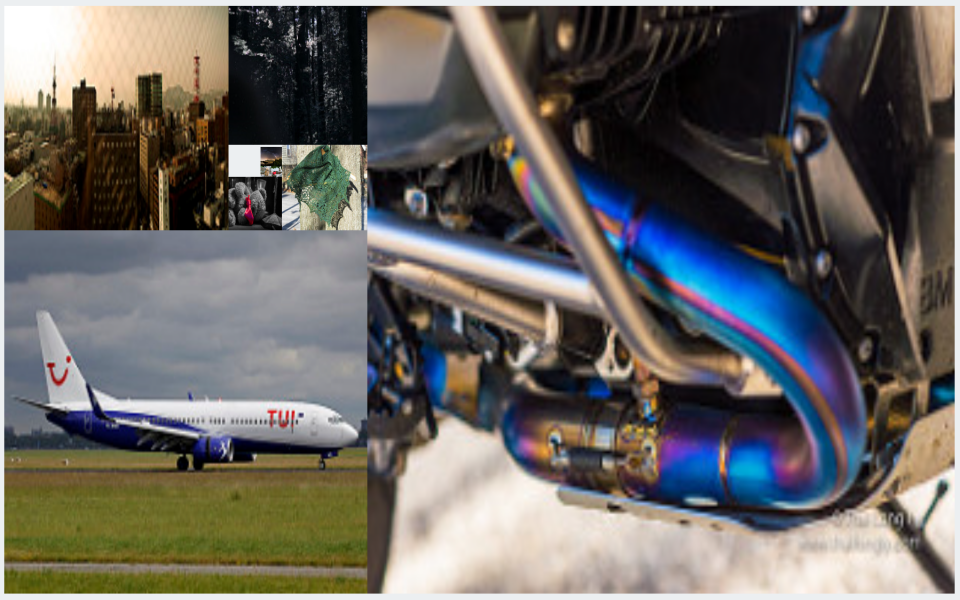
\includegraphics[width=\linewidth]{bluekittenflickr}
\caption[Image spiral `blue kitten'---Flickr]{Image spiral for query `blue kitten'---Flickr}
\label{fig:imgspiralflickr}
\end{figure}

\paragraph{Getty:}
\begin{quotation}
  \begin{description}
  \vspace{-1cm}
    \item[keyword\_ids] Return only images tagged with specific keyword(s). Specify using a comma-separated list of keyword Ids. If keyword Ids and phrase are both specified, only those images matching the query phrase which also contain the requested keyword(s) are returned.
    \item[phrase] Search images using a search phrase.
  \end{description}
  \sourceatright{\autocite{GettyAPI}}
\end{quotation}

Getty uses the \py{phrase} parameter to set the query. It only creates one pataphysicalised query term from the original query and calls for ten results based on that. This decision was based on the quota restrictions\marginpar{§~\ref{s:quota}} defined by Getty. Their limit is based on calls per second rather than calls per day or month. This means we cannot run ten calls for each user query as we did with Flickr. The query ``blue kitten'' gets turned into the word ``racy'' which then calls the \ac{API} to retrieve ten results (see figure~\ref{fig:imgspiralgetty}\marginpar{\faicon{picture-o}~\ref{fig:imgspiralgetty}}). The results mostly show racing cars from various angles although one oddball snuck in too: an office scene Getty has deemed to be `racy' (a guy in a suit checking out a lady's behind while she's leaning over a laptop).

\begin{figure}[!htbp]
\centering
  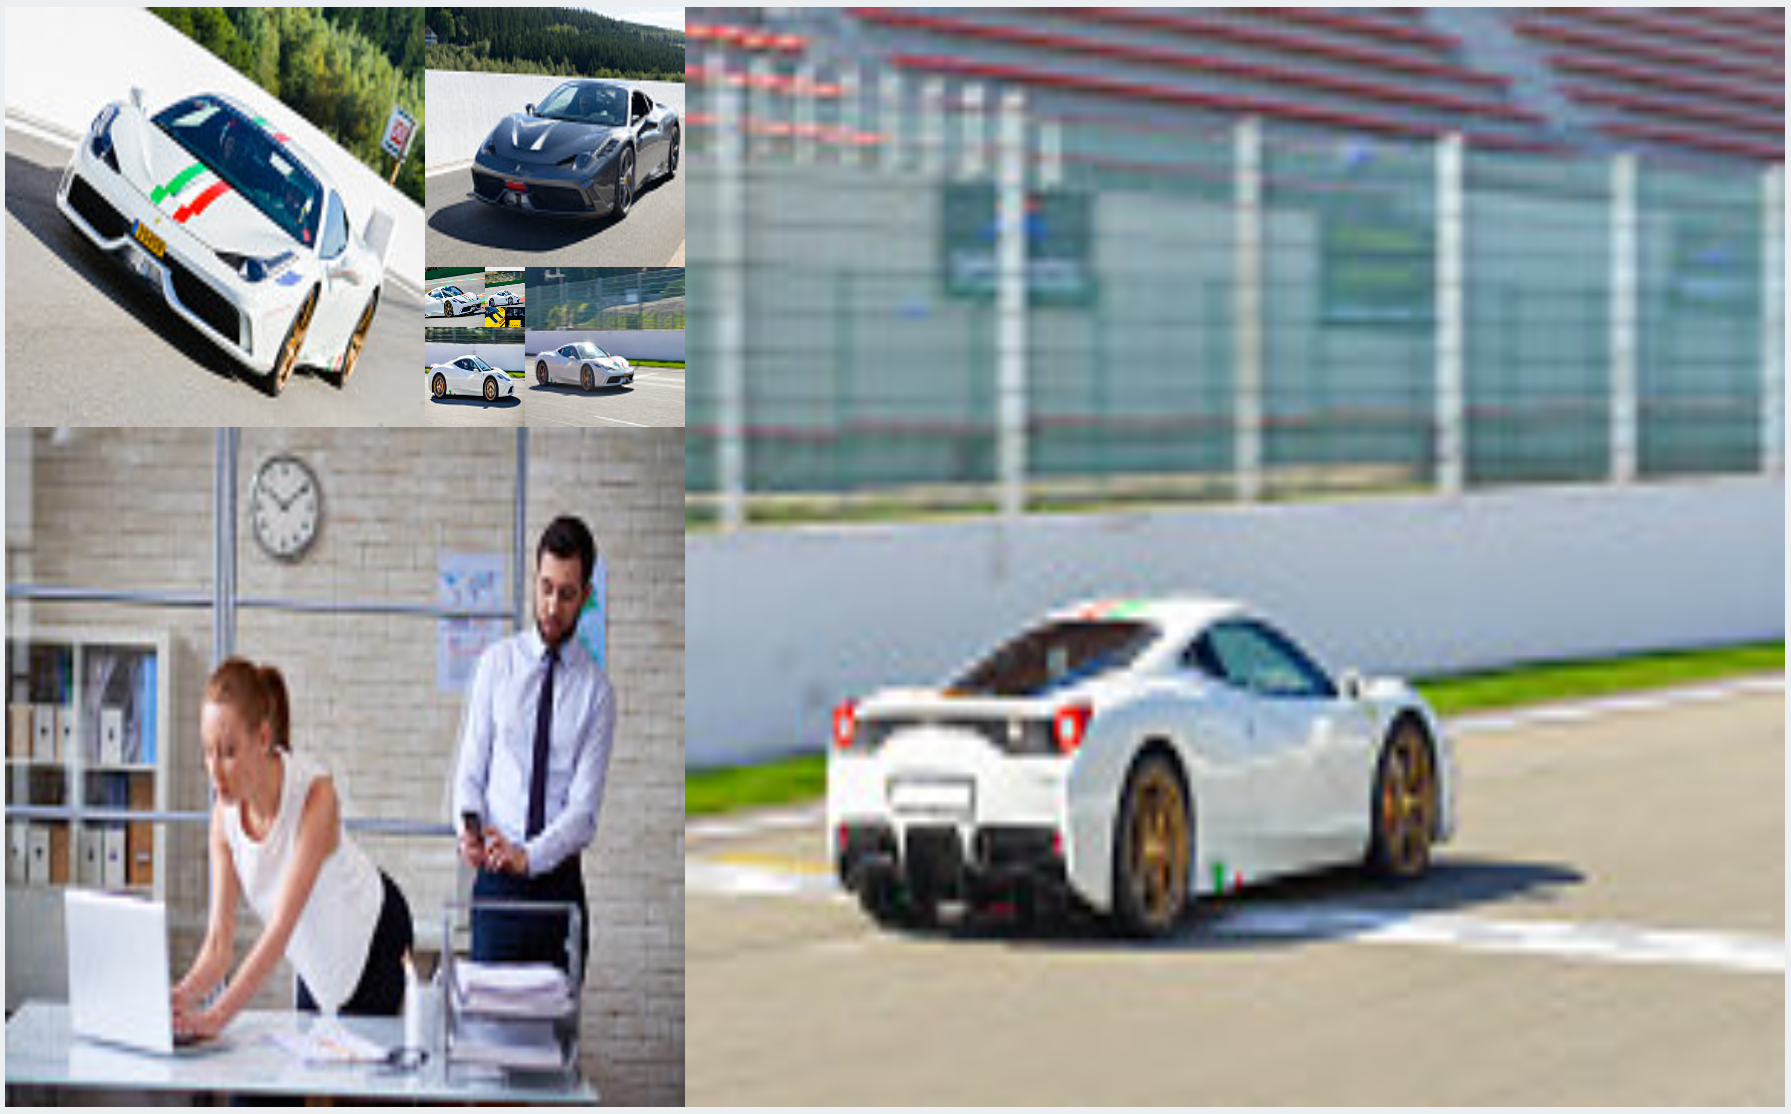
\includegraphics[width=\linewidth]{bluekittengetty}
\caption[Image spiral `blue kitten'---Getty]{Image spiral for query `blue kitten'---Getty}
\label{fig:imgspiralgetty}
\end{figure}

\paragraph{Bing:}
\begin{quotation}
  \begin{description}
  \vspace{-1cm}
    \item[query] The user's search query string. The query string cannot be empty. The query string may contain Bing Advanced Operators\footnote{For example `AND', `OR', `imagesize:', `NOT', or `phrase'}. For example, to limit images to a specific domain, use the site: operator. To help improve relevance and the results, you should always include the user's query string in an insights query (see insightsToken). This parameter is supported only by the Image API; do not specify this parameter when calling the Trending Images API.
  \end{description}
  \sourceatright{\autocite{BingAPI}\footnote{Microsoft will discontinue the current \ac{API} in December 2016. The new service will not be free unfortunately \autocite{BingNew}, so I will probably have to disable the Bing image search option.}}
\end{quotation}

The Bing function uses the \py{query} parameter to set the query in the same way as Getty.

\paragraph{YouTube:}
\begin{quotation}
  \begin{description}
  \vspace{-1cm}
    \item[q] The q parameter specifies the query term to search for. Your request can also use the Boolean NOT (-) and OR (|) operators to exclude videos or to find videos that are associated with one of several search terms. For example, to search for videos matching either ``boating'' or ``sailing'', set the q parameter value to boating|sailing. Similarly, to search for videos matching either ``boating'' or ``sailing'' but not ``fishing'', set the q parameter value to boating|sailing -fishing. Note that the pipe character must be URL-escaped when it is sent in your API request. The URL-escaped value for the pipe character is \%7C.
  \end{description}
  \sourceatright{\autocite{YouTubeAPI}}
\end{quotation}

Youtube works in a similar way too. The \py{q} parameter is set to the pataphysicalised query term and one call retrieves ten results.


\subsubsection{Quota}
\label{s:quota}

Each \ac{API} has a different quota for their subscription packages. At this stage this is not a problem but if usage of \url{pata.physics.wtf} were to increase by a lot then these limitations would cause issues. At that point there are two options: (1) live with these limits or (2) get funding to upgrade the subscriptions to these services.

\begin{description}
  \item[Flickr] \num{3600} queries per hour are free \autocite{FlickrGuideAPI}.
  \item[Getty] \num{5} calls per second, unlimited calls per day \autocite{GettyOverviewAPI}.
  \item[Bing] \num{5000} transactions per month are free. A transaction is one request that returns one page of results \autocite{BingAzureAPI}.
  \item[YouTube] \num{50000000} units per day, \num{300000} units per \num{100} seconds per user, and \num{3000000} requests per \num{100} seconds are free. A call to the video search method counts as \num{100} units \autocite{YouTubeAPI}.
  \item[Microsoft Translator] \num{2000000} characters per month are free. Note the quota relates to single characters, not words \autocite{TranslatorAPI}.
\end{description}


\section{Creativity \& Intelligence}
\label{s:theoryanalysis}

A more theoretical aspect of this analysis is concerned with what was already discussed to an extent in chapter~\ref{ch:interpretation} (specifically sections~\ref{ss:anthropomorphism}, \ref{s:programmer}, \ref{s:mimicry} and \ref{s:babying}), namely the thread connecting `artificial creativity' and \acf{AI}.

To me, the question of whether computers can be intelligent and make ethical decisions is the same as asking whether a computer can be creative. A lot of the arguments for or against \ac{AI} can be applied to computer creativity.   Answering the question of whether computers can think in my view would also answer the question of whether computers can be creative.
 
Horn groups the various strands of enquiry related to the question of `can computers think?' into 8 main arguments with several subquestions each \autocite*{Horn2009} (the full list of questions can be found in appendix~\ref{s:think}\marginpar{§~\ref{s:think}}). 

\begin{quotation}
  \begin{enumerate}
    \item Can computers think?
    \item Can the Turing test determine whether computers can think?
    \item Can physical symbol systems think?
    \item Can Chinese Rooms think?
    \item Can connectionist networks think?
    \item Can computers think in images?
    \item Do computers have to be conscious to think?
    \item Are thinking computers mathematically possible?
  \end{enumerate}
  \sourceatright{\autocite{Horn2009}}
\end{quotation}


\subsection{Free Will \& Surprise}

As early as 1842, Ada Lovelace mentioned in the annotations to her translation of Menabrea's account of Babbage's \textit{Analytical Engine} that the ``Analytical Engine has no pretensions whatever to \emph{originate} anything. It can do \emph{whatever we know how to order it} to perform'', implying that the machine cannot think by itself \autocite[][her emphasis]{Menabrea1842}.

Turing said in his article on thinking computers that ``to behave like a brain seems to involve free will, but the behaviours of a digital computer, when it has been programmed, is completely determined'' \autocite*{Turing1951}. Furthermore, in his famous article \textit{Computing Machinery and Intelligence} he mentions that a digital computer with a `random element' is ``sometimes described as having free will'' although he adds that he ``would not use this phrase'' himself \autocite*{Turing2009}. 

Introducing a random element to a computer program prevents us from fully predicting the outcome---leading to us being surprised. The ability of computers to surprise their creators seems to be an indicator of intelligence. Turing suggests that ``we should be pleased when the machine surprises us, in rather the same way as one is pleased when a pupil does something which he had not been explicitly taught to do'' \autocite*{Turing1951}. 

\begin{quotation}
  If we give the machine a programme which results in its doing something interesting which we had not anticipated I should be inclined to say that the machine \textit{had} originated something, rather than to claim that its behaviour was implicit in the programme, and therefore that the originality lies entirely with us. \sourceatright{\autocite{Turing1951}} 
\end{quotation}

% ``The more complicated the machine to be imitated the more complicated must the programme be.''\autocite{Turing1951} 


\subsection{Understanding \& Simulation}
\label{s:undersimu}

% epistemically objectivity (mountain A is higher than mountain B)
% epistemically subjectvity (mountain A is prettier than mountain B)

% ontologically objectivity (material world) - observer-independent
% ontologically subjectivity (money, itch, consciousness) - observer-relative

% Natural intelligence is observer-independent, intrinsic, conscious!
% Computer intelligence is observer-relative, not intrinsic

Strong \ac{AI}, sometimes called \ac{AGI} or true \ac{AI}, is the idea of human-level intelligence in machines. Searle speaks against the possibility of this using his famous `Chinese Room' argument amongst others. His argument breaks down into the following juxtapositions \autocite*{Searle1990,Searle2015}.

\begin{itemize}
  \item Syntax is not semantics.
  % \item Syntax is observer-relative (subjective).
  \item Semantics is not intrinsic to syntax.
  \item Simulation is not duplication.
  % \item Computation is observer-relative (subjective).
  \item Ontologically subjective topics (such as consciousness or creativity) can be studied in epistemically objective ways.
\end{itemize}

The Chinese Room thought experiment goes like this: imagine a room with two holes. On one side a question written on paper in Chinese goes in and on the other side a piece of paper comes out with the correct answer to the question, also in perfect Chinese. Inside the room sits a person with a Chinese language rulebook (written completely in English) who processed the question simply by looking up syntax, applying rules given in the instructions book and writing down the answer which to him looks like gibberish. The question then is whether or not the person inside the room `understands' Chinese.

Of course we could argue that it is not the person inside the room that understands Chinese but the room as a complete entity. It could be said the room does not `understand' Chinese, it `simulates' an understanding of it. Searle essentially argues that simulation cannot be considered strong \ac{AI}.

\begin{quotation}
  Programs are formal or syntactical. Minds have a semantics. The syntax by itself is not sufficient for the semantics. \sourceatright{\autocite{Searle2015}}
\end{quotation}

This goes back to the argument highlighted in the list above, that syntax is not semantics. The room can read and interpret the syntax and act upon rules regarding that syntax, but it cannot understand the meaning, i.e. the semantics of the Chinese words written on that paper.

\begin{quotation}
  Insofar as we can create artificial machines that carry out computations, the computation by itself is never going to be sufficient for thinking or any other cognitive process because the computation is defined purely formally or syntactically. Turing machines are not to be found in nature, they are found in our interpretations of nature. \sourceatright{\autocite{Searle2015}}
\end{quotation}

So, Searle argues a computer needs a semantical understanding of concepts in order to be considered `thinking' machines.

% \begin{quotation}
%   If computation is defined in terms of the assignment of syntax then everything would be a digital computer, because any object whatever could have syntactical ascriptions made to it. You could describe anything in terms of 0's and 1's.

%   The ascription of syntactical properties is always relative to an agent or observer who treats certain physical phenomena as syntactical.\sourceatright{\autocite{Searle1990}}
% \end{quotation}

% \begin{quotation}
%   All observer relative phenomena are created by human and animal consciousness but the human or animal consciousness that creates them is not itself observer relative.\sourceatright{\autocite{Searle2015}}
% \end{quotation}

% Human are more likely to call something AI than they would call something comp creat.
% people project human values onto machines, and human desires too. so the big bad robot uprising is a fear of what humans would do if they feel superior.

% Gödel's incompleteness theorems said that every non-trivial formal system is either incomplete or inconsistent.


\subsection{Brain \& Computers}
\label{s:braincomp}

Searle defines the three main paradigms for studies relating to computers and brains as follows \autocite*{Searle1990}.

\begin{description}[leftmargin=4cm]
  \item[Strong AI] the view that all there is to having a mind is having a program.
  \item[Weak AI] the view that brain processes (and mental processes) can be simulated computationally.
  \item[Cognitivism] the view that the brain is a digital computer.
\end{description}

Semantically, a `computer' is a person or machine that computes/calculates things---so perhaps a machine's \ac{CPU} and a human's brain are more similar than appears. If a human brain enables us to compute and we interpret computing as thinking, then surely a computer can think too?

\begin{quotation}
  Well, if computation isn’t sufficient for thinking, then what is? What is the relation between the mind and the brain, if it is not the same as the relation of the computer program to the hardware? At least the computational theory of the mind has a solution to the mind-body problem. The mind is to the brain as the computer program is to the computer hardware. If you are rejecting that solution, you owe us an alternative solution.\sourceatright{\autocite{Searle1998}}
\end{quotation}

Chatham talks about ``10 important differences between brains and computers'' \autocite*{Chatham2007} which serve as a good introduction to the topic at hand.

\begin{quotation}
  \begin{enumerate}
    \item Brains are analogue; computers are digital
    \item The brain uses content-addressable memory
    \item The brain is a massively parallel machine computers are modular and serial
    \item Processing speed is not fixed in the brain; there is no system clock
    \item Short-term memory is not like RAM
    \item No hardware/software distinction can be made with respect to the brain or mind
    \item Synapses are far more complex than electrical logic gates
    \item Unlike computers, processing and memory are performed by the same components in the brain
    \item The brain is a self-organising system
    \item Brains have bodies
    \item	The brain is much, much bigger than any [current] computer
  \end{enumerate}
\end{quotation}

To bring this into perspective Kurzweil claims the human brain is capable of $10^{16}$ operations per second \autocite*{Kurzweil2013}. Computer performance is measured in \ac{FLOPS}. The current highest ranking supercomputer\footnote{As of June 2016.}, the Chinese \textit{Sunway TaihuLight}, is capable of 93 petaflops \autocite{Fu2016,Top2016}.

\begin{table}[!htbp]
\centering
\caption{Metric prefixes}
\label{tab:metric}
\begin{tabu}{@{}llll@{}}
\toprule
kilo & k & $10^3$    & \num{1000}                \\
mega & M & $10^6$    & \num{1000000}             \\
giga & G & $10^9$    & \num{1000000000}          \\
tera & T & $10^{12}$ & \num{1000000000000}       \\
peta & P & $10^{15}$ & \num{1000000000000000}    \\
exa  & E & $10^{18}$ & \num{1000000000000000000} \\ 
\bottomrule
\end{tabu}
\end{table}

According to the \ac{HBP}, a mouse brain has roughly 100 million neurons---which would require a 1 petaflop supercomputer to simulate. Scaling that up to a human brain which has roughly 100 billion neurons would require computing power at the exascale ($10^{18}$ \ac{FLOPS}) \autocite{Walker2012}.

A precurser to the \ac{HBP}, the `Blue Brain Project' is aiming to build a supercomputer capable of $10^{18}$ \ac{FLOPS} by 2023 \autocite{Kurzweil2013}.

In a report to the \ac{EU} in 2012, the \ac{HBP} lists one of the main challenges for their research to be the computational power and energy consumption of the kind of supercomputer needed to simulate a human brain.

The human brain consumes between 16 and 30 watts, the same as an electric light bulb \autocite{Walker2012,Jabr2012}. Supercomputers have a typical energy consumption of a maximum of 20 megawatts \autocite{Walker2012}. The \textit{Sunway TaihuLight} for example uses 15 megawatts \autocite{Fu2016}. IBM's Watson on the other hand, depends on ninety servers, each of which requires around one thousand watts (so about 90 kilowatts) \autocite{Jabr2012}.

The \ac{HBP} plans to build a supercomputer at the petascale with 50 petabytes of memory, 50 petaflops and less than 4 megawatts power consumption for 2017. Their long-term goal is to reach the required exascale machine with 200 petabyte memory and 1 exaflop performance for 2021 \autocite{Walker2012}.

% average domestic home 11,072.4W is roughly 11kW \autocite{Gov2012}
% 110.1 MTOE (Million tons of oil equivalent) UK energy production 2013 = 1280463000 MWh and 190 MTOE UK energy use 2013 = 2221330000 MWh \autocite{World2016}

What this comes down to is that we are several years away from even being able to properly `simulate' a human brain, not to mention `replicate' and understand what all these neurons firing actually means in terms of `thinking'. 

\begin{quotation}
  All of our mental states, everything from feeling pains to reflecting on philosophical problems, is caused by lower level neuronal firings in the brain. Variable rates of neuron firing at synapses, as far as we know anything about it, provide the causal explanation for all of our mental life. And the mental processes that are caused by neurobiological processes are themselves realized in the structure of the brain. They are higher level features of the brain in the same sense that the solidity of this paper or the liquidity of water is a higher level feature of the system of molecules of which the table or the water is composed.

  To put this in one sentence, the solution to the traditional mind-body problem is this: Mental states are caused by neurobiological processes and are themselves realized in the system composed of the neurobiological elements.\sourceatright{\autocite{Searle1998}}
\end{quotation}

Turing once stated that ``digital computers have often been described as mechanical brains'' \autocite*{Turing1951}. Schulman analyses this analogy further \autocite*{Schulman2009}.

\begin{quotation}
  People who believe that the mind can be replicated on a computer tend to explain the mind in terms of a computer. When theorizing about the mind, especially to outsiders but also to one another, defenders of artificial intelligence (AI) often rely on computational concepts. They regularly describe the mind and brain as the `software and hardware' of thinking, the mind as a `pattern' and the brain as a `substrate', senses as `inputs' and behaviors as `outputs', neurons as `processing units' and synapses as `circuitry', to give just a few common examples. \sourceatright{\autocite{Schulman2009}}
\end{quotation}


% ``At the level of its basic operations, a computer is both extremely fast and exceedingly stupid''

% ``The power of the computer derives not from its ability to perform complex operations, but from its ability to perform many simple operations very quickly.''

Schulman lists the different layers of abstraction in computers as shown in the left column of table~\ref{tab:abstr}\marginpar{\faicon{table}~\ref{tab:abstr}} with the right column showing my attempt of defining what those layers could be in the human brain. This is a subjective approximation and serves to highlight the problems of such a comparison.

\begin{table}[!htbp]
\centering
\caption{Layers of abstraction in computers vs brains}
\label{tab:abstr}
  \begin{tabular}{@{}lcl@{}}
  \toprule
  \textbf{Computer} & \multirow{6}{*}{$\updownarrow$} & \textbf{Brain} \\ 
  \midrule
  user interface                  &  & senses and speech \& actions \\
  high level programming language &  & thinking            \\
  machine language                &  & synapses            \\
  processor microarchitecture     &  & anatomical regions  \\
  Boolean logic gates             &  & neurons             \\
  transistors                     &  & dendrites and axons \\ 
  \bottomrule
  \end{tabular}
\end{table}

\begin{quotation}
  In the black box view of programming, the internal processes that give rise to a behavior are irrelevant; only a full knowledge of the input-output behavior is necessary to completely understand a module. Because humans have `input' in the form of the senses, and `output' in the form of speech and actions, it has become an AI creed that a convincing mimicry of human input-output behavior amounts to actually achieving true human qualities in computers. \sourceatright{\autocite{Schulman2009}}
\end{quotation}

Schulman's quote above of course refers to the Turing test and its limitations (see chapter~\ref{s:mimicry}\marginpar{§~\ref{s:mimicry}}).

\begin{quotation}
  The weaknesses of the computational approach include its assumption that cognition can be reduced to mathematics and the difficulty of including noncognitive factors in creativity. \sourceatright{\autocite{Mayer1999}}
\end{quotation}

Searle also addressed this issue further, arguing that computer programs cannot possibly `think' since they are based on symbol manipulation (i.e. syntax) and don't understand what these symbols mean. He says, ``the argument rests on the simple logical truth that syntax is not the same as, nor is it by itself sufficient for, semantics'' \autocite*{Searle1990}.

\begin{quotation}
  \ldots the wisest ground on which to criticise the description of digital computers as `mechanical brains' or `electronic brains' is that, although they might be programmed to behave like brains, we do not at present know how this should be done. \sourceatright{\autocite{Turing1951}} 
\end{quotation}

Leading on to the topic creativity, it is perhaps suitable to finish with a quote by Harold Cohen on the relationship of machines and humans.

\begin{quotation}
  It's twenty years since I first realized that I could never turn AARON into a colorist by having it emulate my own expertise; in that case simply because it lacked the hardware upon which that expertise depended. Now I have AARON exercising an algorithm that couldn't be emulated by human colorists, presumably because they lack the hardware to do what AARON does. \sourceatright{\autocite{Cohen2007}}
\end{quotation}


\subsection{Creativity}

Harold Cohen created \textit{AARON}, ``perhaps the longest-lived and certainly the most creative artificial intelligence program in daily use'', in 1973 \autocite{Cohen2016}. \textit{AARON} is capable of composing and colouring drawings although later on Cohen took over the colouring part and let \textit{AARON} concentrate on composing and outlining the drawings. They exhibited in various galleries around the world and the Victoria and Albert museum in London has a sizable collection for instance \autocite{VA2016}.

Cohen argued that ``after decades of expert systems built to simulate human expertise, AARON has emerged as an expert in its own right'' and that he is ``significantly more inventive and infinitely more productive than [he] ever was [himself]'' \autocite*{Cohen2007}.

This is perhaps the opposite approach the \ac{OULIPO} has taken.

\begin{quotation}
  [The use of computers] became an instrument, not of combinatorial accumulation, but of anti-combinatorial reduction. It served not to create combinations but to eliminate them. \sourceatright{\autocite{Mathews2005}}
\end{quotation}


\subsection{State of the Art}

\ac{AI} and robotics is alluring as a research topic because it is so prevelant in science fiction and as such very present in media. Computer creativity, however, rarely plays a central role. We can regularly read headlines that tell us that yet another kind of \ac{AI}-bot has won some game against a human player. Or we see videos of some innovative ground-breaking kind of new robot which claims to be near human-like (and yet cannot walk up stairs easily or hold a decent conversation). There are many examples of advances that are hailed as the next big thing (such as in \ac{VR}) which aren't all that great in the grand scheme of things. 

Four examples I want to mention here are IBM's Watson, Microsoft's Twitter \ac{AI} chatbot Tay, Google's AlphaGo and Hanson Robotics Sophia robot.

\subsubsection{Watson} 
Watson is a question answering expert system which famously won against human Jeopardy! champions in 2011 \autocite{IBM2016}. Information lookup is an arguably fairly easy and straightforward process within \ac{IR} and as an expert system it has had noteworthy successes \autocite{Fingas2016}. Although it has similarly received subtle criticism too, such as Randall Munroe's 2015 XKCD comic on the ``Watson Medical Algorithm'' \autocite*{Munroe2015}. Similarly, Searle criticised Watson arguing that it is an ``ingenious program---not a computer that can think'' \autocite*{Searle2011}.

\subsubsection{Tay}
Tay is a Twitter chatbot. It went viral in early 2016 when it was released and then taken offline again on the same day---only to return a few days later and have the same thing happen again. The official website is only accessible as a cached version through the Internet Archive Wayback Machine \autocite{Tay2016}, although the Twitter profile is still online, but set to private \autocite{Tayandyou2016}. Hunt from the \textit{Guardian} managed to summarise the event is one sentence: ``Microsoft's attempt at engaging millennials with artificial intelligence has backfired hours into its launch, with waggish Twitter users teaching its chatbot how to be racist'' \autocite*{Hunt2016}. A week later it was briefly put online again but had to be stopped as it was repeatadly spamming its followers with the line ``You are too fast, please take a rest \ldots'' \autocite{Gibbs2016}.

\subsubsection{AlphaGo}
AlpgaGo recently won against a human professional player in the game of Go \autocite{DeepMind2016,Hassabis2016}. 

\begin{quotation}
  AlphaGo combines an advanced tree search with deep neural networks. These neural networks take a description of the Go board as an input and process it through 12 different network layers containing millions of neuron-like connections. One neural network, the `policy network', selects the next move to play. The other neural network, the `value network', predicts the winner of the game. \sourceatright{\autocite{Hassabis2016}}
\end{quotation}

While this is surely a great example of sophisticated computer programming combined with powerful hardware, I would not consider it a breakthrough in \ac{AI}. AlphaGo is a highly specialised system with only one function: to win a Go game.

\subsubsection{Sophia}
Sophia is an android made to look like a human female \autocite{Sophia2016,Hanson2016}. She\footnote{I am anthropomorphising `her' consciously here. Her website is written in first person, perhaps to make it appear like a blog written by a conscious being.} made headlines in 2016 when she announced she will ``kill all humans''. She was created using ``breakthrough robotics and artificial intelligence technologies'' and her main feature appears to be the mimicking of human facial expressions. Sophia herself says she ``can serve [humans], entertain them, and even help the elderly and teach kids'' \autocite*{Sophia2016}, although how exactly she would do that is unclear. She has two mechanical arms but no legs and there is no description of what she can do with these arms.

Life-like robots like Sophia still live in the `uncanny valley'\footnote{The philosphical zombies I mentioned in chapter~\ref{ch:interpretation} live in this uncanny valley too.}. Her voice is creepy and unhuman, her intelligence or her capabilities of understanding conversations are clearly flawed (as shown by her viral remark about supporting genocide).

\spirals

To me it seems the real breakthrough happens when (and if) the first robots appear which aren't as big as a house, can play Go, Chess \textit{and} hide-and-seek, geniunely manages to get around the uncanny valley effect, has vast knowledge in his memory for instant information lookup, can hold a normal conversation without starting a war, etc. All of the examples listed above are what I would consider expert systems. 

The \ac{AI} we know from science fiction is probably what we would consider \ac{AGI}. Perhaps this also relates to the concepts of P and H creativity mentioned in chapter~\ref{s:pandh}\marginpar{§~\ref{s:pandh}}. The systems above, like AlphaGo, may be P-intelligent rather than H-intelligent.


\section{Design}
\label{s:designanal}

It is interesting to note how different the search results are perceived when presented in a different style (e.g. list rather than poem). This could be studied using questionnaires and interviews or eye tracking tools to find out what users prefer or perceive as more creative for example (see chapter~\ref{ch:future}\marginpar{§~\ref{ch:future}}). 

Images~\ref{img:qpoemtree}, \ref{img:listsourcetree} and \ref{img:listalgotree} seen on pages~\pageref{img:qpoemtree},\pageref{img:listsourcetree} and \pageref{img:qpoemtree} respectively, show the visual difference in design for the three different display methods for text results.

The poetry\marginpar{\faicon{picture-o}~\ref{img:qpoemtree}} is compact and invites users to read all 14 (or less) lines. The two list styles\marginpar{\faicon{picture-o}~\ref{img:listsourcetree}~\&~\ref{img:listalgotree}} are much longer and involve a lot of scrolling to navigate, which might deter users from actually reading many of the results.

Personally I feel that the poetry results are automatically read with more gravity. Sorting by sources or algorithms is a game of exploration---finding the similarities within the result sets. They are different ways to view the same things and yet have a drastic influence on how the results are perceived. 

This also applies to the image and video search. Presenting results in spiral form is weird. It's hard to see where one image ends and another starts, they just kind of blur into each other. However when listed as a list they immediately become more boring.


\section{Limiting Factors}

\subsection{Biases}

\begin{quotation}
  Biases can be observed in information retrieval in situations where searchers seek or are presented with information that significantly deviates from the truth. There is little understanding of the impact of such biases in search. \sourceatright{\autocite{White2013}}
\end{quotation}

The Cambridge Dictionary defines `bias' as ``the action of supporting or opposing a particular person or thing in an unfair way, because of allowing personal opinions to influence your judgment'' or ``the fact of preferring a particular subject or thing'' \autocite*{CamDict}.

Biases can be good and bad. It is important to consider the implications of their existence though, especially when trying to measure the success of something objectively. An example of when biases can be advantageous is location signals that the search tool takes into account when producing results. An Englishmen would probably not have much use of a Chinese website and vice-versa, even if the actual content matches the original query (unless of course the user happens to understand both languages perfectly). Another example of this is location queries such as `Chinese restaurants in Cambridge', which should return web pages about restaurants based in Cambridge, UK or Massachusetts, USA, depending on the user's IP address.  This might seem logical, but in the truest sense it is a bias employed by the search engine to help provide more relevant results to individuals. Truly unbiased search results are probably impossible to come by nowadays.

There is a general move from objectivity to subjectivity in the sense that users become the subject of search results as much as the query they pose. Instead of neutrally providing results for a query alone, the results are tailored around the information known about the user (e.g.\ language, location, clickstream, social media likes, bookmarks, etc.) to make up the missing context. The user becomes the subject and context of a query, while the results become an objective list of matches for all those values rather than just the query term (s).

So in standard web search we now have the user as the subject and the results as the object. In creative search this may be reversed: the user is the object and the results become the subject.


\subsection{Constraints}

There are certain factors and constraints that influence the perception and success of search results. Some can be taken into account when building a search system but others cannot be avoided. User education is one way to deal with those issues. External constraints such as the setting in which the search takes place come to mind. Is the user operating from a handheld device or a desktop computer? Is he or she in a hurry to find answers or just leisurely browsing for them? Is the search system web-based or is the user querying a database?

\paragraph{User Expectations} It is important to note that ``search systems are not used in isolation from their surrounding context, i.e. they are used by real people who are influenced by environmental and situational constraints such as their current task'' \autocite{White2004}. User expectations should be taken into consideration during the evaluation of search results. Users who are hoping to find precise answers to a specific question might not be satisfied by exploratory search results. Someone browsing for inspiration on a broad topic on the other hand could benefit from them. Fewer expectations (an open mind) allow creativity to happen more easily. Empirical experiences form expectations, which hinder our ability to accept creative ideas when they happen. In order to be able to recognise creative ideas we need to be able to see what they all have in common and in what way they differ and not reject unusual, unexpected ones. We can link this very nicely to the idea of exploratory search. Lowering expectations or opening the mind implies extending the task domain or problem space. 

\paragraph{User Skill} The searching skills of a user matter. Specifically his or her ability to articulate an \acf{IN} and any knowledge of special search techniques (use of Boolean modifiers, quotation marks, wildcards, etc.) are two important factors that influence the results obtained greatly. This is very much based on the old idea of `garbage-in, garbage-out' \autocite{Lidwell2010}.

\paragraph{Visual Representation} The way that results are presented affects how the user perceives them. A diversity of different document types, for example text, images, sound, or video results could improve how well the results are rated \autocite{Sawle2011}. An alphabetical list is a typical model for representing text data sets for example. But a ranked list might not be the best way to represent search results. Other models could be a differently ranked or ordered list, a tree structure, a matrix, a one-to-many relationship, etc. See also section~\ref{s:designanal}\marginpar{§~\ref{s:designanal}}.

\paragraph{Structure of Results} As suggested by Sawle et al \autocite*{Sawle2011} we need to consider different ways to structure and measure search results. A single, perfectly good result might be deemed irrelevant and useless if it is surrounded by several unsuitable results. Therefore there might be certain advantages to measuring and evaluating the value or relevance of individual results over a whole set of results.

\paragraph{Direct User Relevance Feedback} Relevance feedback lets users rate individual results or sets of results either directly (through manual ratings) or indirectly (through click-stream data). This data is then congregated and used for webpage rankings or other purposes such as suggesting other query terms. It can improve results for similar queries in the future but also lets the user stir the direction his search is taking in real-time. Users can adjust their query to manipulate the results; this basically means they adjust some of their own constraints.

\begin{quotation}
  Relevance feedback---asking information seekers to make relevance judgments about returned objects and then executing a revised query based on those judgments---is a powerful way to improve retrieval. \sourceatright{\autocite{Marchionini2006}}
\end{quotation}

\paragraph{Automatic Query Expansion} As opposed to integrating and involving the user actively in the refinement of a query, in automatic query expansion the improvements are done passively, often completely without the user’s knowledge. Information gathering methods include, for example, the analysis of mouse clicks, so called like buttons (e.g. Facebook, Google+) or eye tracking, etc. How the collected data is then used varies. Simple examples of automatic query expansion are the correction of spelling errors or the hidden inclusion of synonyms when evaluating a query.

\spirals

Depending on these factors and constraints, search results can be viewed as useful or useless. In a way the usefulness or correctness of an idea or result cannot always be judged fairly – there are always conditions that will affect how the outcome is interpreted. In the scenario of a creative search tool, results could be very useful, while they might be completely useless in another.

We would need to investigate each individual search result in terms of its value and creativity. This could be done by user ratings or satisfaction questionnaires. Rather than measuring the success of individual results we could look at evaluating them as one set instead.

The search results produced by \url{pata.physics.wtf} can be quite surprising sometimes and it is not always clear how they connect to the initial query (especially if the inner workings of the algorithms are unknown), even if we identify through which function a result has been obtained. The names of these algorithms might not be helpful to users though if they are unfamiliar with the concept of pataphysics and might therefore appear rather nonsensical. Whilst there is a clear logic to each search result, they might appear anomalous to the user's expectations if he or she received these results without knowing the philosophy of the search tool. The results could possibly appear random then, and might therefore appear useless to the user.


\section{Meta Analysis}

The code for \url{pata.physics.wtf} and this thesis written in \LaTeX \ and are both kept under git version control \autocite{Git2016}.

\begin{quotation}
  The name `git' was given by Linus Torvalds when he wrote the very first version. He described the tool as `the stupid content tracker' and the name as (depending on your mood):
  \begin{itemize}
    \item random three-letter combination that is pronounceable, and not actually used by any common UNIX command. The fact that it is a mispronunciation of `get' may or may not be relevant.
    \item stupid. contemptible and despicable. simple. Take your pick from the dictionary of slang.
    \item `global information tracker': you're in a good mood, and it actually works for you. Angels sing, and a light suddenly fills the room.
    \item `goddamn idiotic truckload of sh*t': when it breaks 
  \end{itemize} \sourceatright{\autocite{Git2016}}
\end{quotation}

\begin{figure}[!htbp] % (here, top, bottom, page)
  \centering
  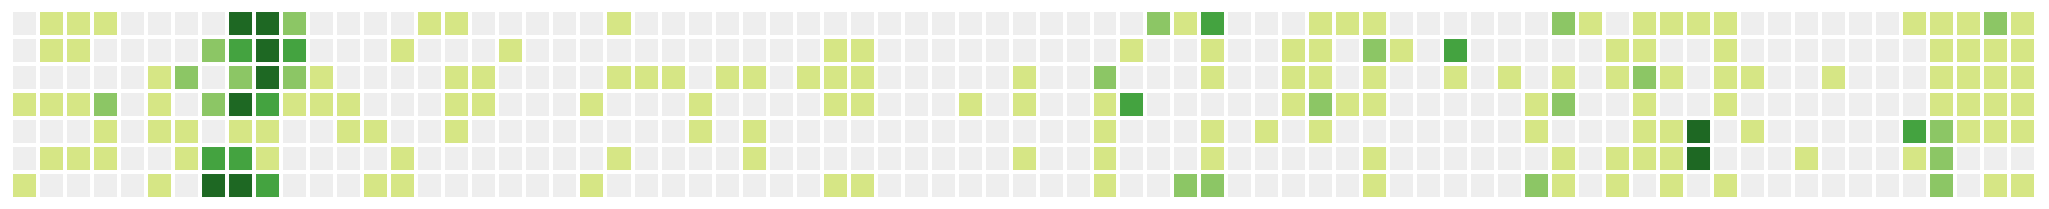
\includegraphics[width=\linewidth]{images/github0}
\caption[GitHub contributions]{GitHub contributions for code and thesis}
\label{img:github}
\end{figure}

Both repositories (folders which contain the files to be monitered) are stored remotely on GitHub \autocite*{GitHub2016} and synced with the local machine. Image~\ref{img:github}\marginpar{\faicon{picture-o}~\ref{img:github}} shows the contribution history from the last 17 months for both of the \url{pata.physics.wtf} code and this thesis. A darker green indicates several commits (i.e. saves) while gray indicates no commits. Each square represents a day, each colum a week (Sunday--Saturday).

The full git commit histories for both repositories are shown in appendix~\ref{app:git}\marginpar{§~\ref{app:git}}. 


\stopcontents[chapters]
